%Documento principal do latex para uso no TCC da Univás.

\documentclass[a4paper, 12pt, chapter=TITLE, oneside, english, brazil]{abntex2}

\usepackage{styles/CodeStyle}      %Formatação de códigos e listagens
\usepackage{styles/EventFlowStyle} %Estilo para o quadro de fluxo de eventos
\usepackage{styles/NuapaStyle}     %Estilo exigido pela Univás
\usepackage[table,xcdraw]{xcolor}  %Pacote para gerar as tabelas
\usepackage{array,multirow,graphicx} %Pacote para escrever o nome dos meses da tabela em vertical
\definecolor{lightgray}{gray}{0.9} %Pacote para montar a tabela zebrada do orçamento
\usepackage{ragged2e} %Usado para justificar as referências basta colocar no arquivo Principal.bbl o \justify antes das referências. Exemplo abaixo
%\bibitem[W3C 2015]{w3c_css_definition}
%\abntrefinfo{W3C}{W3C}{2015b}
%\justify{W3C. \textbf{What is CSS?} 2015. \url{http://www.w3.org/Style/CSS/}.
%	Acesso em: 24 de julho de 2015.}

\usepackage{pdflscape}
%Início do documento
\begin{document}

\pretextual %Início dos Elementos Pré-Textuais c


\makeatletter
\renewcommand{\imprimircapa}{%
\begin{capa}%
\begin{center}%
  {\ABNTEXchapterfont\large\MakeUppercase\imprimirautor}\\
  \vspace*{\fill}%
  \vspace*{\fill}%
  \vspace*{\fill}%
  {\ABNTEXchapterfont\bfseries\Large\MakeUppercase\imprimirtitulo}\\
  \vspace*{\fill}%
  {\color{white}%
\abntex@ifnotempty{\imprimirpreambulo}{%
  \hspace{.45\textwidth}
  \begin{minipage}{.5\textwidth}
    \SingleSpacing
    \imprimirpreambulo
  \vspace{.1\textwidth}\\%
  {\imprimirorientadorRotulo:~\imprimirorientador}
  \abntex@ifnotempty{\imprimircoorientador}{%
    \hspace{.45\textwidth}
    {\large\imprimircoorientadorRotulo~\imprimircoorientador}%
  }%
  \end{minipage}%
}%
\color{black}}%
  \vspace*{\fill}\\%
  {\ABNTEXchapterfont\large\bfseries\MakeUppercase\imprimirinstituicao}\\
  {\large\bfseries\MakeUppercase\imprimirlocal}\\
  {\large\bfseries\MakeUppercase\imprimirdata}
\end{center}
\end{capa}
}
\makeatother

\imprimircapa

% folha de rosto 
%\folhaderostoname{Folha de rosto}
%http://code.google.com/p/abntex2/wiki/ComoCustomizar

\makeatletter
\renewcommand{\folhaderostocontent}{
\begin{center}%
  {\ABNTEXchapterfont\large\MakeUppercase\imprimirautor}\\
  \vspace*{\fill}%
  \vspace*{\fill}%
  \vspace*{\fill}%
  {\ABNTEXchapterfont\bfseries\Large\MakeUppercase\imprimirtitulo}\\
  \vspace*{\fill}%
\abntex@ifnotempty{\imprimirpreambulo}{%
  \hspace{.45\textwidth}
  \begin{minipage}{.5\textwidth}
    \SingleSpacing
    \imprimirpreambulo
  \vspace{.1\textwidth}\\%
  {\imprimirorientadorRotulo:~\imprimirorientador}
  \abntex@ifnotempty{\imprimircoorientador}{%
    \hspace{.45\textwidth}
    {\large\imprimircoorientadorRotulo~:\imprimircoorientador}%
  }%
  \end{minipage}%
}%
  \vspace*{\fill}\\%
  {\ABNTEXchapterfont\large\bfseries\MakeUppercase\imprimirinstituicao}\\
  {\large\bfseries\MakeUppercase\imprimirlocal}\\
  {\large\bfseries\MakeUppercase\imprimirdata}
\end{center}
}%end of folhaderostocontent
\makeatother

\imprimirfolhaderosto*{}
\begin{fichacatalografica}
\begin{normalsize}
  \vspace*{\fill}
  % Posição vertical
%  \hrule
  % Linha horizontal
  \begin{center}
  \fbox{
    % Minipage Centralizado
    \begin{minipage}[c]{12.5cm} % Largura
      \vspace{0.7cm}%
      \hspace{0.8cm} \imprimirAutorCitacao ~\\%
      
      \hspace{0.8cm} \imprimirtitulo ~/ \imprimirAutorUm , \imprimirAutorDois ~-- \imprimirlocal: Univás, \imprimirdata. %
      
      %\hspace{0.8cm} \pageref{LastPage} f. : il.~\\%
      \hspace{0.8cm} 141 f. : il.~\\%
      
      \hspace{0.8cm} \imprimirtipotrabalho~--~\imprimirinstituicao , Univás, \imprimircurso. % 
      
      \hspace{0.8cm} \imprimirorientadorRotulo: ~\imprimirorientador ~\\%

      \hspace{0.8cm} 1. \imprimirPalavraChaveUm. 2. \imprimirPalavraChaveDois. 3. \imprimirPalavraChaveTres. ~ \\%
    \end{minipage}
    }
  \end{center}
\end{normalsize}
\end{fichacatalografica}
\newpage 
\setlength{\ABNTEXsignwidth}{10cm}

\begin{folhadeaprovacao}
  \begin{center}
    {\ABNTEXchapterfont\large\MakeUppercase\imprimirautor}
    \vspace*{\fill}
    \vspace*{\fill}
    \vspace*{\fill}
    \par
    {\ABNTEXchapterfont\bfseries\Large\MakeUppercase\imprimirtitulo}
    \vspace*{\fill}
  \end{center}
  Trabalho de conclusão de curso defendido e aprovado em \imprimirDataDaAprovacao ~pela banca examinadora constituída pelos professores:

  ~\newline
  \begin{flushleft}
  \assinatura*{\imprimirorientador \\ \imprimirorientadorRotulo }
  \assinatura*{\imprimirAvaliadorUm \\ \imprimirAvaliadorLabelUm }
  \assinatura*{\imprimirAvaliadorDois \\ \imprimirAvaliadorLabelDois}
  \end{flushleft}
  \vspace*{\fill}
  \vspace*{\fill}
\end{folhadeaprovacao}

\begin{dedicatoria}
\vspace*{\fill}
\vspace*{\fill}
\vspace*{\fill}
\vspace*{\fill}
\vspace*{\fill}
\vspace*{\fill}
De \imprimirAutorUm.
\newline
%início da dedicatória do autor um
Dedico este trabalho a Deus, por guiar os meus passos e me manter firme no caminho, mesmo em meio as dificuldades. A minha mãe Regina Faria, por ser uma mulher de fibra, guerreira e tão merecedora esta conquista. Obrigada por estar comigo em todos os momentos e por ter acreditado em mim, nós conseguimos. A minha irmã Juliana Faria, por me apoiar e ser a melhor irmã que alguém poderia ter, amo você. Ao meu padrasto José Vitor, por ser um homem íntegro e cheio de bons conselhos. Ao meu tio amado, Carlos Campos, por me incentivar a ir em frente e não desistir dos meus sonhos, o seu apoio foi fundamental para esta realização. Ao meu companheiro Rubens Vilela, por toda dedicação e amor, você fez toda a diferença nesta caminhada. Agradeço por cada conselho, por ser o meu refugio em momentos difíceis, por todo o apoio. Obrigada por toda essa cumplicidade, você é especial. À todos os meus familiares. Aos meus amigos, por serem os melhores do mundo. A todos os que de alguma forma, direta ou indiretamente, contribuíram para a concretização deste sonho. Deus os abençoe.

\vspace*{\fill}
De \imprimirAutorDois.
\newline
%início da dedicatória do autor dois
Dedico este trabalho primeiramente, a Deus, pela força e coragem durante toda esta longa caminhada. A minha mãe Cleide de Souza Justiniano, que apesar de todos os contra tempos sempre esteve ao meu lado em todos os momentos, sejam eles difíceis ou não, desde minha infância. A meu pai Venicius Justiniano, exemplo de pessoa, que me mostrou o caminho das pedras, fazendo com o que eu me tornasse o homem que sou hoje. A meus irmãos pelo apoio e companheirismo. A meus avós, que sempre me incentivaram a estudar em busca de um futuro melhor, principalmente a minha avó Maria Aparecida do Prado (\textit{in memoriam}) que me viu iniciar esta caminhada, porém, não pode me ver finalizá-la. À minha noiva Josy, pessoa com quem amo partilhar todos os momentos da vida. Com você tenho me sentindo mais vivo e feliz. Obrigado pelo carinho, paciência, compreensão, parceria e por sua capacidade de me trazer alegria e paz na correria de cada semestre, sempre acreditando, apoiando e me incentivando desde o princípio. À meus amigos por estarem sempre ao meu lado. Aos meus demais familiares por confiarem em mim. À aqueles que direto ou indiretamente contribuíram para que eu alcançasse mais essa vitória em minha vida. Obrigado a todos!
\end{dedicatoria}

\begin{agradecimentos}

Agradecemos,
\newline

%Início agradecimentos em conjunto
\par A Deus, por tudo. Que todas as coisas sejam para a Tua honra e glória.

\par Ao orientador Márcio Emílio, por todo apoio, incentivo e amizade, demostrados não somente neste trabalho mas em todo o período da faculdade.

\par À professora Joelma Faria, que por sua leitura minuciosa nos ajudou para que este trabalho alcançasse sua melhor versão.

\par Aos professores Roberto Rocha e André Martins pelas dicas que contribuíram para a melhorar a qualidade deste trabalho.

\par Ao professor e coordenador José Luiz, por todo apoio e suporte.

\par A todos os professores e colegas de classe, pela amizade, conselhos e todo o conhecimento compartilhado.

\vspace*{\fill}
De \imprimirAutorUm
\newline
%início do agradecimento do autor um

\par Ao meu amigo e parceiro Edilson Justiniano por toda dedicação, compreensão e apoio. Por ser tão incrível e prestativo, se tonando fundamental para a concretização deste trabalho. Muitas vezes foi meu professor, mas acima de tudo, foi e será sempre um grande amigo do qual eu me orgulho muito.

\par Aos meus amigos Sandro Augusto e Jonathan Santos, por todo incentivo e apoio contínuo. Pela amizade que se enraizou no decorrer destes anos de luta.

\par Aos meus familiares, por todo carinho e amor. Em especial a minha mãe, por ser a minha base, me incentivando sempre a buscar e fazer o melhor. 

\par Ao meu querido Rubens Vilela, por estar sempre do meu lado, a cada passo, se fazendo essencial e me sustentando em todas as etapas desta caminhada.

\par A todos os que passaram pelo meu caminho e contribuiriam de alguma forma para que eu chegasse até aqui. De coração, obrigada!


\vspace*{\fill}
De \imprimirAutorDois
\newline
%início do agradecimento do autor dois
\par À minha parceira deste trabalho Andressa Faria Giordano pela atenção, dedicação e competência, sempre disposta a ajudar no que fosse necessário.

\par Aos amigos Sandro Oliveira e Jonathan Santos, pela amizade e apoio contínuo ao longo desses anos.

\par A minha família, de forma especial, meus pais, por contribuírem com essa realização, sempre acreditando e me incentivando a estudar em busca de um futuro melhor.

\par A minha querida Josy Chaves, obrigado por seu apoio incondicional, sempre me incentivando a fazer o meu melhor. Se tornando essencial nessa conquista.

\par Ao amigo, ex-professor e ex-patrão Túlio Faria que nos ajudou a definir algumas das tecnologias utilizadas por este trabalho.

\par Ao amigo Miller Faria por ajudar no processo de desenvolvimento deste trabalho.

\end{agradecimentos}





\begin{epigrafe}
\vspace*{\fill}
\begin{flushright}
\textit{"Cada sonho que você deixa para trás é um pedaço do seu futuro que deixa de existir."
	 (Steve Jobs)}
\end{flushright}
\end{epigrafe}

%Lista de Figuras
\pdfbookmark[0]{\listfigurename}{lof}
\listoffigures*
\cleardoublepage

%Comentar a Lista de Quadros porque até o dia 27-04-2015 não temos nenhum quadro no projeto escrito
% Lista de Quadros
\pdfbookmark[0]{\listofquadrosname}{loq}
\listofquadros*
\cleardoublepage

%Comentar a Lista de Tabelas porque até o dia 27-04-2015 não temos nenhuma tabela no projeto escrito
%Lista de Tabelas
%\pdfbookmark[0]{\listtablename}{lot}
%\listoftables*
%\cleardoublepage

%Comentar a Lista de Códigos porque até o dia 27-04-2015 não temos nenhumm código no projeto
%Lista de Códigos
\counterwithout{lstlisting}{chapter}
\pdfbookmark[0]{\lstlistingname}{lol}
%http://tex.stackexchange.com/questions/50031/how-to-remove-contents-line-from-table-of-contents
\begin{KeepFromToc}
\lstlistoflistings
\end{KeepFromToc}
\cleardoublepage

%Lista de siglas
%ver http://marc.info/?l=tex-br&m=110566665520790 para colocar em ordem alfabética.

\begin{SingleSpace}

\begin{siglas}
\item[ACID]  Atomicidade, Consistência, Isolamento e Durabilidade
\item[ACM]   \textit{Association for Computing Machinery}
\item[API]   \textit{Application Programming Interface}
\item[CSS]	 \textit{Cascading Style Sheet}
\item[HTML]	 \textit{Hypertext Markup Language}
\item[HTTP]  \textit{Hypertext Transfer Protocol}
\item[IDE]	 \textit{Integrated Development Environment}
\item[JSF]   \textit{JavaServer Faces}
\item[JSON]	 \textit{Javascript Object Notation}
\item[JSP]   \textit{JavaServer Pages}
\item[JVM]   \textit{Java Virtual Machine}
\item[MVC]   \textit{Model -- View -- Controller}
\item[MySQL] Banco de dados relacional
\item[NoSQL] \textit{Not Only SQL}
\item[REST]  \textit{Representational State Transfer}
\item[SOAP]	 \textit{Simple Object Access Protocol}
\item[SQL]   \textit{Structured Query Language}
\item[UML]   \textit{Unified Modeling Language}
\item[URI]   \textit{Uniform Resource Identifier}
\item[W3C]   \textit{World Wide Web Consortium}
\item[WSDL]  \textit{Web Service Description Language}
\item[XML]   \textit{Extensible Markup Language}

\end{siglas}

\end{SingleSpace}
				
% --- resumo em português ---

\begin{OnehalfSpacing} 

\noindent \imprimirAutorCitacaoMaiuscula. {\bfseries\imprimirtitulo}. {\imprimirdata}.  Monografia -- Curso de {\MakeUppercase\imprimircurso}, {\imprimirinstituicao}, {\imprimirlocal}, {\imprimirdata}.

\vspace{\onelineskip}
\vspace{\onelineskip}
\vspace{\onelineskip}
\vspace{\onelineskip}

\begin{resumo}
~\\
%início do texto do resumo
\noindent Esta pesquisa apresenta o estudo do banco de dados orientado a grafos aplicado à busca por mão de obra temporária, utilizando o mesmo modelo de negócio presente nas redes sociais. Esta pesquisa é do tipo aplicada, pois visa propor uma solução para um problema social, que acontece dentro de uma região específica, mas que pode ser útil a toda população. Para obter os resultados esperados, foi utilizado o banco de dados Neo4j, juntamente com a API \textit{Cypher}, usada para a navegação e inserção de dados no banco. Foi desenvolvido um sistema na plataforma \textit{web}, com o auxílio das tecnologias HTML, CSS Javascript e o \textit{framework} Angular JS, atuando do lado cliente da aplicação e as tecnologias Java, \textit{Web service} REST, juntamente com o Neo4j, atuando do lado servidor. Foram desenvolvidas funcionalidades que beneficiam tanto o prestador de serviço quanto o contratante, auxiliando-os na tomada de decisão. Como exemplo, pode-se citar a busca por determinado tipo de serviço, avaliação de desempenho de profissionais, criação de redes de parcerias, além de gráficos comparativos, que mostram ao usuário informações sobre as últimas avaliações. Essas funcionalidades tornaram esta pesquisa de grande relevância social, técnica e teórica por contribuir com a exploração de novos recursos, relacionados aos bancos de dados NoSQL. Com isso, conclui-se que os objetivos propostos por este trabalho foram atendidos.


%fim do texto do resumo
\vspace{\onelineskip}
\vspace*{\fill}
\noindent \textbf{Palavras-chave}: \imprimirPalavraChaveUm. \imprimirPalavraChaveDois. \imprimirPalavraChaveTres.
\vspace{\onelineskip}
\end{resumo}

\end{OnehalfSpacing}

% --- resumo em inglês ---

\begin{OnehalfSpacing} 

\noindent \imprimirAutorCitacaoMaiuscula. {\bfseries\imprimirtitulo}. {\imprimirdata}.  Monografia -- Curso de {\MakeUppercase\imprimircurso}, {\imprimirinstituicao}, {\imprimirlocal}, {\imprimirdata}.

\vspace{\onelineskip}
\vspace{\onelineskip}
\vspace{\onelineskip}
\vspace{\onelineskip}

\begin{resumo}[Abstract]%
\begin{otherlanguage*}{english}%
\textit{
%início do texto do abstract
\noindent This academic research presents the study about the graph database applied to search for temporary workmanship using the same business model adopted by social networks. The kind of this research is applied, since it aims to propose a solution for a real social problem that happens inside a specific region but can be helpful to entire population. It was used the graph database Neo4j, together with the API Cypher to navigate and insert data on database, in order to get the results. A web based software was developed with aid of technologies HTML, CSS, Javascript and the framework Angular JS, working in client side of application and the technologies Java, Web service REST together with Neo4j, working in server side. The functionalities to benefit the service providers as well the contractors have been developed to help them in decision-making. An example, it is possible to quote the search for a particular type of service, performance analysis of professionals, creation of partners network, beyond of comparative graphs which display to user, information about the last evaluations. These functionalities have made this research of high relevance social, technique and theoretical to contribute to exploring of news resources related to NoSQL databases. With this, it concludes that the objectives proposed by this work were met.
%fim do texto do abstract
}

\vspace{\onelineskip}
\vspace*{\fill}
\noindent \textbf{Key words}: \imprimirKeyWordOne. \imprimirKeyWordTwo. \imprimirKeyWordThree.
\end{otherlanguage*}
\vspace{\onelineskip}
\end{resumo}

\end{OnehalfSpacing}

%Sumário
%ver esse link para configuração de fonte: http://tex.stackexchange.com/questions/83377/how-to-change-chapter-font-style-in-the-middle-of-the-table-of-the-contents
\renewcommand*\contentsname{\centerline{SUMÁRIO}}
\pdfbookmark[0]{\contentsname}{toc}
\begin{SingleSpace} 
\tableofcontents*
\end{SingleSpace}
\cleardoublepage


\textual %Início dos Elementos Textuais

%\chapter*{Introdução}
\begin{flushleft}
	\vspace{1.2em}
	\textbf{\large INTRODUÇÃO}
	\vspace{2.9em}
\end{flushleft}
\thispagestyle{empty}

\addcontentsline{toc}{chapter}{INTRODUÇÃO}
\stepcounter{chapter} %incrementa o número do capítulo

\par Com a constante evolução tecnológica é possível notar que, a cada dia, mais pessoas estão se inserindo no mundo globalizado. Pertencer a este meio tem mudado completamente a maneira de se realizar tarefas, uma vez que a revolução tecnológica busca facilitar o que até então era trabalhoso. Atualmente, nos deparamos com situações nas quais as pessoas desempenham mais de um papel, dividindo o seu tempo entre tarefas profissionais, pessoais e aquelas que chamamos de rotineiras as quais muitas vezes, não são realizadas por elas e sim por terceiros.

\par Um profissional terceirizado é capaz de cuidar de todas as tarefas extras que não cabem na rotina, no entanto, encontrá-los tem se tornado cada vez mais difícil, uma vez que confiar a sua residência ou ainda, a sua intimidade a uma pessoa não conhecida gera muita insegurança. Ainda, vale ressaltar que este tipo de trabalho está cada vez mais escasso e raro no cenário atual.

\par Com o advento da internet, e mais tarde sua popularização, uma série de aplicações para diferentes fins vem sendo desenvolvidas. Estes aplicativos tem como finalidade apresentar soluções para os mais diversos tipos de problemas. É possível notar que as redes sociais geram um grande impacto no modelo de vida que as pessoas seguem, isto se deve ao fato de que tudo e todos estão conectados, direta ou indiretamente, e que as informações são trocadas a uma velocidade surpreendente, sendo necessário obtê-las de forma clara e rápida \cite{barbosa_why_people_use_social_network}.

\par% Com intuito de obter acesso à informação de maneira instantânea, a migração dos antigos computadores pessoais (\textit{desktops}) para dispositivos cada vez mais portáteis tornou-se comum. Podemos citar, como exemplo, a criação dos \textit{tablets} que proporcionaram uma grande revolução tecnológica, pois, a partir desta invenção as pessoas passaram a ter liberdade de acesso, uma vez que as informações se encontram na palma de suas mãos. Seguindo esta tendência de mobilidade, os \textit{smartphones} foram desenvolvidos.

\par %O sucesso obtido por estes dispositivos móveis, somado a evolução das redes de dados 3G e 4G, permitiu a conexão entre as pessoas de qualquer lugar e a qualquer momento bastando alguns toques, tornando assim ainda mais fácil localizá-las e comunicar-se com elas.

\par %A pesquisa realizada pelo Instituto Nielsen reafirma o contexto anteriormente mencionado. Ela comprova que o tempo gasto pelos usuários em seus \textit{smartphones} é maior do que em seus computadores pessoais, sendo que boa parte deste tempo é utilizado para acesso às redes sociais. Isto ocorre pois os dispositivos móveis atuais são capazes de substituir os computadores pessoais em uma série de atividades, tornando-os um computador de mão disponível a qualquer instante. A pesquisa, ainda demonstra o sucesso das redes sociais que, segundo a mesma, se deve a disseminação dos dispositivos móveis e ao modelo de vida que grande parte das pessoas segue atualmente.

\par Com a ampliação desta comunicação, somada à evolução das tecnologias, houve a necessidade de se realizar algumas melhorias voltadas aos bancos de dados, a fim de otimizar as tarefas realizadas por ele, levando assim, a criação de uma nova geração de bancos de dados, denominada NoSQL\footnotemark[1].

\footnotetext[1]{NOSQL: \textit{Not Only SQL} - Bancos de dados que utilizam não somente os recursos de Structure Query Language - SQL, a fim de obter melhor \textit{performance}.}

\par Dentre esta nova geração, o banco de dados orientado a grafos vem se destacando por apresentar grande potencial para manipulação de dados em diferentes áreas como: relacionamento interpessoal, biológicas, rotas geográficas, entre outras.

\par \citeonline{tcc_univas_penha_carvalho_recomendacao_filmes} utilizaram esta tecnologia para desenvolver uma aplicação, cujo principal objetivo é recomendar filmes aos seus usuários de acordo com seus gostos pessoais, utilizando o conceito de \textit{traversals} (travessias), disponibilizada pelo banco Neo4j, possibilitando a navegação pelo grafo.

\par \citeonline{tcc_univas_silva_pires_comparacao_banco_dados} realizaram uma comparação entre banco de dados orientado a grafos e os relacionais aplicados à redes sociais, a fim de apresentar as vantagens que estes possuem sob os bancos de dados relacionais. Para realizar tal comparação foi utilizada algumas consultas que possuem o mesmo fim para ambos e um simples software desenvolvido utilizando a linguagem Java para calcular o tempo gasto no processamento dessas consultas.

\par \citeonline{junid_tahir_majid_idros_potential_graph_thory_for_dna_sequence_alignment} utilizaram a teoria dos grafos para tentar otimizar o processo de alinhamento da sequência de DNA a fim de determinar a região comum entre duas ou mais sequências deste. Para determinar esta região, foi necessário além da teoria dos grafos, modificar alguns algoritmos assim como algumas fórmulas matemáticas, para se obter o resultado proposto.

\par A fim de justificar a escolha do tema, foi realizada uma pesquisa informal com o auxílio de um formulário, disponibilizado na internet, na região de Pouso Alegre. Por meio dessa pesquisa constatou-se que não há um sistema que possua como principal objetivo localizar determinados tipos de mão de obra nos quais não existam vínculos empregatícios. Esse formulário está disponível no Apêndice VI deste trabalho.

\par Este projeto propõe atuar sobre esta limitação, desenvolvendo um software cujo principal objetivo é localizar e apresentar aos usuários, profissionais temporários que possuam credibilidade e boas referências.

\par A fim de tornar possível a realização do mesmo serão utilizadas tecnologias gratuitas e de boa aceitação pelo mercado. Desta forma, será possível reduzir o custo de desenvolvimento, possibilitando a sua distribuição aos usuários. Com esta distribuição, seus benefícios alcançarão uma quantidade maior de pessoas, aumentando consideravelmente a facilidade na busca por este tipo de profissional.

\par Como o objetivo geral deste trabalho é buscar a solução de um problema relacionado à busca por mão de obra temporária, desenvolvendo uma aplicação \textit{web} utilizando uma base de dados orientada a grafos, capaz de realizar buscas por profissionais que desempenhem trabalho temporário sem vínculo empregatício formalizado. Esta aplicação seguirá como base o modelo de negócio das redes sociais, a fim de gerar a familiarização desta ferramenta, uma vez que este tipo de serviço já está intrínseco na atualidade.

\par Os objetivos específicos deste trabalho são:

\begin{itemize}
	\item Demostrar o uso do banco de dados Neo4j, por meio da \textit{Application Program Interface} API Cypher;
	\item Representar o problema utilizando grafos;
	\item Projetar e implementar uma aplicação \textit{web} para cadastro e busca de mão de obra.
\end{itemize}

\par Este projeto também visa a proporcionar uma base de conhecimentos e explanação de tecnologias atuais e valorizadas, sendo que algumas não fazem parte do escopo do curso. Agregando todos estes benefícios à possibilidade de melhoria contínua e acréscimos de novas funcionalidades, este projeto servirá como apoio para novos trabalhos acadêmicos.

\par Este trabalho é composto por quatro capítulos, e uma breve descrição de cada um deles é apresentada a seguir. O primeiro capítulo, denominado Quadro Teórico, discute todas as teorias utilizadas durante o seu desenvolvimento. No segundo capítulo, Quadro Metodológico, são demonstrados detalhes a respeito da pesquisa, como ela foi realizada, as ferramentas utilizadas, além dos procedimentos realizados até a sua finalização. No terceiro capítulo, Discussão dos resultados, são apresentados os mais relevantes resultados obtidos após a conclusão do trabalho. No quarto capítulo, denominado Conclusão, são descritas as considerações finais e impressões desta pesquisa.
%\chapter{OBJETIVOS}

\par Para que se possa levar esta proposta de pesquisa a cabo são colocados os seguintes objetivos:

\section{Objetivo geral}

\par Desenvolver uma aplicação \textit{web} utilizando uma base de dados orientada a grafos, capaz de realizar buscas por profissionais que desempenham trabalhos temporários sem vínculo empregatício.

\section{Objetivos específicos}

\begin{itemize}
	\item Demostrar o uso do banco de dados Neo4j, por meio do da \textit{Application Program Interface} API Cypher;
	\item Representar o problema utilizando grafos;
	\item Projetar e implementar uma aplicação \textit{web} para cadastro e busca de mão de obra.
\end{itemize}

\footnotetext[2]{API: \textit{Application Program Interface} -  Conjunto de funções, métodos, ferramentas e protocolos utilizados para o desenvolvimento de um \textit{software}.} %Added by Edilson Justiniano on 18-03-2015 for "Pré-projeto"
%\chapter{JUSTIFICATIVA}

\par Por meio de uma pesquisa informal, realizada com o auxílio de formulários disponibilizados na internet, na região de Pouso Alegre, foi constatado que não há um sistema que possua como principal objetivo localizar determinados tipos de mão de obra nos quais não existam vínculos empregatícios.

\par Este projeto propõem atuar sobre esta limitação, desenvolvendo um software cujo principal objetivo é localizar e apresentar aos usuários, profissionais temporários que possuam credibilidade e boas referências.
	
\par A fim de tornar possível a realização do mesmo serão utilizadas tecnologias gratuitas e de boa aceitação pelo mercado. Desta forma, será possível reduzir o custo de desenvolvimento, possibilitando a sua distribuição aos usuários. Com esta distribuição, seus benefícios terão acesso a uma parcela maior de pessoas, aumentando consideravelmente a facilidade na busca por este tipo de profissional.
	
\par Este projeto também visa agregar valor acadêmico, proporcionando uma base de conhecimentos e explanação de tecnologias atuais e valorizadas, sendo que algumas não fazem parte do escopo do curso, como exemplo, o conceito de banco de dados orientado a grafos e o Neo4J.
	
\par Agregando todos estes benefícios à possibilidade de melhoria contínua e acréscimos de novas funcionalidades, este projeto servirá como base para novos trabalhos acadêmicos. %Added by Edilson Justiniano on 18-03-2015 for "Pré-projeto"
% !TeX spellcheck = en_US
\chapter{QUADRO TEÓRICO}

\par Neste capítulo são discutidas as técnicas, metodologias e tecnologias que foram utilizadas no desenvolvimento deste trabalho.

\subsection{Iconix}

\par O Iconix foi escolhido como a metodologia de desenvolvimento de \textit{software}, desempenhando um papel fundamental na organização. Sua abordagem proveu uma sequência de procedimentos, levando à construção de uma aplicação estável. Como relatado no quadro teórico, foram seguidas as quatro fases definidas pelo Iconix,

\par Na primeira fase, definida como análise de requisitos, foi realizado o levantamento das informações pertinentes ao desenvolvimento. Este levantamento foi realizado por meio da observação do comportamento das pessoas ao buscar por mão de obra temporária. A partir daí, foram levantadas as principais características, indispensáveis para a construção do \textit{software} e desenvolvido o modelo de domínio inicial, como demonstra a Figura~\ref{fig:modelo_dominio_inicial}.

\newpage
\begin{figure}[h!]
	\centerline{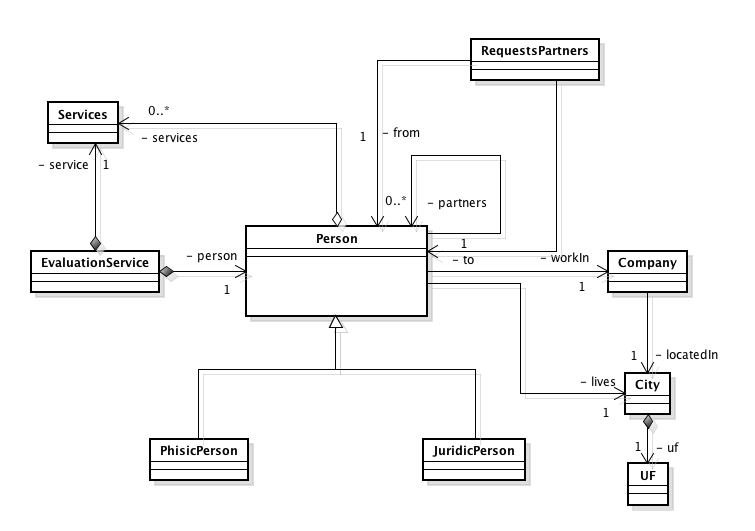
\includegraphics[scale=0.45]{./imagens/modelo-dominio-inicial.png}}
	\caption[Modelo de domínio inicial]
	{Modelo de domínio inicial. \textbf{Fonte:} Elaborado pelos autores.}
	\label{fig:modelo_dominio_inicial}
\end{figure}

\par Nesta fase, também foram definidas todas as ações cujo usuário poderia realizar no sistema, por meio dos casos de uso, conforme a Figura~\ref{fig:caso_uso_unificado}.

\newpage
\begin{figure}[h!]
	\centerline{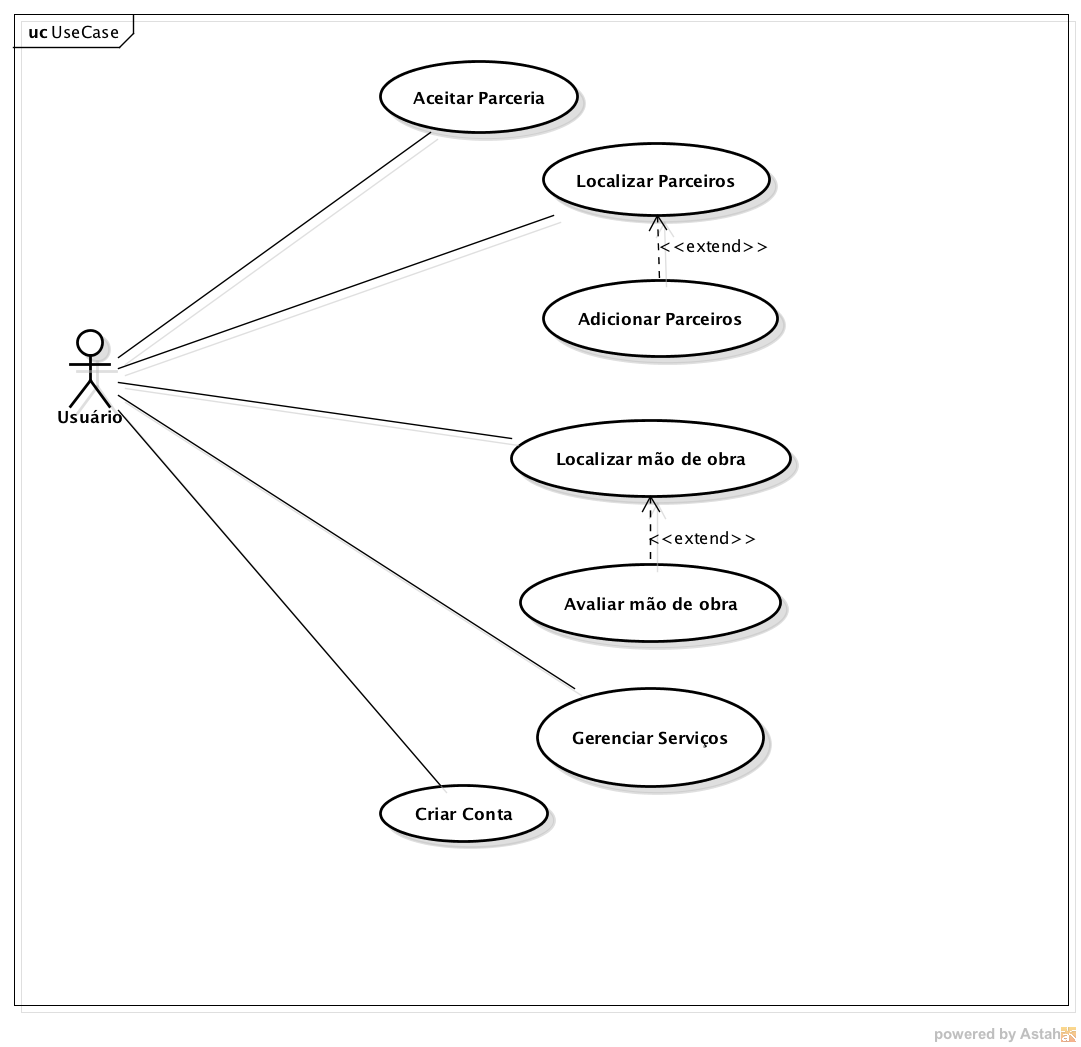
\includegraphics[scale=0.5]{./imagens/caso-de-uso-unificado.png}}
	\caption[Diagrama de caso de uso]
	{Diagrama de caso de uso. \textbf{Fonte:} Elaborado pelos autores.}
	\label{fig:caso_uso_unificado}
\end{figure}

% Removido após a pré-banca, pois, agora só haverá apenas um tipo de usuário (Ambos) e não mais provedor de serviço e contratante
%\newpage
%\begin{figure}[h!]
%	\centerline{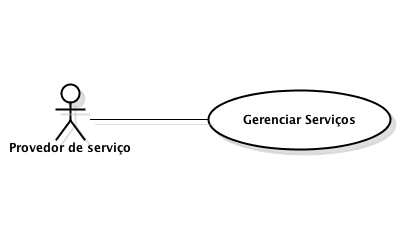
\includegraphics[scale=0.6]{./imagens/caso-de-uso-provedores-servico.png}}
%	\caption[Diagrama de caso de uso para provedores de serviços]
%	{Diagrama de caso de uso para provedores de serviços. \textbf{Fonte:} Elaborado pelos autores.}
%	\label{fig:caso_uso_provedor_servico_inicial}
%\end{figure}

%\begin{figure}[h!]
%	\centerline{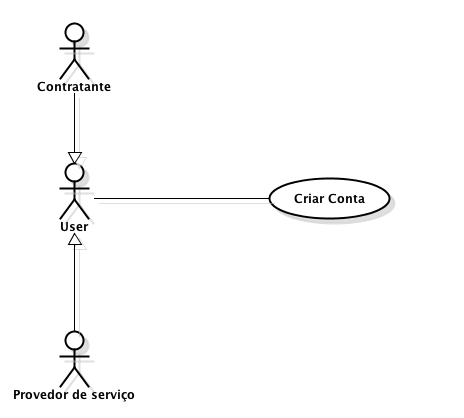
\includegraphics[scale=0.6]{./imagens/caso-de-uso-usuario.png}}
%	\caption[Diagrama de caso de uso para contratantes e provedores de serviços]
%	{Diagrama de caso de uso para contratantes e provedores de serviços. \textbf{Fonte:} Elaborado pelos autores.}
%	\label{fig:caso_uso_usuario_inicial}
%\end{figure}

\par Após definir os casos de uso, foram escritos os fluxos de eventos, para cada caso de uso. A seguir será apresentado o fluxo de eventos relacionado ao caso de uso ''Localizar parceiros'' por meio do Quadro~\ref{quad:fluxo_evento_localizar_parceiro}. Os demais fluxos de eventos são apresentados no Apêndice I em conjunto com os outros digramas deste trabalho.

% Conferir com o Márcio se os quadros serão removidos daqui e colocados nos apêndices depois só colar esta parte onde for inserida
%\newpage
%\begin{quadro}[h!]
%	\begin{fluxoDeEventos}
  \addTitle{Localizar Mão de obra}
  \addrow{Ator principal}{Contratante ou Ambos}
  \addrow{Ator secundário}{-}
  \addrow{Pré-condições}{O ator estar autenticado no sistema}
  \addrow{Pós-condições}{Provedores de serviço e suas respectivas mão de obras apresentadas ao ator.}
  
  \startBasicFlow{Ator} {Sistema}
  \addItemByColumnOne{O ator acessa a página para buscar o serviço por meio do menu “Busca” localizado no menu principal do sistema.}
  \addItemByColumnTwo{O sistema apresenta a página de busca de serviço e mão de obra.}
  
  \addItemByColumnOne{O ator informa qual a mão de obra que ele deseja pesquisar, por meio do campo “Buscar serviço”.}
  \addItemByColumnTwo{O sistema realiza uma busca pelo serviços que possuem o nome parecido com o nome do serviço informado pelo ator.ceiros que possuem maior probabilidade de se juntar a sua rede de parceiros.}
  
  \addItemByColumnOne{O ator seleciona o serviço a qual ele deseja que sejam pesquisados os provedores de serviço.}
  \addItemByColumnTwo{O sistema irá realizar a busca pela mão de obra solicitada pelo ator em sua base de dados, levando em consideração a rede de parceiros do ator, a empresa onde ele trabalha e a cidade onde o ator vive. Além é claro, da qualificação dos provedores de serviço. Após esta busca, o sistema apresentará uma página com a lista de prestadores de serviço que prestam tal mão de obra, ordenada pela credibilidade em sua rede de parceiros.}
  
  \addItemByColumnOne{O ator analisa a lista e seleciona a melhor opção a ele, clicando em sua imagem de perfil.}
  \addItemByColumnTwo{O sistema pesquisa todas as informações restantes do provedor de serviço, selecionado, pelo ator e apresenta uma página contendo todas as informações do provedor selecionado.}
   
  \startAlternativeFlow{Fluxo alternativo 1}
  \noAlternativeFlow{Não há fluxos alternativos}
\end{fluxoDeEventos}

%	\caption[Fluxo de eventos para o caso de uso ''localizar mão de obra'']
%	{Fluxo de eventos para o caso de uso ''localizar mão de obr''. \textbf{Fonte:} Elaborado pelos autores}
%	\label{quad:fluxo_evento_localizar_mao_de_obra}
%\end{quadro}

%\begin{quadro}[h!]
%	\begin{fluxoDeEventos}
  \addTitle{Avaliar Mão de obra}
  \addrow{Ator principal}{Contratante ou Ambos}
  \addrow{Ator secundário}{-}
  \addrow{Pré-condições}{O ator estar autenticado no sistema}
  \addrow{Pós-condições}{Mão de obra avaliada pelo ator}
  
  \startBasicFlow{Ator} {Sistema}
  \addItemByColumnOne{Após o item 6 do fluxo principal do fluxo de eventos “Localizar Mão de obra”. O ator clica no botão “Avaliar Serviço”.}
  \addItemByColumnTwo{O sistema apresenta o formulário de avaliação na mesma página para o ator.}
  
  \addItemByColumnOne{O ator preenche o formulário de avaliação da mão de obra e clica no botão “Salvar”.}
  \addItemByColumnTwo{O sistema registra a avaliação do cliente e apresenta uma mensagem de sucesso a ele.}
   
  \startAlternativeFlow{Fluxo alternativo 1}
  \noAlternativeFlow{Não há fluxos alternativos}
\end{fluxoDeEventos}

%	\caption[Fluxo de eventos para o caso de uso localizar mão de obra]
%	{Fluxo de eventos para o caso de uso localizar mão de obra. \textbf{Fonte:} Elaborado pelos autores}
%	\label{quad:fluxo_evento_avaliar_mao_de_obra}
%\end{quadro}

\newpage
\begin{quadro}[h!]
	\begin{fluxoDeEventos}
  \addTitle{Localizar Parceiros}
  \addrow{Ator principal}{Contratante ou Ambos}
  \addrow{Ator secundário}{-}
  \addrow{Pré-condições}{O ator estar autenticado no sistema}
  \addrow{Pós-condições}{Possíveis parceiro(s) apresentado(s) ao ator}
  
  

  \startBasicFlow{Ator} {Sistema}
  \addItemByColumnOne{O ator clica no menu “Rede de Parceiros” no menu principal localizado no menu principal do sistema.}
  \addItemByColumnTwo{O sistema apresenta a página contendo todos os parceiros ator e um campo para busca de novos parceiros.}
  
  \addItemByColumnOne{O ator informa o nome do parceiro que ele deseja encontrar no campo “Adicionar parceiros”.}
  \addItemByColumnTwo{O sistema pesquisa na sua base de dados os usuários que possuem aquele nome, e que por ventura, possuem algum tipo de ligação com os parceiros do ator, a fim de, tentar localizar os parceiros que possuem maior probabilidade de se juntar a sua rede de parceiros.}
  
  
  \startAlternativeFlow{Fluxo alternativo 1}
  \noAlternativeFlow{Não há fluxos alternativos}
\end{fluxoDeEventos}

	\caption[Fluxo de eventos para o caso de uso localizar parceiro]
	{Fluxo de eventos para o caso de uso localizar parceiro. \textbf{Fonte:} Elaborado pelos autores}
	\label{quad:fluxo_evento_localizar_parceiro}
\end{quadro}

%\newpage
%\begin{quadro}[h!]
%	\begin{fluxoDeEventos}
  \addTitle{Adicionar Parceiro}
  \addrow{Ator principal}{Contratante ou Ambos}
  \addrow{Ator secundário}{-}
  \addrow{Pré-condições}{O ator estar autenticado no sistema}
  \addrow{Pós-condições}{Parceiro(a) adicionado(a) a lista de parcerias do ator.}
  
  \startBasicFlow{Ator} {Sistema}
  \addItemByColumnOne{Após o item 4 do fluxo de eventos “Localizar Parceiros”. O ator clica na imagem de perfil do contratante a fim de, visualizar o perfil do possível novo parceiro.}
  \addItemByColumnTwo{O sistema realiza a busca das demais informações do contratante, cujo o ator selecionou para visualizar o perfil e apresenta a página de perfil dele ao ator.}
  
  \addItemByColumnOne{O ator visualiza o perfil do contratante e clique no botão “Adicionar Parceiro” para adicioná-lo  à sua lista de parceiros.}
  \addItemByColumnTwo{O sistema armazena esta requisição em sua base de dados, para aguardar a aprovação ou não do parceiro requisitado e apresenta uma mensagem de sucesso na requisição.}
 
  \startAlternativeFlow{Fluxo alternativo 1}
  \noAlternativeFlow{Não há fluxos alternativos}
\end{fluxoDeEventos}

%	\caption[Fluxo de eventos para o caso de uso adicionar parceiro]
%	{Fluxo de eventos para o caso de uso adicionar parceiro. \textbf{Fonte:} Elaborado pelos autores}
%	\label{quad:fluxo_evento_adicionar_parceiro}
%\end{quadro}

%\newpage
%\begin{quadro}[h!]
%	\begin{fluxoDeEventos}
  \addTitle{Aceitar Parceria}
  \addrow{Ator principal}{Contratante ou Ambos}
  \addrow{Ator secundário}{-}
  \addrow{Pré-condições}{O ator estar autenticado no sistema}
  \addrow{Pós-condições}{Novo(a) parceiro(a) adicionado(a) a lista de  parceiros do ator.}
  
  \startBasicFlow{Ator} {Sistema}
  \addItemByColumnOne{O ator acessa a página inicial do sistema personalizada a ele.}
  \addItemByColumnTwo{O sistema busca em sua base de dados todas as requisições de parcerias pendentes ao ator.}
  
  \addItemByColumnOne{Uma notificação push é apresentada ao ator no ícone “Novas Parcerias” do menu principal. Para visualizar a lista de requições pendentes, o ator deve passar o mouse sob este menu e um menu drop-down será apresentado ao ator contendo todas as requisições de parcerias.}
 
  \addEmptyColumn
  
  \addItemByColumnOne{Para responder a requisição o ator deve clicar no botão “confirmar” ou “cancelar” de cada uma das requisições da lista.}
  
  \addItemByColumnTwo{Ao clicar no botão “confirmar” o sistema confirma a parceria entre ambos os contratantes e apresenta uma mensagem de sucesso ao ator.}
  
  \startAlternativeFlow{Fluxo alternativo 1}
  \addItemByColumnOne{No item 4 do fluxo principal o ator clica no botão “cancelar” da requisição de parceria.}
  \addItemByColumnTwo{O sistema remove a requisição de parceria da sua base de dados, impedindo assim que a mesma requisição volte a ser apresentada ao ator.}
\end{fluxoDeEventos}

%	\caption[Fluxo de eventos para o caso de uso aceitar parceria]
%	{Fluxo de eventos para o caso de uso aceitar parceria. \textbf{Fonte:} Elaborado pelos autores}
%	\label{quad:fluxo_evento_aceitar_parceria}
%\end{quadro}

%\newpage
%\begin{quadro}[h!]
%	\begin{fluxoDeEventos}
  \addTitle{Gerenciar Serviços}
  \addrow{Ator principal}{Provedor de serviço}
  \addrow{Ator secundário}{-}
  \addrow{Pré-condições}{O ator estar autenticado no sistema}
  \addrow{Pós-condições}{Serviço atribuído ao ator.}
  
  \startBasicFlow{Ator} {Sistema}
  \addItemByColumnOne{O ator clica no menu “Serviço” apresentado na barra de menu principal do sistema.}
  \addItemByColumnTwo{O sistema apresenta a página contendo a lista de serviços prestados por ele, além do formulário para atrelar um novo serviço a ele.}
  
  \addItemByColumnOne{O ator começa a inserir o nome do serviço que deseja localizar.}
  \addItemByColumnTwo{O sistema realiza uma busca a fim de apresentar todas as opções possíveis de serviços anteriormente cadastradas no banco de dados , segundo o nome informado pelo ator.}
  
  \addItemByColumnOne{O ator seleciona o serviço que deseja atrelar a si mesmo por meio da lista de serviços apresentados e clica no botão “Adicionar”.}
  
  \addItemByColumnTwo{O sistema atrela o serviço ao ator com sucesso e apresenta uma mensagem de sucesso a ele.}
  
  \addItemByColumnOne{O ator lê a mensagem de sucesso.}
  \addEmptyColumn
  
  \startAlternativeFlow{Fluxo alternativo 1}
  \addItemByColumnTwo{No item 4 do fluxo principal, o sistema não localiza nenhum serviço em sua base de dados com o nome informado pelo ator e, portanto não apresenta nenhuma opção para seleção.}
  
  \addItemByColumnOne{O ator conclui o nome do serviço, caso seja necessário e clica no botão “Adicionar”.}
  \addItemByColumnTwo{O sistema verifica que o serviço não está registrado em sua base de dados, portanto, o cria e atrela ele ao ator. Após isto, apresenta uma mensagem de sucesso ao ator.}
  
  \addItemByColumnOne{O ator lê a mensagem de sucesso.}
  \addEmptyColumn
  
  
  \startAlternativeFlow{Fluxo alternativo 2}
  \addItemByColumnTwo{No item 6 do fluxo principal, o sistema realiza uma validação, a fim de evitar que o usuário atribua o mesmo serviço a si mesmo mais de uma vez.  Após isto, uma mensagem informando ao usuário sobre a falha é apresentada.}
  
  \addItemByColumnOne{O ator lê a mensagem de erro.}
  \addEmptyColumn
  
\end{fluxoDeEventos}

%	\caption[Fluxo de eventos para o caso de uso gerenciar serviços]
%	{Fluxo de eventos para o caso de uso gerenciar serviços. \textbf{Fonte:} Elaborado pelos autores}
%	\label{quad:fluxo_evento_gerenciar_servicos}
%\end{quadro}

%\newpage
%\begin{quadro}[h!]
%	\begin{fluxoDeEventos}
  \addTitle{Criar Conta}
  \addrow{Ator principal}{Usuário}
  \addrow{Ator secundário}{-}
  \addrow{Pré-condições}{}
  \addrow{Pós-condições}{Conta criada com sucesso}
  
  

  \startBasicFlow{Ator} {Sistema}
  \addItemByColumnOne{O ator acessa a página inicial do sistema.}
  \addItemByColumnTwo{O sistema apresenta a página de boas vindas ao usuário.}
  
  \addItemByColumnOne{O ator clica no menu “Criar conta” na barra de menu superior.}
  \addItemByColumnTwo{O sistema apresenta a tela para criar a nova conta.}
  
  \addItemByColumnOne{O ator preenche alguns campos relacionados aos seus dados pessoais e clica no botão “Próximo”.}
  \addItemByColumnTwo{O sistema armazena a nova conta e redireciona o ator para a página contendo o formulário correspondente ao segundo passo para concluir a criação de conta.}
  
  \addItemByColumnOne{O ator preenche alguns campos relacionados aos seus dados profissionais e clica no botão “Próximo”.}
  \addItemByColumnTwo{O sistema atualiza os dados da conta recém-criada e redireciona o ator para a página relacionada ao terceiro e último passo para criação da conta.}
  
  \addItemByColumnOne{O ator insere a sua imagem de perfil e clica no botão “Salvar”.}
  \addItemByColumnTwo{O sistema atualiza a conta recém-criada e redireciona o ator para a sua página inicial.}
  
  
  \startAlternativeFlow{Fluxo alternativo 1}
  \addItemByColumnTwo{No item 6 do fluxo principal, o sistema verifica que já existe um usuário com o mesmo e-mail.}
  
  \addItemByColumnTwo{O sistema apresenta uma mensagem de erro informando a situação ao ator.}
  
  \addItemByColumnOne{O ator lê a mensagem de erro.}
  \addItemByColumnTwo{O sistema mantém o estado atual da página, aguardando pela inserção de um e-mail válido.}
\end{fluxoDeEventos}

%	\caption[Fluxo de eventos para o caso de uso criar conta]
%	{Fluxo de eventos para o caso de uso criar conta. \textbf{Fonte:} Elaborado pelos autores}
%	\label{quad:fluxo_evento_criar_conta}
%\end{quadro}


\par Na segunda fase, análise e projeto preliminar, houve um refinamento dos requisitos levantados na fase anterior, aperfeiçoando as ações do usuário, por meio dos diagramas de casos de uso ou fluxos de eventos. Posterior a esta definição, foram desenvolvidos os diagramas de robustez, como demonstra a Figura~\ref{fig:diagrama_robustez_localizar_mao_de_obra}.

\newpage
\begin{figure}[h!]
	\centerline{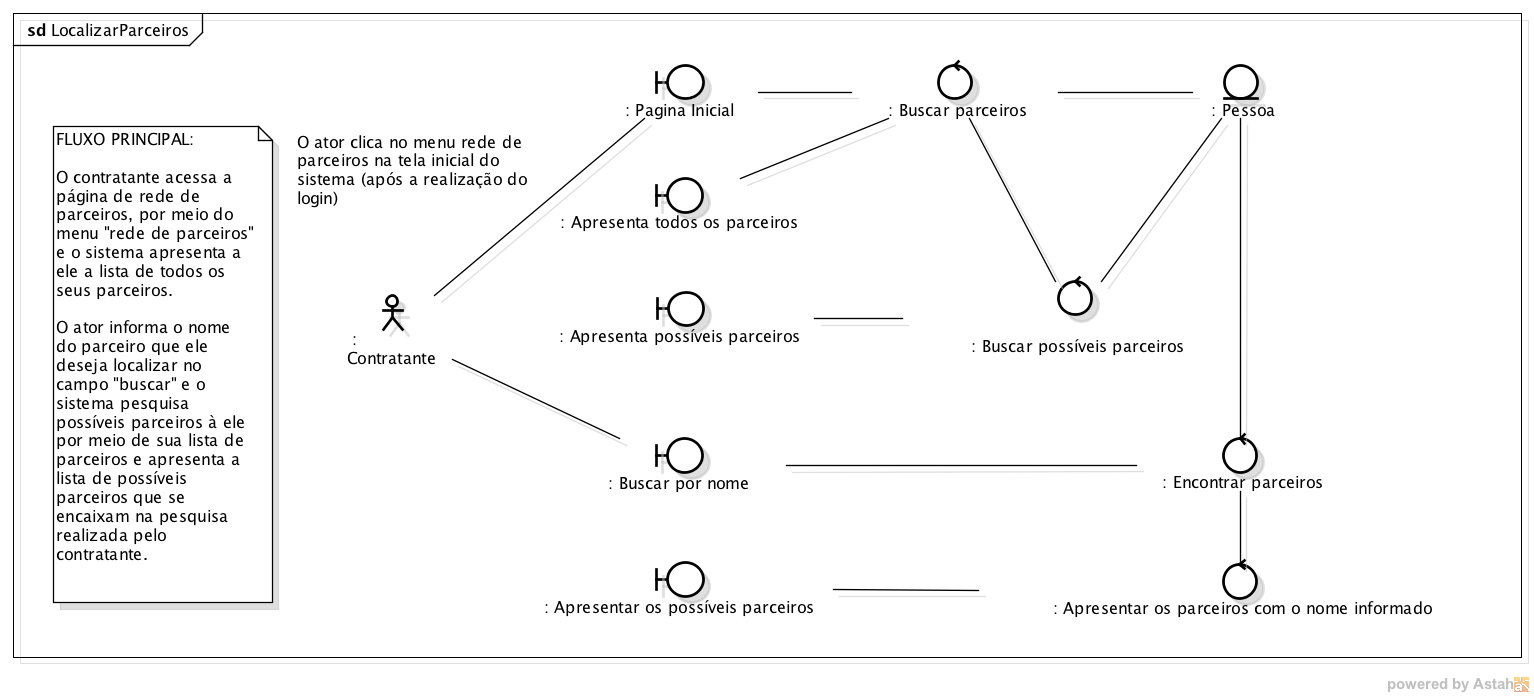
\includegraphics[scale=0.35]{./imagens/apendices/diagrama-robustez-localizar-parceiros.png}}
	\caption[Diagrama de robustez do caso de uso ''Localizar parceiros'']
	{Diagrama de robustez do caso de uso ''Localizar parceiros''. \textbf{Fonte:} Elaborado pelos autores.}
	\label{fig:diagrama_robustez_localizar_mao_de_obra}
\end{figure}

Em paralelo, foi atualizado o modelo de domínio, acrescentando os novos atributos identificados na segunda fase, conforme a Figura~\ref{fig:modelo_dominio_atualizado}.

\begin{figure}[h!]
	\centerline{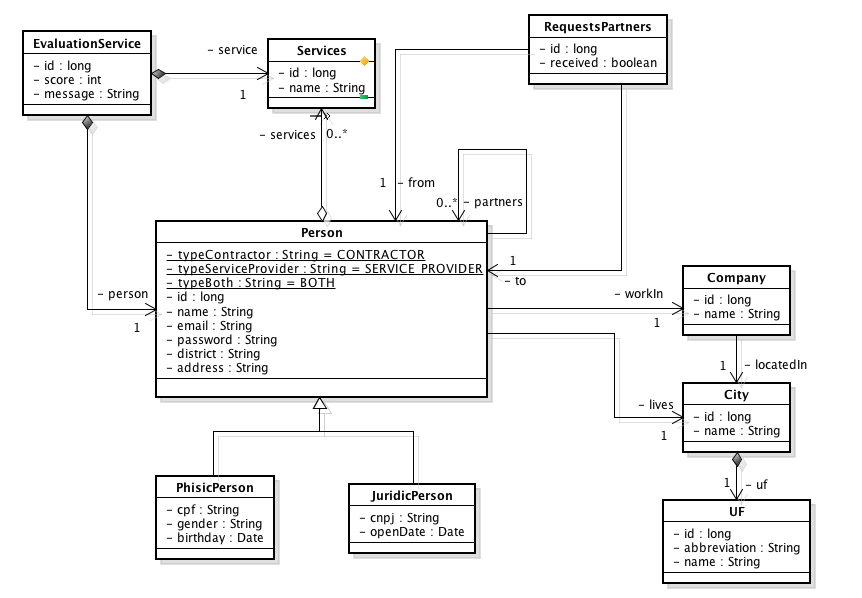
\includegraphics[scale=0.5]{./imagens/modelo-dominio-com-atributos.png}}
	\caption[Modelo de domínio atualizado]
	{Modelo de domínio atualizado. \textbf{Fonte:} Elaborado pelos autores.}
	\label{fig:modelo_dominio_atualizado}
\end{figure}

Com o modelo de domínio atualizado, foi feita a modelagem do banco de dados da aplicação, como apresenta a Figura~\ref{fig:modelo_dados_aplicacao}.

\begin{figure}[h!]
	\centerline{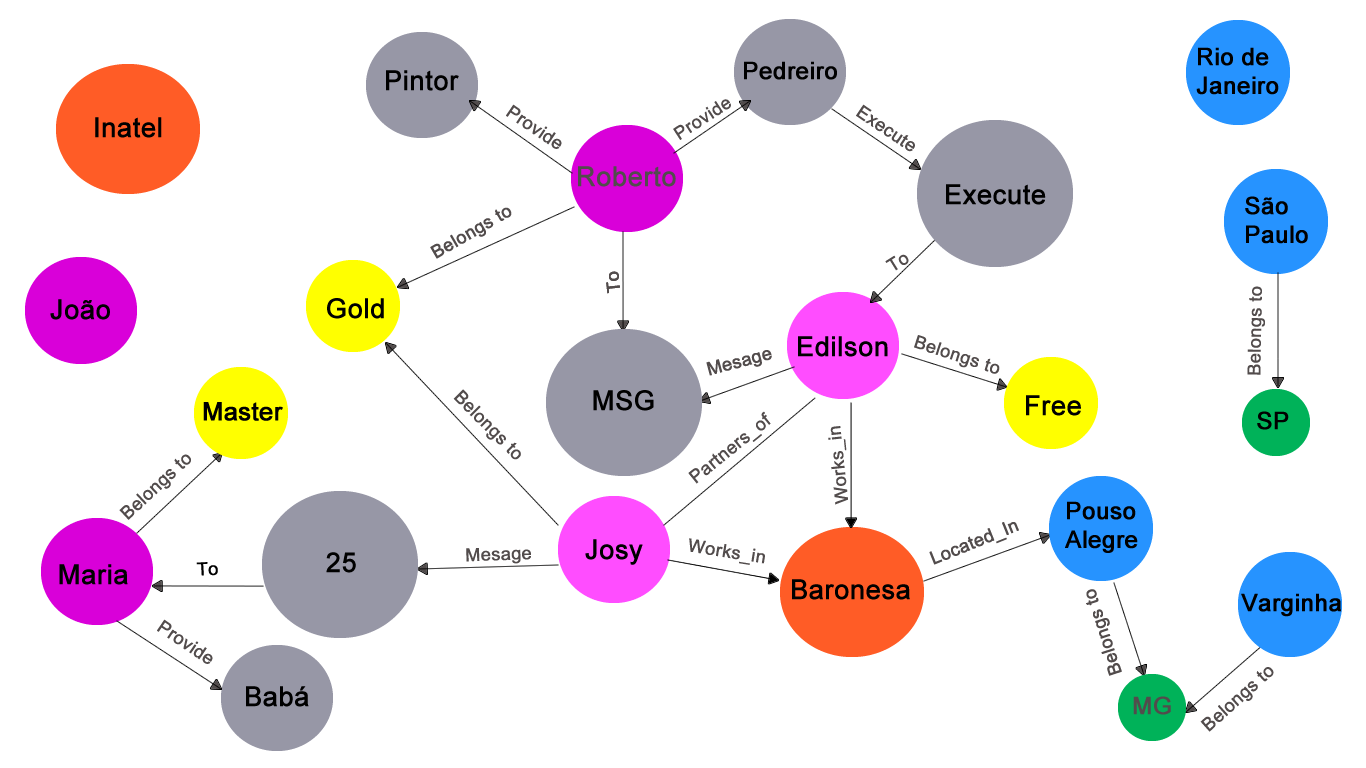
\includegraphics[scale=0.4]{./imagens/structure-all-nodes.png}}
	\caption[Modelo de dados da aplicação]
	{Modelo de dados da aplicação. \textbf{Fonte:} Elaborado pelos autores.}
	\label{fig:modelo_dados_aplicacao}
\end{figure} 

\par Na terceira fase, definida como projeto detalhado, foram criados os diagramas de sequência, tendo como base os casos de uso modelados na fase anterior. Esta fase tem como objetivo detalhar todo o funcionamento do \textit{software}, visando definir a melhor maneira de realizar sua implementação. A Figura~\ref{fig:diagrama_sequencia_localizar_parceiros} apresenta o diagrama de sequência do caso de uso ''Localizar parceiros''.

\newpage
\begin{figure}[h!]
	\centerline{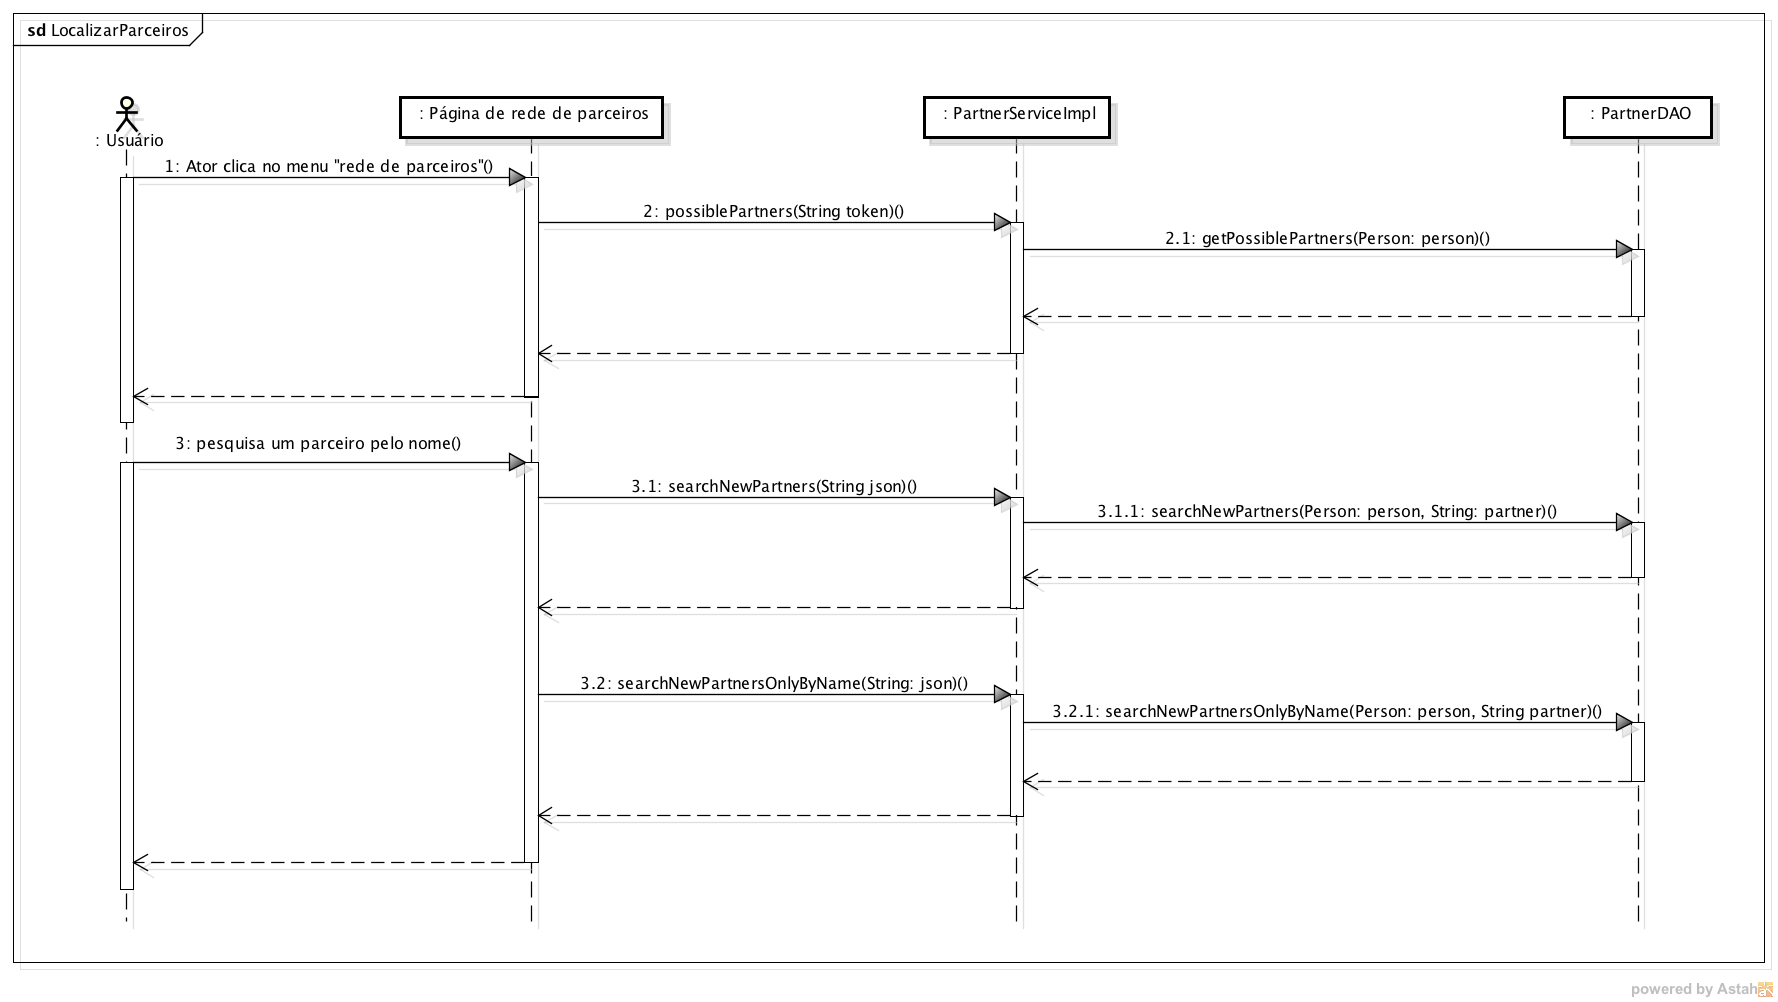
\includegraphics[angle=90,scale=0.4]{./imagens/diagrama-sequencia-localizar-novos-parceiros.png}}
	\caption[Diagrama de sequência do caso de uso ''Localizar parceiros'']
	{Diagrama de sequência do caso de uso ''Localizar parceiros''. \textbf{Fonte:} Elaborado pelos autores.}
	\label{fig:diagrama_sequencia_localizar_parceiros}
\end{figure}

\par Ainda na fase de projeto detalhado, após a modelagem dos diagramas de sequência, as operações encontradas nestes diagramas foram adicionadas ao modelo de domínio, em conjunto com as novas classes identificadas, gerando assim, o digrama de classes como mostra a Figura~\ref{fig:diagrama_classe}.

\begin{figure}[h!]
	\centerline{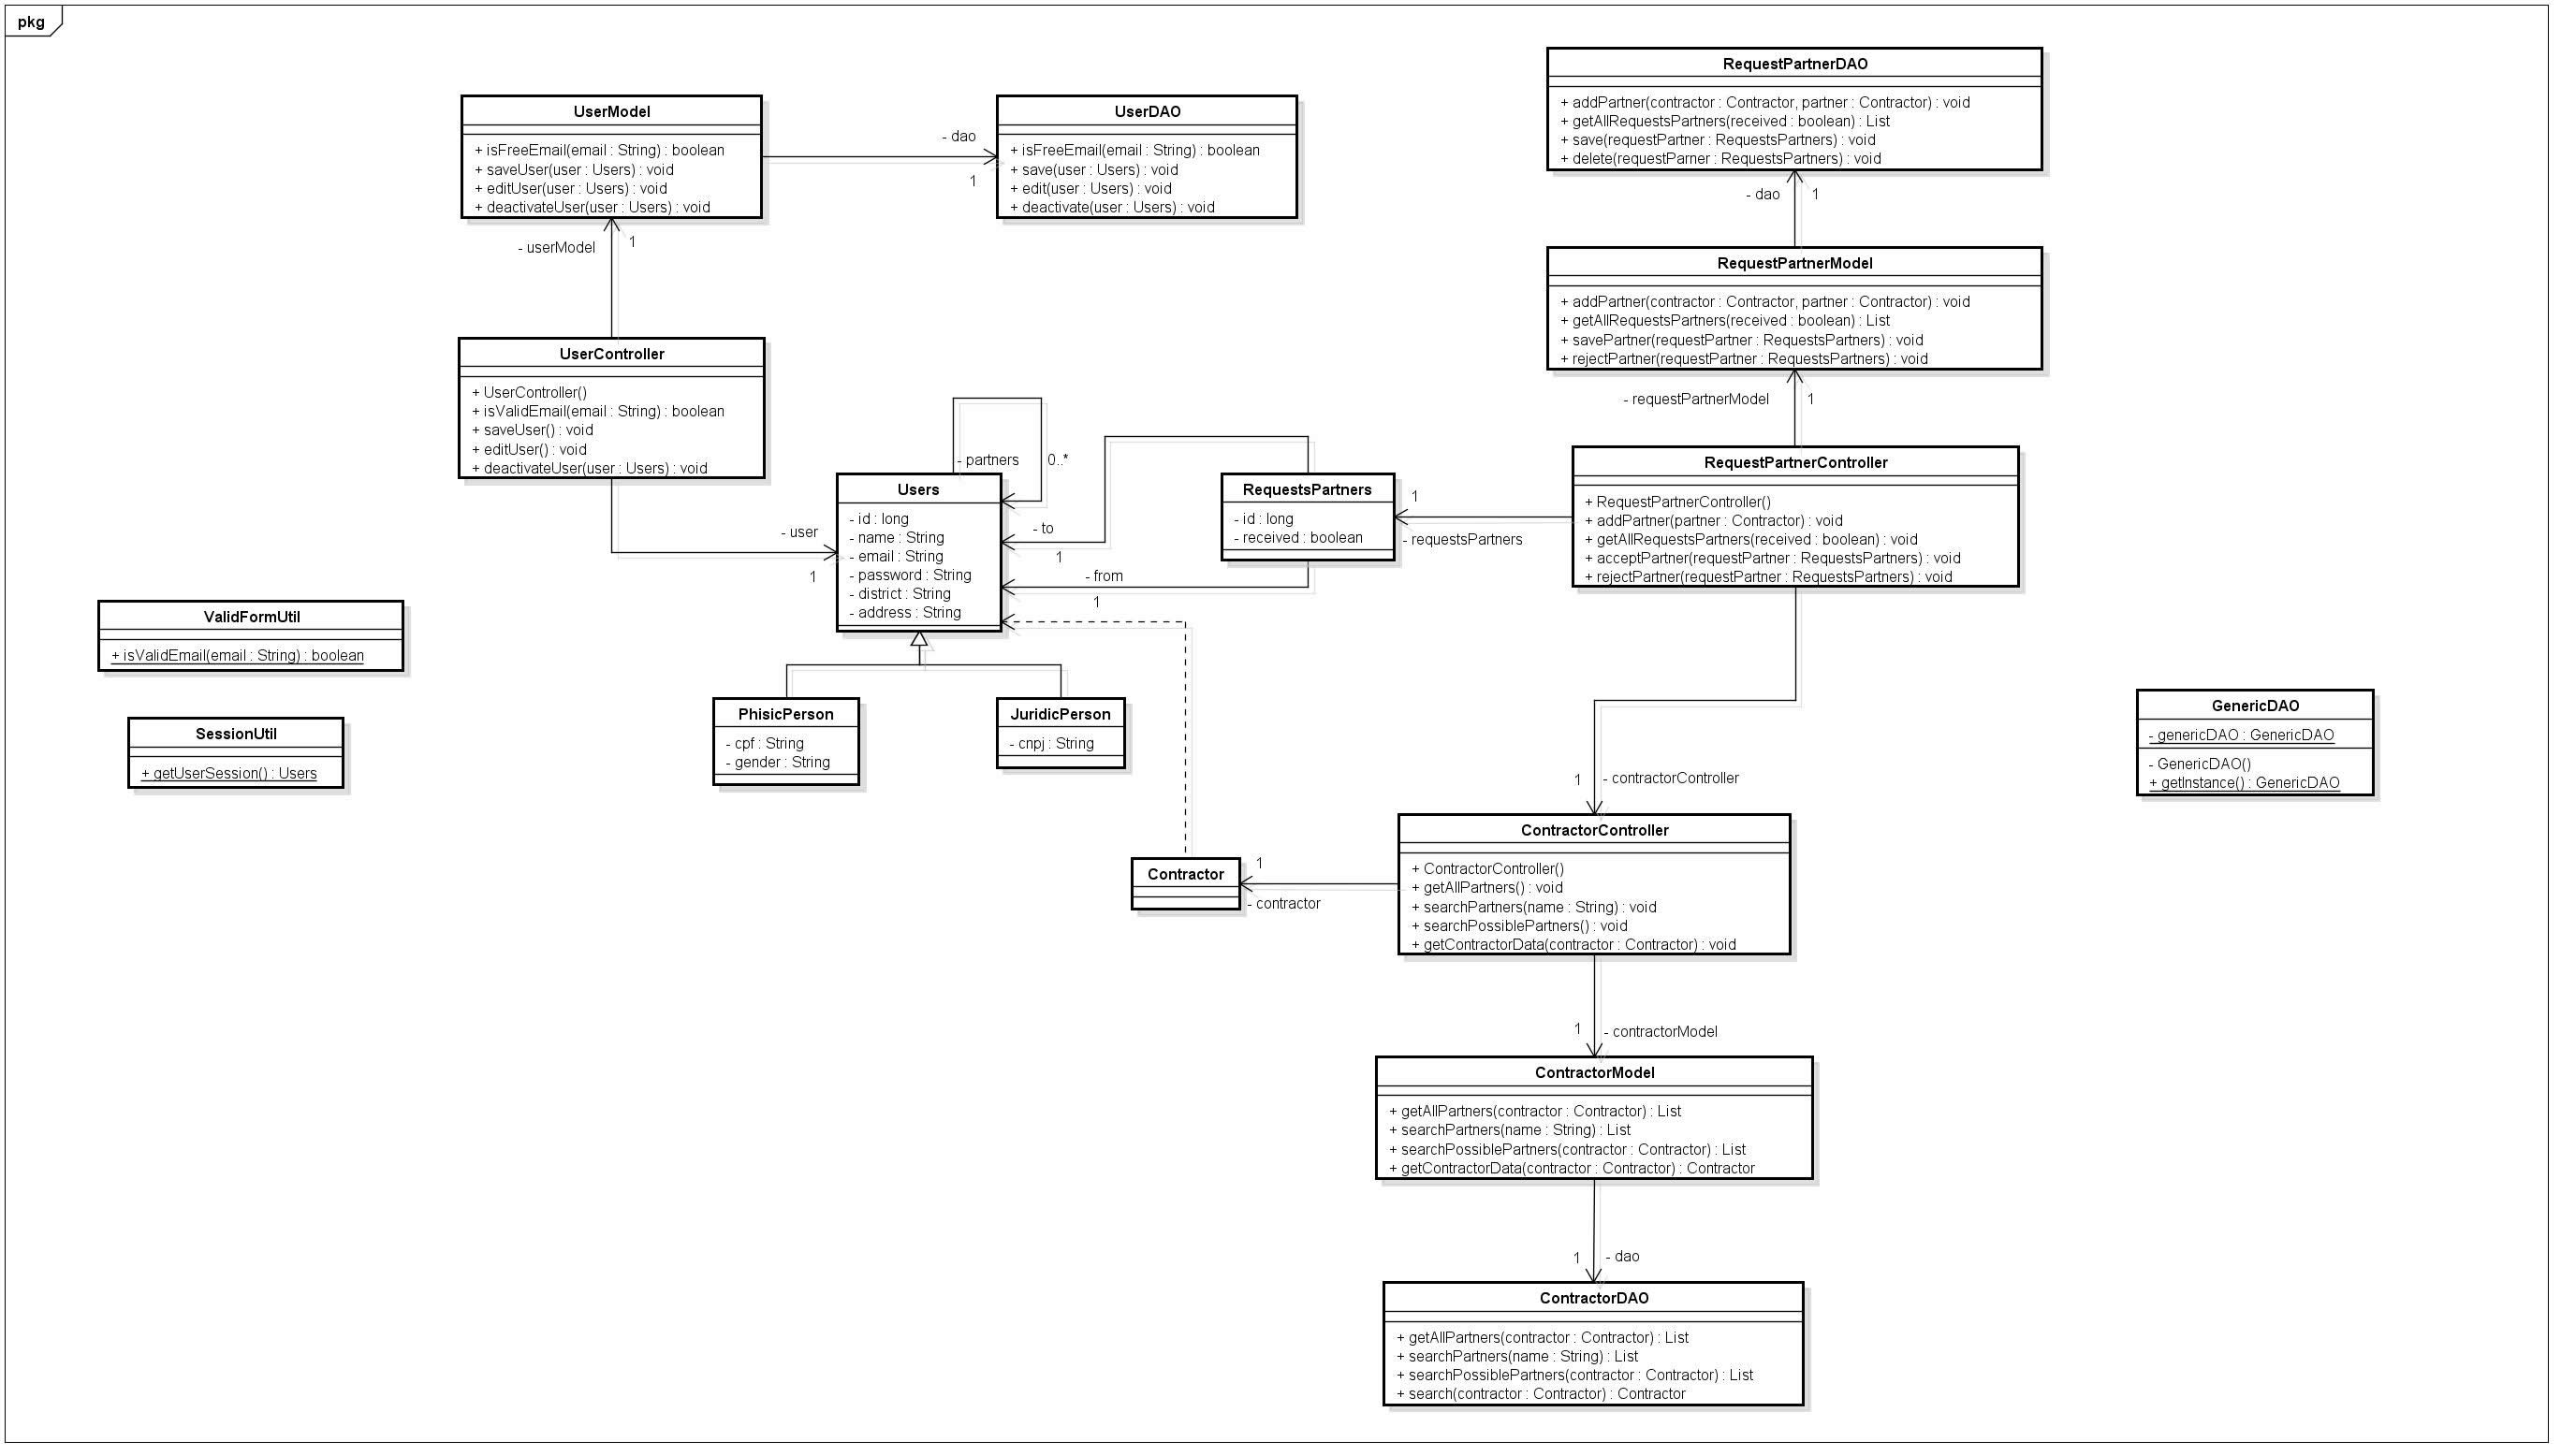
\includegraphics[angle=90,height=0.7\textheight,width=0.7\textwidth]{./imagens/classe.jpg}}
	\caption[Diagrama de classes]
	{Diagrama de classes \textbf{Fonte:} Elaborado pelos autores.}
	\label{fig:diagrama_classe}
\end{figure}

\newpage
\par Na quarta e última fase do ICONIX, denominada implementação, iniciou-se a preparação do ambiente, incluindo a instalação dos \textit{softwares} necessários para o desenvolvimento prático da aplicação. Essa preparação é abordada a seguir.


\section{Teoria dos Grafos}

\par A teoria dos grafos foi criada pelo matemático suiço Leonhard Euler no século XVIII com o propósito de solucionar um antigo problema, conhecido como as 7 pontes de \textit{Königsberg} \cite{harju_graph_theory}.

\par \textit{Königsberg}, atualmente conhecida como \textit{Kaliningrad}, era uma antiga cidade medieval cortada pelo rio \textit{Pregel} dividindo-a em 4 partes interligadas por 7 pontes. Ela era localizada na antiga Prússia, hoje, território Russo. O problema mencionado anteriormente consistia basicamente em atravessar toda a cidade, visitando todas as partes e utilizar todas as pontes desde que não repetisse uma das quatro partes ou uma das 7 pontes. A Figura 2 ilustra o problema mencionado.

% Imagem do problema das 7 pontes da teoria dos grafos
\begin{figure}[h!]
	\centerline{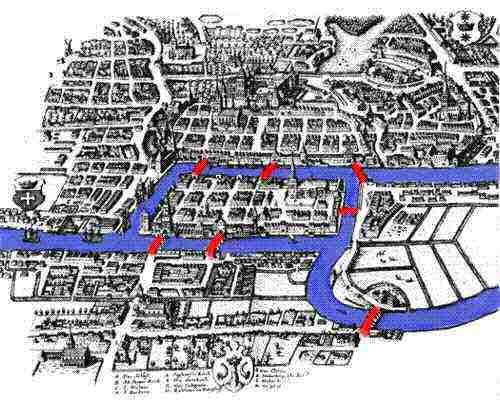
\includegraphics[height=0.26\textheight,width=0.8\textwidth]{./imagens/Konigsberg_7_bridges.jpg}}
	\caption[O problema das 7 pontes de \textit{Königsberg} ]
	{O problema das 7 pontes de \textit{Königsberg}. \textbf{Fonte:} \citeonline{paoletti_seven_bridges_konigsberg}}
	\label{fig:exemplo1}
\end{figure}

\par De acordo com \citeonline{bruggen_learning_neo4j}, para tentar solucionar o problema, Euler utilizou uma abordagem matemática ao contrário dos demais que tentaram utilizar a força bruta para solucionar tal problema, desenhando N números de diferentes possibilidades de rotas. Euler mudou o foco e passou a dar mais atenção ao número de pontes e não as partes da cidade. Por meio desta observação, foi possível perceber que realizar tal tarefa seria impossível, pois de acordo com sua teoria seria necessário possuir no mínimo mais uma ponte, uma vez que, o número de pontes era ímpar, não sendo possível realizar um caminho único e sem repetição. Desta forma, obteve-se a solução para este problema e criou-se o primeiro grafo no mundo.

\par \citeonline[p. 16]{rocha_algoritmos_particionamento_banco_dados_orientado_grafos} afirma que: 

\begin{citacao}
	um \textit{grafo G = (V,E)} consiste em um conjunto finito \textit{V} de vértices e um conjunto finito \textit{E} de arestas onde cada elemento \textit{E} possui um par de vértices que estão conectados entre si e pode ou não possuir um peso \textit{P}.
\end{citacao}

\par Esta é a definição formal de um grafo. A partir desta definição, é possível identificar, no problema mencionado anteriormente, os vértices que neste caso são as pontes e as arestas que por sua vez são as partes da cidade.

\par Segundo \citeonline{bondy_murty_graph_theory_with_applications}, muitas situações do mundo real podem ser descritas através de um conjunto de pontos conectados por linhas formando assim um grafo, como um centro de comunicações e seus \textit{links}, ou as pessoas e seus amigos, ou uma troca de emails entre pessoas, entre outras. Isto é possível pois, de acordo com \citeonline{rocha_algoritmos_particionamento_banco_dados_orientado_grafos}, existem muitos problemas atualmente que podem ser mapeados para uma estrutura genérica possibilitando assim utilizar a teoria de grafos para tentar solucioná-los, tais como: rotas geográficas, redes sociais, entre outros.

%BANCA_QUALIFICACAO. Comentado este parágrafo, porém o mesmo retornará para a banca de qualificação
\par A Figura 3 demostra de maneira visual um grafo, conforme ideia de \citeonline{bondy_murty_graph_theory_with_applications}, utilizando como exemplo o seguinte grafo \textit{G} = \{a, b, c, d, e, f, g, h\} e suas respectivas arestas \textit{E}$_g$ = \{(a, b), (a, h), (a, e), (b, f), (c, e), (c, d), (c, g), (d, e), (d, h), (d, g), (f, h)\}, sendo que os vértices serão representados por círculos e as arestas que os interligam por linhas.

%subscrito $_CARCTER_DESEJADO$

% Imagem do grafo simples - VOLTAR NA BANCA DE QUALIFICACAO
\begin{figure}[h!]
	\centerline{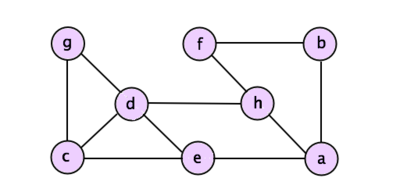
\includegraphics[scale=0.77]{./imagens/simple_graph.png}}
	\caption[Ilustração de uma representação gráfica de um simples grafo]
	{Ilustração de uma representação gráfica de um simples grafo. \textbf{Fonte:} \citeonline{rocha_algoritmos_particionamento_banco_dados_orientado_grafos}}
	\label{fig:exemplo1}
\end{figure}

%BANCA_QUALIFICACAO. Comentado este parágrafo, porém o mesmo retornará para a banca de qualificação
\par \citeonline{ruohonen_graph_theory} afirma que os grafos podem ser gerados com a possibilidade de permitir \textit{loops}\footnotemark[4] e arestas paralelas ou multiplas entre os vértices, obtendo um \textit{multigraph}. A Figura 4 ilustra um simples \textit{multigraph}.

\footnotetext[4]{\textit{loops} - Uma aresta que interliga o mesmo vértice.}

% Imagem de um multigraph - VOLTAR NA BANCA DE QUALIFICACAO
\begin{figure}[h!]
	\centerline{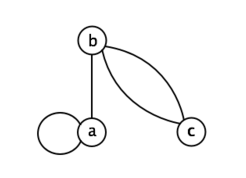
\includegraphics[scale=0.9]{./imagens/multigraph_example.png}}
	\caption[Ilustração de uma representação gráfica de um \textit{multigraph}]
	{Ilustração de uma representação gráfica de um \textit{multigraph}. \textbf{Fonte:} Adaptado de \citeonline{harju_graph_theory}}
	\label{fig:exemplo1}
\end{figure}

\newpage

%BANCA_QUALIFICACAO. Comentado este parágrafo, porém o mesmo retornará para a banca de qualificação
\par Para \citeonline{harju_graph_theory}, os grafos podem ser direcionados (\textit{dígrafo}) ou não direcionados. Os  direcionados são aqueles cujos vértices ligados a uma aresta são ordenados e permitem que uma aresta que conecta os vértices \textit{x} e \textit{y} seja representada apenas de uma forma, sendo ela \{x, y\} ou \{y, x\}, ao contrário dos não direcionados que, para este mesmo caso, podem ser representado por ambas as formas \cite{rocha_algoritmos_particionamento_banco_dados_orientado_grafos}. A Figura 5 demonstra um grafo direcionado.

% Imagem de um grafo direcionado - VOLTAR NA BANCA DE QUALIFICACAO
\begin{figure}[h!]
	\centerline{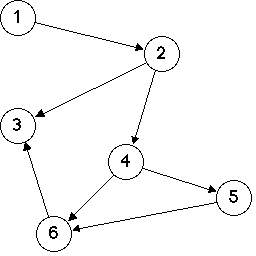
\includegraphics[scale=0.6]{./imagens/simple_digraph_graph.png}}
	\caption[Imagem de uma representação gráfica de um grafo direcionado]
	{Imagem de uma representação gráfica de um grafo direcionado. \textbf{Fonte:} \citeonline{robert_keller_acylic_graph}}
	\label{fig:exemplo1}
\end{figure}

Segundo \citeonline{harju_graph_theory}, os tipos de grafos são:

\begin{itemize}
	\item \textbf{grafo simples:} são aqueles grafos que não possuem \textit{loops} ou arestas paralelas;
	
	\item \textbf{grafo completo:} são aqueles em que, qualquer par de vértices são adjacentes;
	
	\item \textbf{subgrafos:} são pequenos grafos que em conjunto constituem um grafo maior.
	
	\item \textbf{grafos isomórficos:} dois grafos são isomórficos se, ambos possuírem a mesma estrutura de nós, e relacionamentos, exceto pelos identificadores de cada nó que podem ser diferentes, veja na Figura 6 um exemplo de dois grafos isomórficos \cite{harju_graph_theory}.
	
	\begin{figure}[h!]
		\centerline{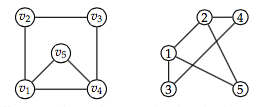
\includegraphics[scale=1]{./imagens/grafos_isomorficos.png}}
		\caption[Imagem de um grafo isomórfico]
		{Imagem de um grafo isomórfico. \textbf{Fonte:} \citeonline{harju_graph_theory}}
		\label{fig:exemplo1}
	\end{figure}
	
	\item \textbf{caminho (travessia):} é uma sequência de vértices \{v1, v2,...,vn\} conectados por meio de arestas. Exemplo: \{e1 = \{v1, v2\}, \{v1, v3\}..., \{vn, vm\}\};

	\item \textbf{grafo conexo:} são aqueles que, para qualquer par de vértices, há um caminho que os ligam;
	
	\item \textbf{grau do vértice:} é definido pela quantidade de arestas que se conectam ao vértice.
	
\end{itemize}

Para \citeonline{rocha_algoritmos_particionamento_banco_dados_orientado_grafos} existem várias formas de se representar um grafo computacionalmente utilizando diferentes estruturas de dados. Entretanto, a mais utilizada e simples é a matriz adjacência.

Uma matriz adjacência consiste em uma matriz contendo o mesmo número de linhas e colunas (\textit{n x n}). Veja na Figura 7 um exemplo de representação de um grafo utilizando esta estrutura.

\begin{figure}[h!]
	\centerline{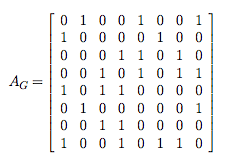
\includegraphics[scale=0.7]{./imagens/matriz_adjacencia.png}}
	\caption[Grafo representado por meio de uma matriz adjacência]
	{Grafo representado por meio de uma matriz adjacência. \textbf{Fonte:} \citeonline{rocha_algoritmos_particionamento_banco_dados_orientado_grafos}}
	\label{fig:exemplo1}
\end{figure}

Na Figura 7, as posições da matriz cujo o valor é igual a 1, definem que há uma aresta conectando os vértices, tornando-os assim, adjacentes. Caso o valor seja 0, os vértices não estão conectados entre si no grafo e, portanto, não são vértices adjacentes.

\par Este conteúdo teórico foi escolhido para ser utilizado neste trabalho pois este visa equacionar o problema relacionado à busca por mão de obra, através do modelo utilizado pelas redes sociais. Isto é possível pois, como mencionado anteriormente por meio desta teoria, é possível descrever várias situações do mundo real e como ela é muito bem aplicada à redes sociais, inclusive grandes empresas desta área já a utilizam. Devido a esses motivos, a teoria dos grafos foi utilizada para auxiliar no desenvolvimento deste trabalho.



\section{Tecnologias}

\par Nesta seção serão abordadas as linguagens de programação e as tecnologias que serão utilizadas para o desenvolvimento deste trabalho.

\subsection{Banco de dados}

\par A expressão ''Banco de dados'' teve origem a partir do termo inglês \textit{Databanks}, que foi substituído, mais tarde, pela palavra \textit{Databases} (Base de dados)  por possuir um significado mais apropriado \cite {setzer_silva_banco_dados_aprenda_o_que_sao_melhore_conhecimento}.

\par De acordo com \citeonline{date_introducao_sistemas_bancos_dados}, um banco de dados é uma coleção de dados persistentes, usada pelos sistemas de aplicação em uma determinada empresa. Sendo assim, um banco de dados é um local onde são armazenados os dados necessários para manter as atividades de determinadas organizações.

\par Um banco de dados possui, implicitamente, as seguintes propriedades: representa aspectos do mundo real; é uma coleção lógica de dados que possuem um sentido próprio e armazena dados para atender uma necessidade específica. O tamanho do banco de dados pode ser variável, desde que ele atenda às necessidades dos interessados em seu conteúdo \cite{elmasri_navathe_sistemas_banco_dados}.

%\subsubsection{Tipos de bancos de dados}

\par A escolha do banco de dados que será utilizado em um projeto é uma decisão importante e que deve ser tomada na fase de planejamento, pois determina características da futura aplicação, como a integridade dos dados, o tratamento de acesso de usuários, a forma de realizar uma consulta, o desempenho. Portanto, essa decisão deve ser bem analisada, levando em consideração o tipo de software e no ambiente de produção que será utilizado.

\par A seguir, são demonstrados os principais modelos de banco de dados, abordando suas características.

\subsection{Banco de dados relacionais}

\par O modelo de banco de dados relacional foi introduzido em 1970, por Edgar Frank Codd, em uma publicação com o título: “A relational model of data for large shared data banks”, na revista \textit{Association for Computing Machinery} (ACM). Essa publicação demonstrou como tabelas podem ser usadas para representar objetos do mundo real e como os dados podem ser armazenados para os objetos. Neste conceito, a integridade dos dados foi levada mais a sério do que em qualquer modelo de banco de dados antes visto. A partir desta publicação, surgiram muitos bancos de dados que passaram a utilizar este conceito e se tornaram muito utilizados no desenvolvimento de aplicações
\cite{matthew_stones_beginning_databases_with_postgresql}.

\par Segundo \citeonline{matthew_stones_beginning_databases_with_postgresql}, o conceito é baseado na teoria reacional da matemática e por isso há uma grande flexibilidade para o acesso e a manipulação de dados que são gravados no banco de dados. Utilizam-se técnicas simples, como normalização na modelagem do banco de dados, criando várias tabelas relacionadas, que servem como base para consultas usando uma linguagem de consulta quase padronizada, a \textit{Structured Query Language} – SQL\footnotemark[5].

\footnotetext[5]{SQL: \textit{Structured Query Language} - Linguagem para consultas e alterações em bancos de dados.}

% Pode voltar mais a frente no TCC quando for necessário aumentar esta parte
%\par Ainda segundo \citeonline{matthew_stones_beginning_databases_with_postgresql}, um banco de dados relacional contém relações (tabelas) com atributos (colunas) e tuplas (linhas). Todo atributo possui um tipo de dado predefinido, uma tupla representa um conjunto de dados contendo um valor para cada atributo da linha e as tabelas são relacionadas através de chaves.

\par A utilização de banco de dados relacionais geraram a necessidade de dividir os dados agregados utilizados na aplicação em várias relações conforme as regras da normalização. Para recuperar o mesmo dado agregado são necessárias consultas utilizando \textit{joins}\footnotemark[6], uma operação que, dependendo do tamanho das relações e da quantidade de dados, pode não ser tão eficiente. Nos casos em que se precisa obter uma resposta rápida de um sistema, isso se torna uma desvantagem \cite{sadalage_fowler_nosql_distilled_brief_guide}.

\footnotetext[6]{\textit{joins} - função utilizada para realizar a junção entre tabelas, facilitando a busca em bancos de dados relacionais.}

% Pode voltar mais a frente no TCC quando for necessário aumentar esta parte
%\par A figura 6 ilustra bem esta situação de divisão de um agregado e as suas relações resultantes.

% Imagem do exemplo de join - PODE VOLTAR MAIS TARDE NO TCC (Confirmar com o Márcio)
%\begin{figure}[h!]
	%\centerline{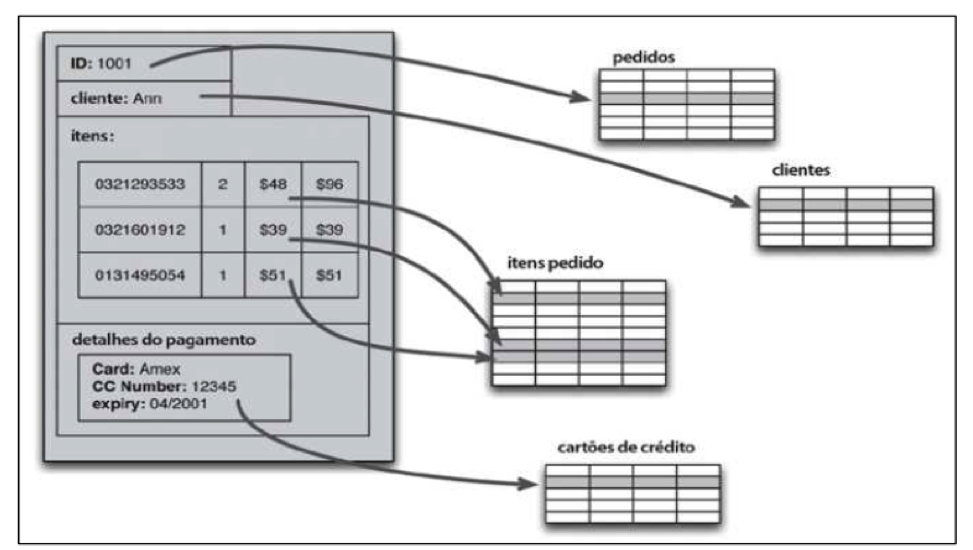
\includegraphics[scale=0.8]{./imagens/example_joins_sadalage.png}}
	%\caption[Agregado no UI é conjunto de várias tuplas de várias tabelas]
	%{Agregado no UI é conjunto de várias tuplas de várias tabelas. \textbf{Fonte:} \citeonline[p. 29]{sadalage_fowler_nosql_distilled_brief_guide}}
	%\label{fig:exemplo1}
%\end{figure}

\par Este foi um dos fatores determinantes que motivaram a criação de novas tecnologias, a fim de sanar o problema mencionado acima. A partir desta motivação, foram desenvolvidos novos modelos de banco de dados, que serão apresentados a seguir.


\subsection{Banco de dados NoSQL}

\par A expressão NoSQL é um termo não definido claramente. Ela foi ouvida pela primeira vez em 1998 como um nome para o banco de dados relacional de Carlo Strozzi, que assim o nomeou por não fornecer uma SQL-API. O mesmo termo foi usado como nome do evento NoSQL Meetup em 2009, que teve como objetivo a discussão sobre sistemas de bancos de dados distribuídos.

\par Devido a explosão de conteúdos na \textit{web} no início do século XXI, houve-se a necessidade de substituir os bancos de dados relacionais por bancos que oferececem maior capacidade de otimização e performance, a fim de suportar o grande volume de informações eminentes a esta mudança \cite{bruggen_learning_neo4j}.

\par \citeonline[p. 27]{rocha_algoritmos_particionamento_banco_dados_orientado_grafos} afirma que NoSQL é "um acrônimo para Not only SQL, indicando que esses bancos não usam somente o recurso de Structured Query Language (SQL), mas outros recursos que auxiliam no armazenamento e na busca de dados em um banco  não relacional".

\par Segundo \citeonline{bruggen_learning_neo4j}, os banco de dados NoSQL podem ser categorizados de 4 maneiras diferentes, são elas: \textit{Key-Value stores}\footnotemark[6], \textit{Column-Family stores}\footnotemark[7], \textit{Document stores}\footnotemark[8] e \textit{Graph Databases}\footnotemark[9].

\footnotetext[6]{\textit{Key-Value stores} - armazenamento por um par de chave e valor.}

\footnotetext[7]{\textit{Column-Family stores} - armazenamento por colunas e linhas.}

\footnotetext[8]{\textit{Document stores} - armazenamento em arquivos.}

\footnotetext[9]{\textit{Graph Databases} - banco de dados orientado a grafo.}
%\begin{itemize}
%\item \textit{Key-Value stores};
%\item \textit{Column-Family stores};
%\item \textit{Document stores};
%\item \textit{Graph Databases}.
%\end{itemize}

\par De acordo com \citeonline{bruggen_learning_neo4j}, o banco de dados orientado a grafo (\textit{graph database}) pertence a categoria NoSQL, contudo, ele possui particularidades que o torna muito diferente dos demais tipos de bancos de dados NoSQL. A seguir, será descrito com maiores detalhes o banco de dados orientado a grafos Neo4j.


\subsection{Neo4j}

\par O Neo4j foi criado no início do século XXI por desenvolvedores que queriam resolver um problema em uma empresa de mídias. Porém, eles não obtiveram êxito ao tentar resolver tal problema utilizando as tecnologias tradicionais, portanto, decidiram arriscar e criar algo novo. A princípio, o Neo4j não era um sistema de gerenciamento de banco de dados orientado a grafos como é conhecido nos dias atuais. Ele era mais parecido com uma \textit{graph library} (biblioteca de grafo) em que as pessoas poderiam usar em seus projetos \cite{bruggen_learning_neo4j}.

\par De acordo com \citeonline{bruggen_learning_neo4j}, inicialmente ele foi desenvolvido para ser utilizado em conjunto com alguns bancos de dados relacionais como MySQL e outros, com a intenção de criar uma camada de abstração dos dados em grafos. Mas com o passar dos anos, os desenvolvedores decidiram tirar o Neo4j da estrutura dos bancos relacionais e criar sua própria estrutura de armazenamento em grafos.

\par O Neo4j, como vários outros, também é um projeto de sistema de gerenciamento de banco de dados NoSQL de código fonte aberto.

\par Segundo \citeonline{robinson_webber_eifrem_graph_databases}, os bancos de dados orientados a grafos possuem como diferencial a sua performance, agilidade e flexibilidade. Entretanto, a performance é o que mais se destaca entre eles, pois, a maneira como eles armazenam e realizam buscas no banco de dados é diferente dos bancos de dados convencionais. Primeiramente, esse tipo de banco de dados não utiliza tabela; ele armazena os dados em vértices e arestas. Isso permite realizar buscas extremamente velozes através de \textit{traversals} (travessias), uma vez que estas implementam algoritmos para otimizar tais funcionalidades, evitando assim o uso de \textit{joins} complexos, tornando-o tão veloz.

\par \citeonline[p. 2]{neo4j_team_manual} afirma que:

\begin{citacao}
	\textit{A single server instance can handle a graph of billions of nodes and relationships. When data throughput is insufficient, the graph database can be distributed among multiple servers in a high availability configuration.}\footnotemark[11]
\end{citacao}

\footnotetext[11]{Um único servidor pode manipular um grafo de bilhões de nós e relacionamentos. Quando a taxa de transferência de dados é insuficiente, o banco de dados orientado a grafo pode ser distribuído entre vários servidores mantendo a mesma velocidade de processamento.}

\par Com estas informações, é possível mensurar o quanto o Neo4j pode ser rápido e robusto, sendo possível, até mesmo distribuí-lo a fim de obter uma melhor configuração, organização e facilidade de manutenção.

%BANCA_QUALIFICACAO. Comentado este parágrafo, porém o mesmo retornará para a banca de qualificação
\par Segundo \citeonline{neo4j_team_manual}, o banco de dados Neo4j é composto por nós (vértices), relacionamentos (arestas) e propriedades. Os relacionamentos são responsáveis por organizar os nós e ambos podem possuir seus atributos. É possível realizar as buscas e/ou alterações no Neo4j de duas formas diferentes. Sendo a primeira através da API \textit{Cypher Query Language}, que é uma \textit{query language} para banco de dados orientado a grafos muito próxima da linguagem humana, cuja descrição completa será apresentada a seguir. A segunda é o \textit{framework\footnotemark[12] Traversal} que utiliza a API \textit{Cypher} internamente para navegar pelo grafo.

\footnotetext[12]{\textit{Framework} - Abstração que une códigos comuns entre vários projetos de software, a fim de obter uma funcionalidade genérica.}


\citeonline{rocha_algoritmos_particionamento_banco_dados_orientado_grafos} afirma que o Neo4j permite criar mais de um relacionamento entre o mesmo par de vértices, desde que estes sejam de tipos distintos. Isso possibilita navegar pelos vértices do grafo de forma mais rápida devido a esses diferentes tipos de arestas, o que torna possível implementar o algoritmo de busca desejado. A Figura~\ref{fig:grafo_simples_neo4j} exemplifica um simples grafo utilizando um banco de dados Neo4j.


\begin{figure}[h!]
	\centerline{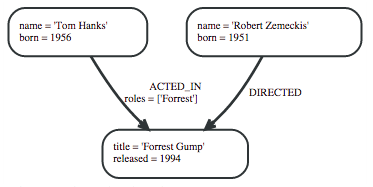
\includegraphics[scale=0.8]{./imagens/simple_graph_neo4j.png}}
	\caption[Exemplo simples de um grafo no Neo4j]
	{Exemplo simples de um grafo no Neo4j. \textbf{Fonte:} \citeonline{neo4j_team_manual}}
	\label{fig:grafo_simples_neo4j}
\end{figure}

\newpage
%BANCA_QUALIFICACAO. Comentado este parágrafo, porém o mesmo retornará para a banca de qualificação
\par Há duas formas de executar o Neo4j, segundo \citeonline{robinson_webber_eifrem_graph_databases}. A primeira é conhecida como \textit{Server} e a segunda \textit{Embedded}. O modo \textit{Server} é utilizado principalmente em \textit{web-service} em conjunto com a API REST, este será aplicado neste trabalho. Já no modo \textit{Embedded} o banco de dados é executado embarcado à aplicação Java.

%BANCA_QUALIFICACAO. Comentado este parágrafo, porém o mesmo retornará para a banca de qualificação
\par Conforme \citeonline{neo4j_team_manual}, o Neo4j possui suporte as transações ACID (com atomicidade, consistência, isolamento e durabilidade).

O Neo4j é distribuído em duas versões sendo elas a \textit{Entreprise} e a \textit{Community}. A primeira possui um tempo de avaliação de 30 dias e após esse tempo, é necessário comprar uma licença para continuar a utilizá-lo. Como diferencial essa versão possui ferramentas para o gerenciamento do banco de dados, incluindo melhorias relacionadas à escalabilidade. A segunda versão é disponibilizada gratuitamente sem data limite de expiração, contudo, ela não possui os recursos mencionados anteriormente que estão presentes na versão \textit{Enterprise}, mas é muito utilizada para fins didáticos e para pequenos projetos, aplicando-se perfeitamente a este projeto \cite{neo4j_team_manual}.

\par Por ser um banco de dados orientado a grafo bastante robusto, seguro e possuir uma documentação de fácil entendimento, além, é claro, de possuir um baixo custo de implantação devido a sua licença \textit{open source}, esse banco de dados foi escolhido para ser utilizado neste trabalho.


\subsection{\textit{Cypher Query Language}}

\par O \textit{Cypher Query Language} é uma linguagem para consultas em banco de dados orientado a grafo específica para o banco Neo4j. Ela foi criada devido à necessidade de manipular os dados e realizar buscas em grafos de uma forma mais simples, uma vez que, não é necessário escrever \textit{traversals} (\textit{travessias}) para navegar pelo grafo \cite{neo4j_team_manual}.


\par \citeonline{robinson_webber_eifrem_graph_databases}, afirmam que, o \textit{Cypher} foi desenvolvido para ser uma \textit{query language} que utiliza uma linguagem formal, permitindo a um ser humano entendê-la. Desta forma, qualquer pessoa envolvida no projeto é capaz de compreender as consultas realizadas no banco de dados. 

%BANCA_QUALIFICACAO. Comentado este parágrafo, porém o mesmo retornará para a banca de qualificação
\par Segundo \citeonline{neo4j_team_manual}, o \textit{Cypher} foi inspirado em uma série de abordagens e construído sob algumas práticas já estabelecidas, inclusive a SQL. Por este motivo, é possível notar que ele utiliza algumas palavras reservadas que são comuns na SQL como \textit{WHERE} e \textit{ORDER BY}.

%BANCA_QUALIFICACAO. Comentado este parágrafo, porém o mesmo retornará para a banca de qualificação
\par De acordo com \citeonline{neo4j_team_manual}, o \textit{Cypher} é composto por algumas cláusulas, dentre elas, se destacam:

%%BANCA_QUALIFICACAO. Comentado estes itens, porém os mesmos retornarão para a banca de qualificação
\begin{itemize}
	\item \textit{START}: Define um ponto inicial para a busca, este ponto pode ser um relacionamento ou um nó.
	\item \textit{MATCH}: Define o padrão de correspondência entre os nós. Para identificar um nó é necessário incluí-lo entre um par de parenteses, e os relacionamentos são identificados um hífen e um sinal de maior ou menor.
	\item \textit{CREATE}: Utilizado para criar nós e relacionamentos no grafo.
	\item \textit{WHERE}: Define um critério de busca.
	\item \textit{RETURN}: Define quais nós, relacionamentos e propriedades de ambos devem ser retornados da \textit{query} realizada. 
	\item \textit{SET}: Utilizado para editar as propriedades de um nó ou de um relacionamento.
	\item \textit{UNION}: Possibilita juntar o resultado de duas ou mais consultas.
	\item \textit{FOREACH}: Realiza uma ação de atualização para cada elemento na lista.
\end{itemize} 

\par Outras \textit{Query Languages} existem, inclusive com suporte ao Neo4j, porém devido as vantagens apresentadas acima, somada ao fato que ele possui uma curva de aprendizagem menor e é excelente para lhe oferecer uma base a respeito de grafos,  este \textit{framework} será utilizado para realizar as tarefas de manipulação dos dados no banco de dados.


\subsection{Java}

\par Segundo \citeonline{schildt_java_complete_reference}, a primeira versão da linguagem Java foi criada por James Gosling, Patrick Naughton, Chris Warth, Ed Frank e Mike Sheridan na \textit{Sun Microsystems} em 1991 e denominada "Oak" cujo seu principal foco era a interatividade com a TV. Mais tarde, em 1995, a \textit{Sun Mycrosystems} renomeia esta linguagem e anuncia publicamente a tecnologia Java, focando nas aplicações \textit{web}, que em pouco tempo e devido à grande ascensão da internet, cresceu e se mantém em constante evolução até os dias atuais.

\par De acordo com a \citeonline{oracle_about_java_technology}, a tecnologia Java não é apenas uma linguagem, mas também uma plataforma, que teve como modelo uma outra linguagem, o C++ que, por sua vez foi derivada da linguagem C. O C++ e o Java possuem em comum o conceito de orientação a objetos. O que permite a esta linguagem utilizar recursos como: generalização (herança), implementação, polimorfismo, entre outras. Tais funcionalidades permitem ao desenvolvedor escrever códigos reutilizáveis, a fim de facilitar o desenvolvimento do projeto.

\par Para \citeonline{schildt_java_complete_reference}, o paradigma de orientação a objetos foi criado devido às limitações que o conceito estrutural apresentava quando era utilizado em projetos de grande porte, dificultando o desenvolvimento e manutenção dos mesmos. Este paradigma possibilita ao desenvolvedor aproximar o mundo real ao desenvolvimento de \textit{software}, deixando os objetos do mundo real semelhantes a seus respectivos objetos da computação, possibilitando ao desenvolvedor modelar seus objetos de acordo com suas necessidades \cite{tcc_univas_faria_aspectj_programacao_orientada_aspecto_java}.

Segundo \citeonline{schildt_java_complete_reference}, o recurso denominado generalização (herança) permite ao desenvolvedor criar uma classificação hierárquica de classes. Além disso, é possível escrever uma classe genérica contendo comportamentos comum, e as demais classes, cujo tais comportamentos também serão aplicados a ela, somente precisa generalizar esta classe.

O polimorfismo se refere ao princípio da biologia em que um organismo pode ter diferentes formas ou estados. Este mesmo princípio, também pode ser aplicado à programação orientada a objeto. Desta forma, é possível definir comportamentos que serão compartilhadas entre as classes e suas respectivas sub classes, além de comportamentos próprios cujo apenas as sub classes possuem. Com isto, o comportamento pode ser diferente de acordo com a forma e/ou o estado do objeto \cite{polymorphism_oracle}.

\par Retomando a ideia da \citeonline{oracle_about_java_technology}, uma das vantagens da tecnologia Java sob as demais é o fato de ela ser multiplataforma, possibilitando ao desenvolvedor escrever o código apenas uma vez e este, ser executado em qualquer plataforma inclusive em hardwares com menor desempenho. Isto é possível, pois, para executar um programa em Java é necessário possuir uma \textit{Java Virtual Machine} - JVM\footnotemark[12] - instalada no computador. A JVM compreende e executa apenas \textit{bytecodes}\footnotemark[13] e estes por sua vez são obtidos através do processo de compilação do código escrito em Java.

%Nota a respeito da sigla JVM
\footnotetext[12]{JVM: \textit{Java Virtual Machine} - Máquina virtual utilizada pela linguagem Java para execução e compilação de \textit{softwares} desenvolvidos em Java.}

%Nota a respeito de bytecodes
\footnotetext[13]{\textit{Bytecode} é o código interpretado pela JVM. Ele é obtido por meio do processo de compilação de um programa java como mencionado anteriormente.}

\par Todo programa que utiliza Java necessita passar por algumas etapas essenciais. Conforme ilustrado na figura 9, o código é escrito em arquivo de texto com extensão \texttt{.java}, após isto ele será compilado e convertido para um arquivo com extensão \texttt{.class}, cujo o texto é transformado em \textit{bytecodes}. Este arquivo com extensão \texttt{.class} é interpretado pela JVM que é responsável por executar todo o código do programa.

\newpage
% Imagem do Processo de compilação do Java
\begin{figure}[h!]
	\centerline{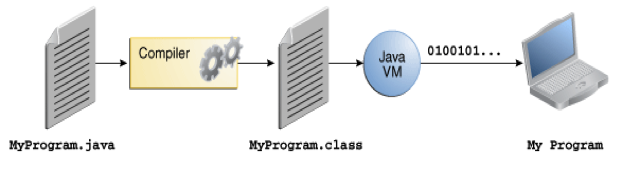
\includegraphics[scale=1]{./imagens/processo_compilacao_java.png}}
	\caption[Uma visão geral do processo de desenvolvimento de software.]
	{Uma visão geral do processo de desenvolvimento de software. \textbf{Fonte:} \citeonline{oracle_about_java_technology}}
	\label{fig:exemplo1}
\end{figure}

\par Por todas as vantagens descritas acima, será empregado o uso desta tecnologia neste projeto.


\subsection{Tomcat 7}

\par O Tomcat é uma aplicação \textit{container}, capaz de hospedar aplicações \textit{web} baseadas em Java. A princípio ele foi criado para executar \textit{servlets}\footnotemark[15] e \textit{JavaServer Pages} - JSP\footnotemark[16]. Inicialmente ele era parte de um sub projeto chamado \textit{Apache-Jakarta}, porém, devido ao seu sucesso ele passou a ser um projeto independente, e hoje, é responsabilidade de um grupo de voluntários da comunidade \textit{open source} do Java \cite{vukotic_goodwill_apache_tomcat_7}.

\footnotetext[15]{\textit{Servlet} - Programa Java executado no servidor, semelhante a um \textit{applet}.}

\footnotetext[16]{JSP: \textit{JavaServer Pages} - Tecnologia utilizada para desenvolver páginas interativas utilizando Java \textit{web}.}

\par Segundo a \citeonline{apache_about_tomcat}, o Tomcat é um software que possui seu código fonte aberto e disponibilizado sob a \textit{Apache License Version 2}. Isto o fez se tornar uma das aplicações \textit{containers} mais utilizadas por desenvolvedores.

\par \textit{Containers} são aplicações que são executadas em servidores e possuem a capacidade de hospedar aplicações desenvolvidas em Java \textit{web}. O servidor ao receber uma requisição do cliente, entrega esta ao \textit{container} no qual é distribuído. O \textit{container}, por sua vez, entrega ao \textit{servlet} as requisições e respostas HTTP\footnotemark[17] e inicia os métodos necessários do \textit{servlet} de acordo com o tipo de requisição realizada pelo cliente \cite{basham_sierra_bates_use_cabeca_servlets_jsp}.

\footnotetext[17]{HTTP: \textit{Hypertext Transfer Protocol} - Protocolo de transferência de dados mais utilizado na rede mundial de computadores.}

%BANCA_QUALIFICACAO. Comentado este parágrafo, porém o mesmo retornará para a banca de qualificação
\par \citeonline{brittain_darwin_apache_tomcat_2nd_edition} afirmam que o Tomcat foi desenvolvido utilizando a linguagem de programação Java, sendo necessário possuir uma versão do \textit{Java Runtime Environment} - JRE\footnotemark[18] - instalada e atualizada para executá-lo.

\footnotetext[18]{JRE: \textit{Java Runtime Environment} - Conjunto de ferramentas necessárias para a execução de aplicações desenvolvidas na linguagem Java.}
%BANCA_QUALIFICACAO. Comentado este parágrafo, porém o mesmo retornará para a banca de qualificação
\par De acordo com  \citeonline{laurie_laurie_apache_the_definitive_guide}, o Tomcat é responsável por realizar a comunicação entre a aplicação e o servidor Apache\footnotemark[19] por meio do uso de \textit{sockets}.

\footnotetext[19]{Apache - Servidor cujo aplicação Tomcat é executada.}

\par Assim como outros \textit{containers}, \citeonline{basham_sierra_bates_use_cabeca_servlets_jsp} afirmam que o Tomcat oferece gerenciamento de conexões \textit{sockets}, suporta \textit{multithreads}, ou seja, ele cria uma nova \textit{thread} para cada requisição realizada pelo cliente e gerencia o acesso aos recursos do servidor, além de outras tarefas.

\par O Tomcat, em especial, foi escolhido para ser utilizado neste trabalho, pois o objetivo é desenvolver uma aplicação \textit{web} e para hospedá-la em um servidor, uma aplicação \textit{container} se faz necessária. Por este motivo, e somado a sua facilidade de configuração, além das vantagens acima descritas tal decisão foi tomada.


\subsection{\textit{Web Service} REST}

A definição computacional de serviço é um \textit{software} que disponibiliza sua funcionalidade por meio de uma interface denominada contrato de serviço \cite{erl_soa_with_rest}.

\textit{Web Service} de acordo com \citeonline{marzulo_soa_na_pratica}, é uma materialização da ideia de um serviço que é disponibilizado na internet, e que, devido a isso, pode ser acessado em qualquer lugar do planeta e por diferentes tipos de dispositivos. Para ter acesso aos serviços que o \textit{Web Service} disponibiliza, o solicitante envia requisições de um tipo anteriormente definido e recebe respostas síncronas ou assíncronas.

\citeonline{marzulo_soa_na_pratica} afirma que, a implementação de um \textit{Web Service} é relativamente simples, uma vez que, há inúmeras ferramentas que facilitam a implementação do mesmo. Outro fator que permite a um \textit{Web Service} ser mais dinâmico é possuir uma estrutura interna fracamente acoplada, permitindo, assim, mudanças em suas estruturas sem afetar a utilização pelo cliente.

\citeonline{erl_soa_with_rest} afirmam que o REST\footnotemark[20], é uma das várias implementações utilizadas para criar serviços. Outra implementação também muito conhecida é: a SOAP\footnotemark[21] em conjunto com o WSDL\footnotemark[22], cujo responsabilidade é definir o contrato dos serviços.

\footnotetext[20]{REST: \textit{Representational State Transfer} - Tecnologia utilizada por \textit{web services}}

\footnotetext[21]{SOAP: \textit{Simple Object Access Protocol} - Tecnologia utilizada por \textit{web services} anteriores aos \textit{Web services} REST.}

\footnotetext[22]{WSDL: \textit{Web Service Description Language} - Padrão de mercado utilizado para descrever \textit{Web Services}.}

O primeiro\textit{Web Service} REST foi criado por Roy Fielding no ano 2000 na universidade da California. Ele foi criado para suceder o tecnologia SOAP, a fim de facilitar o uso de tal tecnologia. \cite{ibm_web_service}.

Segundo \citeonline{oracle_web_service}, na arquitetura do REST os dados e as funcionalidades são considerados recursos e ambos são acessados por meio de  URIs\footnotemark[23]. Ele funciona baseado no protocolo HTTP, portanto, já possui os mecanismos de segurança, cabeçalhos e respostas presentes neste protocolo.

\footnotetext[23]{URI: \textit{Uniform Resource Identifier} - \textit{Link} completo para acessar um determinado recurso.}

Para \citeonline{ibm_web_service}, o \textit{Web service} REST segue quatro princípios básicos. São eles: 

\begin{itemize}
	\item utiliza os métodos HTTP explicitamente;
	\item é orientado à conexão;
	\item expõe a estrutura de diretório por meio das URIs;
	\item trabalha com -\textit{Extensible Markup Language} - XML\footnotemark[24], \textit{Javascript Object Notation} - JSON\footnotemark[25] - ou ambos.
\end{itemize}

\footnotetext[24]{XML: \textit{Extensible Markup Language} - Tecnologia utilizada para transferência de dados, configuração, entre outras atividades.}

\footnotetext[25]{JSON: \textit{Javascript Object Notation} - Notação de objetos via Javascript, porém seu uso não é restrito apenas ao Javascript.}

Essa tecnologia foi selecionada para ser utilizada neste trabalho, pois a forma de acesso ao banco de dados Neo4j utiliza uma API REST fornecida pelo próprio Neo4j,

\subsection{HTML 5}

Segundo \citeonline{w3c_html_fundamentals}, \textit{Hypertext Markup Language}  - HTML\footnotemark[26] - é a linguagem usada para descrever o conteúdo das páginas \textit{web}. Ela utiliza marcadores denominados \textit{tags} para identificar aos navegadores de internet como eles devem interpretar tal documento.

\footnotetext[26]{HTML: \textit{Hypertext Markup Language} - Linguagem usada para descrever o conteúdo das páginas \textit{web}.}

\citeonline{silva_css_3} afirma que o HTML foi criado única e exclusivamente para ser uma linguagem de marcação e estruturação de documentos (páginas) \textit{web}. Portanto, não cabe a ele definir os aspectos dos componentes como cores, espaços, fontes, etc.

\citeonline{w3c_html_fundamentals} afirma que a primeira versão do HTML foi criada no ano de 1991 pelo inventor da \textit{web}, Tim Berners-Lee. A partir desta versão, o HTML foi e continua em constante atualização e hoje se encontra na sua oitava versão. As oito versões são: HTML, HTML +, HTML 2.0, 3.0, 3.2, 4.0, 4.01 e a versão atual é a 5.

Ao longo dos anos e da evolução propriamente dita do HTML, novas \textit{tags} foram criadas, padrões adotados, e claro, novas versões foram criadas, até que, em maio de 2007  o \textit{World Wide Web Consortium} - W3C\footnotemark[27] - confirma a decisão de voltar a trabalhar na atual versão do HTML, também conhecida por HTML 5 \cite{w3c_html_fundamentals}.

\footnotetext[27]{W3C:  \textit{World Wide Web Consortium} - Consórcio internacional formado por empresas, instituições, pesquisadores, desenvolvedores e público em geral, com a finalidade de elevar a web ao seu 	potencial máximo.}

\citeonline{silva_html5} afirma que em novembro daquele mesmo ano o W3C publicou uma nota contendo uma série de diretrizes que descrevem os princípios a serem seguidos ao desenvolver utilizando o HTML 5 em algumas áreas. Tais princípios permitiram a esta versão maior segurança, maior compatibilidade entre navegadores e interoperabilidade entre diversos dispositivos.

Por estes motivos, somado ao fato de que ao utilizar essa tecnologia é possível obter uma maior flexibilidade no desenvolvimento das páginas \textit{web}, o HTML foi selecionado para ser utilizado neste trabalho, em conjunto com outras tecnologias cujas descrições serão apresentadas nas próximas seções.

\subsection{CSS 3}

\citeonline{silva_css_3} afirma que a principal função do \textit{Cascading Style Sheet} - CSS\footnotemark[28] - é definir como os componentes anteriormente estruturados nos documentos \textit{web}, por meio do HTML, devem ser apresentados ao usuário.

\footnotetext[28]{CSS: \textit{Cascading Style Sheet} - Documentos que definem estilos aos componentes da página \textit{web}.}

Para \citeonline{w3c_css_definition}, o CSS é "\textit{a simple mechanism for adding style (e.g., fonts, colors, spacing) to Web documents}\footnotemark[29]".

\footnotetext[29]{O CSS é um simples mecanismo para adicionar estilo, como: fontes, cores, espaços para os documentos \textit{Web}.}

Tim Berners-Lee inicialmente escrevia as estilizações de seus documentos \textit{web}, mesmo que de forma simples e limitada, nos próprios documentos HTML. Isto se deve ao fato de, ele acreditar que tal função deveria ser realizada pelos navegadores. Entretanto, em 1994 a primeira proposta de criação do CSS surgiu e, em 1996, a primeira versão do CSS denominada CSS 1 foi lançada como recomendação do W3C \cite{silva_css_3}.

De acordo com \citeonline{silva_css_3}, atualmente o CSS possui quatro versões, são elas: A CSS 1, a 2, a 2.1 e atualmente a 3, que foi utilizada para o desenvolvimento deste trabalho.

Há três formas de incorporar o CSS em seu documento web segundo \cite{silva_css_3}, são elas: 

\begin{itemize}
	\item \textbf{\textit{Inline}:} É possível aplicar o estilo diretamente ao componente desejado, por meio do uso da propriedade \texttt{style} do componente HTML. Como é apresentado na Figura 10;
	
	\newpage
	\begin{figure}[h!]
		\centerline{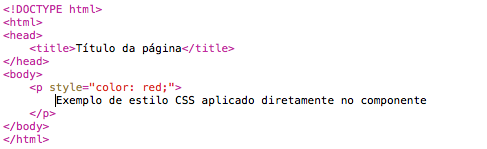
\includegraphics[scale=0.8]{./imagens/example_css_inline.png}}
		\caption[Exemplo de inclusão do estilo CSS inline]
		{Exemplo de inclusão do estilo CSS inline. \textbf{Fonte:} Elaborado pelos autores.}
		\label{fig:exemplo1}
	\end{figure}
	
	\item \textbf{Incorporado:} Outra forma, é escrever todo CSS referente ao  documento \textit{web} dentro da \textit{tag} \texttt{style} do documento HTML. Para tanto, esta \textit{tag} deve ser inserida entre o início e o fim da \textit{tag} \texttt{head} do documento. Como é apresentado na Figura 11;
	
	\begin{figure}[h!]
		\centerline{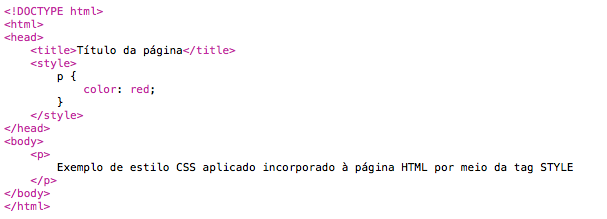
\includegraphics[scale=0.8]{./imagens/example_css_incorpored.png}}
		\caption[Exemplo de inclusão do estilo CSS incorporado à página HTML]
		{Exemplo de inclusão do estilo CSS incorporado à página HTML. \textbf{Fonte:} Elaborado pelos autores.}
		\label{fig:exemplo1}
	\end{figure}
	 
	\item \textbf{Externo:} A última forma, é criar um arquivo externo com extensão \texttt{.css} e definir todas as regras de estilização do documento \textit{web} neste arquivo. Desta forma, para vincular tal arquivo a um documento HTML específico será necessário utilizar a \textit{tag} \texttt{link} entre o início e o fim da \textit{tag} \texttt{head} do documento, como apresentado na Figura 12;
	
	\newpage
	\begin{figure}[h!]
		\centerline{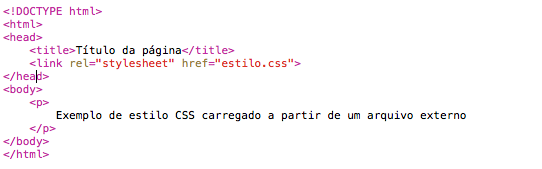
\includegraphics[scale=0.8]{./imagens/example_external_css.png}}
		\caption[Exemplo de inclusão do estilo CSS a partir de um arquivo externo]
		{Exemplo de inclusão do estilo CSS a partir de um arquivo externo. \textbf{Fonte:} Elaborado pelos autores.}
		\label{fig:exemplo1}
	\end{figure}
	
\end{itemize}

O CSS 3 será utilizado neste trabalho, pois, ele permite definir estilos aos componentes das páginas \textit{web} e possui recursos que não são existem em suas versões anteriores, o que nos permite desenvolver páginas mais atrativas com menos recursos.

\subsection{Javascript}

\citeonline{javascript_diego_leonard} afirmam que o Javascript foi criado e lançado pela Netscape em 1995, em conjunto com o navegador de internet Netscape Navigator 2.0. A partir deste lançamento, as páginas \textit{web} passaram a ganhar vida com a possibilidade de implementar um mínimo de dinamicidade. Isto se deve ao modo como a linguagem acessa e manipula os componentes do navegador. Contudo, ela pode ser utilizada em diferentes dispositivos como \textit{smartphones, smart tv}, entre outros, não limitando-se apenas a navegadores de internet.

O Javascript é uma linguagem de programação para \textit{web}. A maioria dos sites usa essa linguagem, inclusive todos os navegadores mais modernos, vídeo games, \textit{tablets}, \textit{smart phones}, \textit{smart tvs} possuem interpretadores de \textit{Javascript}, o que a tornou, a linguagem de programação mais ambígua da história \cite{flanagan_javascript_definitive_guide}.

Segundo \citeonline{javascript_diego_leonard}, as semelhanças entre o Javascript e o Java se limitam apenas ao nome. A primeira linguagem não deriva da segunda, apesar de ambas compartilharem alguns conceitos e detalhes. O Javascript, por ser uma linguagem interpretada, é mais flexível que o Java, que, por sua vez, é uma linguagem compilada.

De acordo com \citeonline{flanagan_javascript_definitive_guide}, o Javascript possui 6 versões, sendo elas: 1.0, 1.1, 1.2, 1.3, 1.4 e a atual versão 1.5.

Para \citeonline{javascript_diego_leonard}, há duas maneiras de incluir e executar o código escrito em Javascript nos documentos HTML. A primeira é incluir o código Javascript entre as \textit{tags} \texttt{script} como mostra o Código~\ref{list:javascript_incorporado}. 

% Inserindo o código Javascript via listagem
\begin{lstlisting} [style=custom_HTML,caption={[Inclusão do código em Javascript incorporado ao HTML.]{Inclusão do código em Javascript incorporado ao HTML. \textbf{Fonte:} Elaborado pelos autores.}}, label=list:javascript_incorporado] 	
<!DOCTYPE html>
<html>
	<head>
		<title>Titulo da pagina</title>
	</head>
	<body>
		<script type="text/javascript">
			document.writeLine("Exemplo de codigo Javascript incorporado " +
								 "ao documento HTML por meio da TAG SCRIPT");
		</script>
	</body>
</html>
\end{lstlisting}

% Trocado de imagem para listagem
%\begin{figure}[h!]
%	\centerline{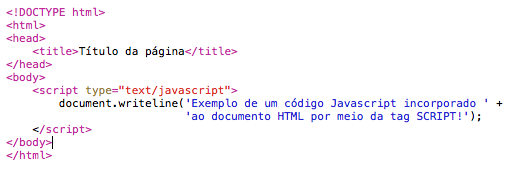
\includegraphics[scale=0.8]{./imagens/javascript_code.png}}
%	\caption[Exemplo de inclusão do código em Javascript incorporado ao HTML]
%	{Exemplo de inclusão do código em Javascript incorporado ao HTML. \textbf{Fonte:} Elaborado pelos autores.}
%	\label{fig:javascript_incorporado}
%\end{figure}

A segunda forma é incluir um arquivo externo com extensão \texttt{.js} através da mesma \textit{tag} \texttt{script}. Veja um exemplo de inclusão de um arquivo contendo códigos em Javascript no documento HTML no Código~\ref{list:javascript_externo}.

% Inserindo o código Javascript via listagem
\begin{lstlisting} [style=custom_HTML,caption={[Inclusão do código Javascript de um arquivo externo.]{Inclusão do código Javascript de um arquivo externo. \textbf{Fonte:} Elaborado pelos autores.}}, label=list:javascript_externo] 	
<!DOCTYPE html>
<html>
	<head>
		<title>Titulo da pagina</title>
	</head>
	<body>
		<script type="text/javascript" src="Exemplo.js"></script>
	</body>
</html>
\end{lstlisting}

% Trocado de imagem para listagem
%\begin{figure}[h!]
%	\centerline{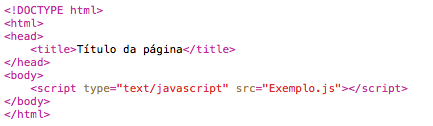
\includegraphics[scale=0.8]{./imagens/javascript_include.png}}
%	\caption[Exemplo de inclusão do código Javascript de um arquivo externo]
%	{Exemplo de inclusão do código Javascript de um arquivo externo. \textbf{Fonte:} Elaborado pelos autores.}
%	\label{fig:javascript_externo}
%\end{figure}

Para \citeonline{flanagan_javascript_definitive_guide}, as três tecnologias (HTML, CSS e Javascript) devem ser usadas em conjunto, uma vez que, cada uma delas possui seu papel específico, sendo eles: o HTML usado para especificar o conteúdo da página \textit{web}, o CSS para especificar como os componentes serão apresentados e o Javascript para especificar o comportamento da página.

Pelos motivos acima mencionados, somado ao fato de que o Javascript permite ao desenvolvedor criar páginas \textit{web} mais dinâmicas e flexíveis, atendendo perfeitamente os requisitos deste trabalho, essa tecnologia será utilizada para auxiliar na criação das páginas \textit{web} deste trabalho.

\subsection{Angular JS}

Segundo \citeonline{green_seshadri_angularjs}, o framework Angular JS foi criado para facilitar o desenvolvimento de aplicativos \textit{web}, pois através dele, é possível criar um aplicativo \textit{web} com poucas linhas.

Para o criador do Angular JS, Miško Hevery, o que o motivou a criar o Angular JS foi a necessidade de ter que reescrever determinados trechos de códigos em todos os outros projetos, o que para ele, tornou-se inviável. Portanto, Miško decidiu criar algo para facilitar o desenvolvimento de aplicativos \textit{web} de uma forma que ninguém havia pensado antes.

O Angular JS é um framework \textit{Model-View-Controller} - MVC\footnotemark[30] - escrito em Javascript. Ele é executado pelos navegadores de internet e ajuda os desenvolvedores a escreverem modernos aplicativos \textit{web} \cite{kozlowski_darwin_mastering_web_application_angular_js}.

\footnotetext[30]{MVC: \textit{Model-View-Controller} - \textit{Design pattern}.}

Devido às facilidades que o Angular JS nos traz, é que ele foi escolhido para ser utilizado, a fim de auxiliar no desenvolvimento, não apenas das páginas web e seus respectivos conteúdos, como também na lógica e comunicação com o \textit{Web Service} REST.


\chapter{QUADRO METODOLÓGICO}
\label{cap:quadroMetodologico}


\par Neste quadro metodológico serão apresentados os passos que se fizeram necessários para a realização desta pesquisa. Nele estão descritos desde a escolha do perfil da pesquisa até os procedimentos utilizados para o seu desenvolvimento. \citeonline{gil_metodos_e_tecnicas_de_pesquisa}, cita que a metodologia é um conjunto de procedimentos intelectuais e técnicos que trabalham para a realização do objetivo proposto.
\par Posterior ao estudo do levantamento teórico e técnico, foram definidos os procedimentos para a construção deste trabalho, iniciando pela escolha do tipo de pesquisa, demonstrada na seção a seguir.


%Será apresentado neste capítulo a metodologia de pesquisa a ser utilizada para a realização deste projeto e os passos necessários até a sua conclusão.

\section{Tipo de pesquisa}

\par Para \citeonline[p. 31]{padua_metodologia_pesquisa}, pesquisa é:

\begin{citacao}
	Toda atividade voltada para a solução de problemas; como atividade de busca, indagação, investigação, inquirição da realidade, e a atividade que visa nos permitir, no âmbito da ciência, elaborar um  conhecimento, ou um conjunto de conhecimentos, que nos auxilie na compreensão desta realidade e nos oriente em nossas ações.
\end{citacao}

% Comentário, pois estava repetindo demais o fato de utilizar  apesquisa aplicada no desenvolvimento do trabalho. 
%\par O tipo de pesquisa aplicada foi escolhido para o desenvolvimento da pesquisa, pois conforme \citeonline[p. 32]{cooper_schindler_metodos_pesquisa_administracao}, ela ``tem uma ênfase prática na solução de problemas, embora a solução de problemas nem sempre seja gerada por uma circunstância negativa.''

\par De forma objetiva, a pesquisa é o meio utilizado para buscar respostas aos mais diversos tipos de indagações, tendo por base procedimentos racionais e sistemáticos. A pesquisa é realizada quando se tem um problema e não se têm informações suficientes para solucioná-lo. Por meio desta sessão, tem-se como objetivo explicar o tipo de pesquisa que norteou o desenvolvimento deste trabalho, justificando também como ele se enquadra no tipo escolhido.

\par Pesquisar é um trabalho que envolve planejamento, para que ela seja satisfatória, o pesquisador precisa estar envolvido e  desenvolver habilidades técnicas que o levem a escolher o melhor caminho em busca da obtenção dos resultados.

\par Segundo \citeonline{fonseca_metodologia_da_pesquisa}, ter um método de pesquisa envolve o estudo dos fatores que compõem o contexto da pesquisa, tais como, a escolha do caminho e o planejamento do percurso. Essa escolha inicia-se com a definição do tipo de pesquisa utilizada. Para este trabalho, é utilizada a pesquisa aplicada, que é aquela cujo o pesquisador tem como objetivo aplicar os conhecimentos obtidos durante o período da pesquisa, em um projeto real, a fim de conhecer os seus resultados. \citeonline{gil_como_elaborar_projeto_de_pesquisa} afirma que este tipo de pesquisa dirige-se à solução de problemas específicos, de interesses locais.

%\par Conforme \citeonline[p. 32]{cooper_schindler_metodos_pesquisa_administracao}, a pesquisa aplicada tem uma ênfase prática na solução de problemas. 
\par Nesta pesquisa foram estudados os conceitos de banco de dados orientado à grafos e a sua aplicabilidade, desenvolvendo, por meio dos conhecimentos obtidos pela pesquisa, uma solução prática, disponibilizada por meio de um sistema \textit{web}, que auxilia na busca por mão de obra temporária, que não caracterize vínculo empregatício.

\par Seguindo o enquadramento desta pesquisa, ela deve ser aplicada a um contexto específico, conforme será abordado a seguir. 



%\par Seguindo esta ideia, este tipo de pesquisa será utilizado no desenvolvimento deste projeto, pois, o objetivo é gerar uma solução para o problema de localização de mão de obra, por meio de um sistema \textit{web}. Este projeto adequa-se perfeitamente ao tipo de pesquisa aplicada, uma vez que o mesmo busca analisar e gerar uma possível solução para o problema em destaque.

%Parágrafo utilizado no pré-projeto. Foi corrigido por Edilson no dia 02/04/15 e criado o parágrafo acima
%\par Este tipo de pesquisa será utilizada no desenvolvimento deste projeto, pois a mesma busca analisar o problema e gerar uma solução para o mesmo através de um aplicativo ou serviço.  Neste caso, será o desenvolvimento de um sistema \textit{web} que auxilia na busca por profissionais temporários.


\section{Contexto de pesquisa}
\par O trabalho informal é um elemento estrutural da economia no Brasil e nos países em desenvolvimento. Ele faz parte do cenário atual, crescente a cada dia, e contribui ativamente com a geração de renda. É considerado como um desdobramento do excesso de mão de obra, definido a partir de pessoas que criam sua própria forma de trabalho como estratégia de sobrevivência ou como forma alternativa de recolocação no mercado de trabalho. O fortalecimento deste tipo de trabalho ocorre a partir da construção de redes, formadas por parentes e amigos, criando laços de confiança que são fundamentais para o desempenho da atividade. No entanto, há uma grande dificuldade em se encontrar estes profissionais, uma vez que não há um lugar centralizado para divulgar o seu perfil profissional.

\par O desenvolvimento deste trabalhos se propôs atuar sob essa limitação. Uma pesquisa informal, realizada no sul de Minas Gerais, com pessoas de diferentes perfis sociais, constatou que uma aplicação, capaz de centralizar a busca por estes profissionais, seria muito bem aceita. A partir deste resultado, validou-se a ideia de construir um ambiente \textit{web} onde o trabalhador informal tem o espaço para centralizar suas habilidades e manter um perfil visível aos possíveis contratantes. Qualquer prestador de serviço informal pode ter acesso a este ambiente, desde que possua um dispositivo eletrônico capaz de se conectar a internet. 

\par O ambiente desenvolvido também visa facilitar ao contratante, a busca por estes profissionais, uma vez que não é fácil localizá-los por meio dos mecanismos de busca tradicionais. Desta forma existe um benefício mutuo, onde contratados e contratantes se despõem da praticidade.

\par Enfim, o contexto ao qual esta pesquisa se destina busca ser bem abrangente, com o intuito de contribuir de forma relevante, proporcionando uma boa experiência aos envolvidos.
 
%Exemplo de contexto que a Joelma deu na sala de aula. Usar como exemplo
%\par Este sistema volta-se para implantação e execução em todas as empresas de pequeno porte do ramo varejista no sul de minas gerais que tenha apresentado a necessidade de um controle mais rigoroso da sua entrada e saída de mercadorias

%Segundo a Joelma e o Márcio este seria o contexto da pesquisa: As pessoas que buscam mão de obra para determinados tipos de trabalho (contratantes) e as pessoas que disponibilizam tais mãos de obra (contratados ou prestadores de serviços).

%Antigo Contexto que a Joelma disse que estava muito geral na correção do pré-projeto
%\par Esta pesquisa terá como foco todas as pessoas que necessitam de mão de obra temporária para realizar tarefas domésticas e rotineiras, além daquelas que não ocorrem com tanta intensidade. Uma vez que o sistema será desenvolvido em uma plataforma \textit{web}, todas as pessoas terão fácil acesso ao serviço, sendo necessário apenas possuir uma comunicação com a internet.

%\par Esta pesquisa terá como foco todas as pessoas da região do sul de Minas Gerais, que necessitam de determinados tipos de mão de obra (contratantes), bem como para aqueles que necessitam de um espaço para divulgar esta oferta (contratados ou prestadores de serviços). Tomando por base que encontrar este tipo de profissional tem se tornado uma tarefa cada vez mais complicada, que acaba gerando transtornos na vida da população, pois, em muitos casos, a falta de opções leva a contratações equivocadas e infelizes.

%\par Como o sistema será desenvolvido em uma plataforma \textit{web}, todas as pessoas neste contexto terão fácil acesso ao serviço, permitindo a disseminação desta ferramenta, sendo necessário apenas possuir uma comunicação com a internet.


%\section{Participantes}

\par Participaram desta pesquisa dois acadêmicos e um professor orientador, sendo eles Andressa Faria, Edilson Justiniano e Márcio Emílio.
\par Andressa de Faria Giordano, acadêmica do 7º período do curso de bacharelado em Sistemas de Informação pela Universidade do Vale do Sapucaí - UNIVAS - com formação técnica e profissionalizante pelo Instituto Nacional de Pesquisa Tecnologica e Computacional - INPETTECC. Sua participação, neste projeto, será o levantamento dos requisitos e a elaboração de todos os diagramas descritos nas fases do ICONIX, a modelagem do banco de dados, a implantação da lógica de negócios, comunicação entre os módulos, acesso aos dados pelo sistema e a documentação do trabalho.

\par  Edilson Justiniano, acadêmico do 7º período do curso de bacharelado em Sistemas de Informação pela Universidade do Vale do Sapucaí - UNIVAS - com formação técnica e profissionalizante pelo Instituto Nacional de Pesquisa Tecnologica e Computacional - INPETTECC. Sua participação, neste projeto, será o levantamento dos requisitos e a elaboração de todos os diagramas descritos nas fases do ICONIX, a modelagem do banco de dados, a implantação da lógica de negócios, comunicação entre os módulos, acesso aos dados pelo sistema e a documentação do trabalho.

\par Márcio Emílio Cruz Vono de Azevedo,professor orientador, engenheiro elétrico em modalidade eletrônica pelo Instituto Nacional de Telecomunicações - INATEL - e mestre em Ciência da Computação pela Universidade Federal de Itajubá - UNIFEI. Professor do INATEL e da Universidade do Vale do Sapucaí - UNIVAS - na área de engenharia de \textit{software} e especialista em sistemas do Inatel.


\par A elaboração do texto escrito será realizado com base nas ações que serão desenvolvidas pelos participantes e serão feitas em conjunto.


\section{Instrumentos}

\par Os instrumentos de pesquisa são as ferramentas usadas para a coleta de dados. Como afirma \citeonline[p. 117]{marconi_lakatos_metodologia_trabalho_cientifico}, eles abrangem “desde os tópicos de entrevista, passando pelo questionamento e formulário, até os testes ou escala de medida de opiniões e atitudes”. Eles são de suma importância para o desenvolvimento de um projeto, pois visam a levantar o máximo de informações possíveis para nortear as tomadas de decisões. Para a realização desta pesquisa foram utilizados questionários e análise documental.

\par Segundo \citeonline{gil_como_elaborar_projeto_de_pesquisa}, o questionário é um dos procedimentos mais utilizados para obter informações, pois é uma técnica de custo razoável, apresenta as mesmas questões para todas as pessoas, garante o anonimato e pode conter as questões para atender a finalidades específicas de uma pesquisa. Se aplicada criteriosamente, essa técnica apresenta elevada confiabilidade. Os questionários podem ser desenvolvidos para medir opiniões, comportamento, entre outras questões, também pode ser aplicada individualmente ou em grupos.

\par Para este trabalho, foi desenvolvido um questionário informal, aplicado de forma individual, disponibilizado no ambiente virtual, o qual foi respondido com o intuito de analisar se a pesquisa aqui pretendida seria bem aceita por pessoas de diferentes perfis sociais. %A seguir são discriminados os resultados obtidos.

%Aqui colocar o resultado da análise do questionário

\par A análise documental consiste em identificar, verificar e apreciar os documentos, atendendo a uma finalidade específica, que visa extrair uma informação objetiva da fonte. Para este trabalho foi utilizada a análise documental como material de apoio, que norteou tanto o desenvolvimento teórico quanto o prático.

\par Feita a escolha dos instrumentos, foram definidos os procedimentos necessários para que a pesquisa fosse realizada. Estes procedimentos serão descritos na próxima seção.




%\subsection{Questionários}

\par Para \citeonline{silva_menezes_metodologia_pesquisa_elaboracao_dissertacao}, questionário é:

\begin{citacao}
	Uma série ordenada de perguntas que devem ser respondidas por escrito pelo informante. O questionário deve ser objetivo, limitado em extensão e estar acompanhado de instruções As instruções devem esclarecer o propósito de sua aplicação, ressaltar a importância da colaboração do informante e facilitar o preenchimento.
\end{citacao}

%\par Qual o objetivo de aplicar o questionário? Serão aplicados os questionários para a empresa tal, a fim de levantar o grau de satisfação dos funcionários com o sistema.

%\par Quantos ou quantas e para quem?

\par Serão disponibilizados questionários \textit{on-line} a fim de avaliar o interesse da população por um sistema que ofereça o serviço de localização de mão de obra temporária. Para desenvolver tal \textit{software}, uma bateria de testes será feita visando oferecer a melhor interação entre o usuário e o software, levando em conta sua aplicabilidade, desempenho e facilidade de utilização.

%\par A observação será feita através de formulários de pesquisa que avaliarão o interesse dos usuários pelo sistema que ofereça o serviço de localização de mão de obra temporária. Os testes serão feitos visando oferecer a melhor interação entre o usuário e o software, levando em conta sua aplicabilidade, desempenho e facilidade de utilização.


%Reunião não é aplicado ao nosso trabalho pq reunião não é um instrumento de pesquisa
%\section{Reuniões}

%\par Serão realizados encontros presenciais e também virtuais com os acadêmicos e com o professor orientador, para o levantamento dos requisitos, da aplicabilidade do software, dos modelos de engenharia de software e codificação do sistema, como também questões teóricas que estejam relacionadas com as melhores práticas para se obter um software aplicável e ágil.


%\subsection{Análise documental}

\par Para auxiliar no desenvolvimento deste projeto serão utilizados documentos como: manuais, tutoriais, livros, trabalhos e artigos acadêmicos, além de pesquisa web. Estes serão utilizados para o embasamento teórico que consiste no levantamento de requisitos e tecnologias a serem abordadas, e também para o desenvolvimento prático servindo como apoio e referencial para futuras consultas.


\section{Procedimentos}

\par Para que esta pesquisa fosse levada a cabo, tornou-se necessário a implementação de algumas ações, as quais serão detalhadas.

\par O início da pesquisa deu-se através da escolha do tema, seguido pelo levantamento das tecnologias que seriam utilizadas. A princípio, foi definido um escopo contendo algumas tecnologias que foram ministradas no ambiente acadêmico, o que diminui a curva de aprendizado, no entanto, foi preciso agregar alguns conhecimentos novos, onde foi desprendido um tempo a mais para estudo e realização de pequenos testes. As tecnologias que foram empregadas no desenvolvimento deste trabalho são as seguintes: a linguagem de programação JAVA, o banco de dados orientado a grafos Neo4j, juntamente com a API Cypher, Tomcat, Primefaces e JSF, sendo que no decorrer do desenvolvimento prático, viu-se a necessidade de substituir as duas ultimas tecnologias citadas pelas linguagens HTML, CSS, Javascript e Angular JS. As tecnologias que acompanharam o desenvolvimento deste trabalho até a sua conclusão estão descritas no quadro teórico desta pesquisa.

\par Para garantir que as tecnologias selecionadas seriam a melhor escolha no desenvolvimento deste trabalho, foram realizados alguns testes por meio de aplicações simples. Os testes foram focados na avaliação do comportamento do banco de dados orientado a grafos aplicado ao contexto desta pesquisa, cujo objetivo foi desenvolver uma aplicação de busca de mão de obra baseada em uma rede de relacionamentos. Estes testes também foram realizados como fins didáticos, a fim de se familiarizar com as tecnologias utilizadas.

\par Para garantir a qualidade desta pesquisa, o ICONIX foi escolhido como a metodologia de desenvolvimento de \textit{software}, desempenhando um papel fundamental na organização do trabalho. Sua abordagem proveu uma sequencia de procedimentos, que foram seguidos conforme o necessário, levando a construção de uma aplicação estável. Como relatado no quadro teórico, foram seguidas as quatro fases definidas pelo ICONIX.

\par Na primeira fase, definida como análise de requisitos, foi realizado o levantamento das informações pertinentes ao desenvolvimento da aplicação. Este levantamento foi realizado por meio da observação do comportamento das pessoas ao realizar essa busca por mão de obra temporária. A partir dai, foram levantadas as principais características, que seriam indispensáveis para o desenvolvimento deste trabalho e criado o modelo de domínio inicial do projeto como demonstra a Figura 15, com base nas informações levantadas. Nesta fase também foram definidas todas as ações que o usuário poderia realizar no sistema, por meio dos casos de uso, conforme a Figura 16.

\newpage
\begin{figure}[h!]
	\centerline{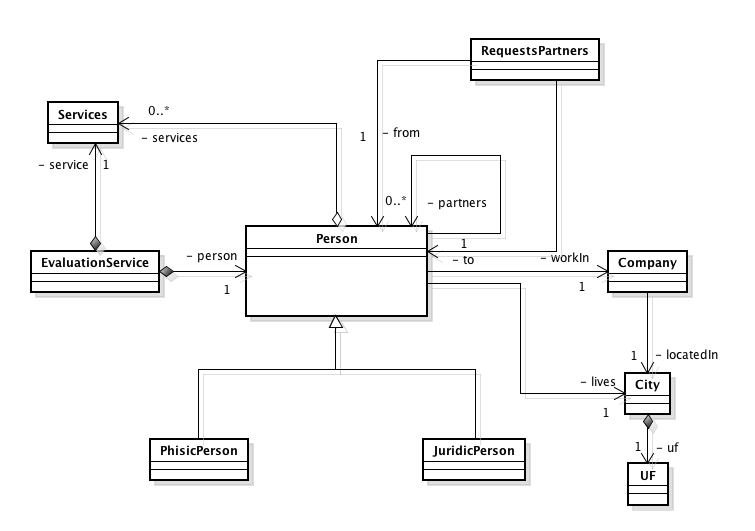
\includegraphics[scale=0.45]{./imagens/modelo-dominio-inicial.png}}
	\caption[Modelo de domínio inicial]
	{Modelo de domínio inicial. \textbf{Fonte:} Elaborado pelos autores.}
	\label{fig:exemplo1}
\end{figure}

\begin{figure}[h!]
	\centerline{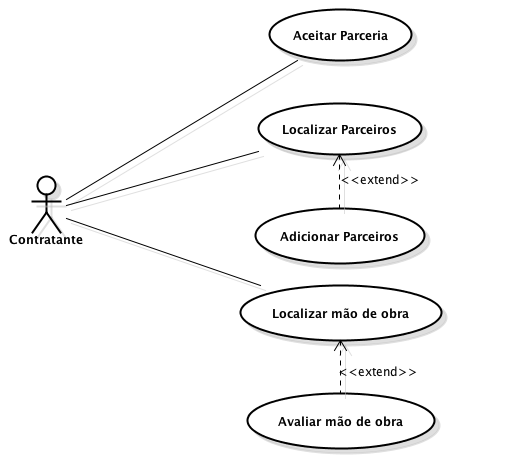
\includegraphics[scale=0.6]{./imagens/caso-de-uso.png}}
	\caption[Diagrama de caso de uso]
	{Diagrama de caso de uso. \textbf{Fonte:} Elaborado pelos autores.}
	\label{fig:exemplo1}
\end{figure}

\par Na segunda fase, análise e projeto preliminar, houve um refinamento dos requisitos levantados na fase anterior, definindo melhor as ações do usuário, por meio dos diagramas de casos de uso. Posterior a esta definição foram gerados os diagramas de robustez, de acordo com os casos de uso definidos, como demonstra a Figura 17. Paralelamente a modelagem desses diagramas, foi atualizado o modelo de domínio, acrescentando os atributos identificados, conforme a Figura 18. Com o modelo de domínio atualizado, foi feita a modelagem do banco de dados da aplicação como apresenta a Figura 19.

\begin{figure}[h!]
	\centerline{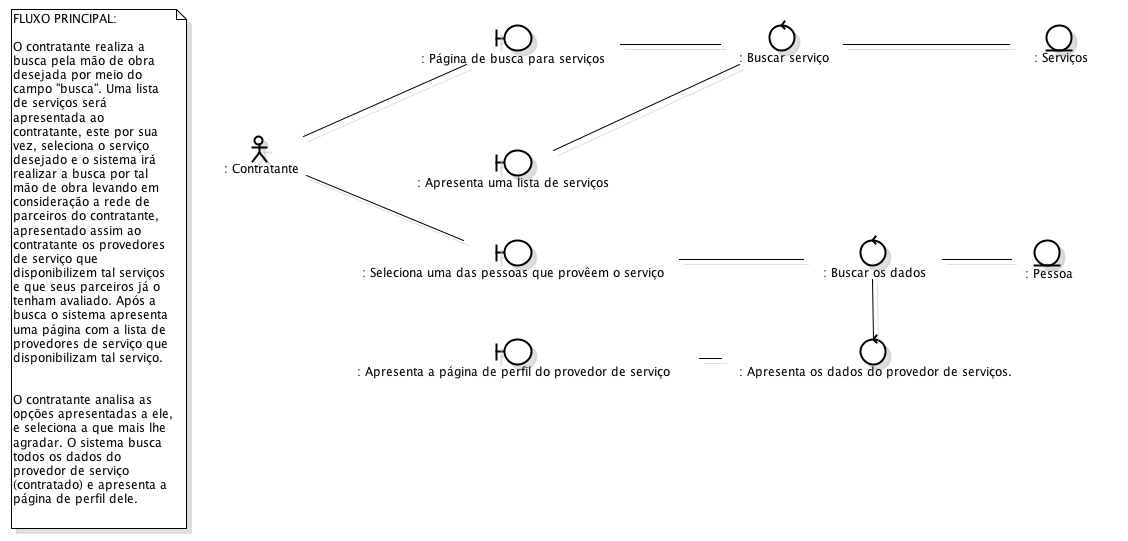
\includegraphics[scale=0.35]{./imagens/robustez.png}}
	\caption[Diagrama de robustez do caso de uso Localizar mão de obra]
	{Diagrama de robustez do caso de uso Localizar mão de obra. \textbf{Fonte:} Elaborado pelos autores.}
	\label{fig:exemplo1}
\end{figure}

\begin{figure}[h!]
	\centerline{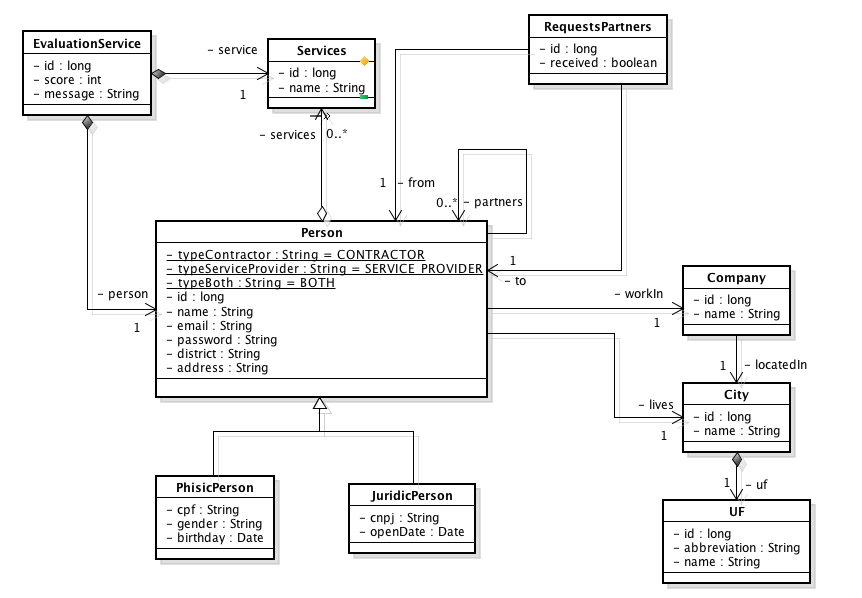
\includegraphics[scale=0.6]{./imagens/modelo-dominio-com-atributos.png}}
	\caption[Modelo de domínio atualizado]
	{Modelo de domínio atualizado. \textbf{Fonte:} Elaborado pelos autores.}
	\label{fig:exemplo1}
\end{figure} 

\begin{figure}[h!]
	\centerline{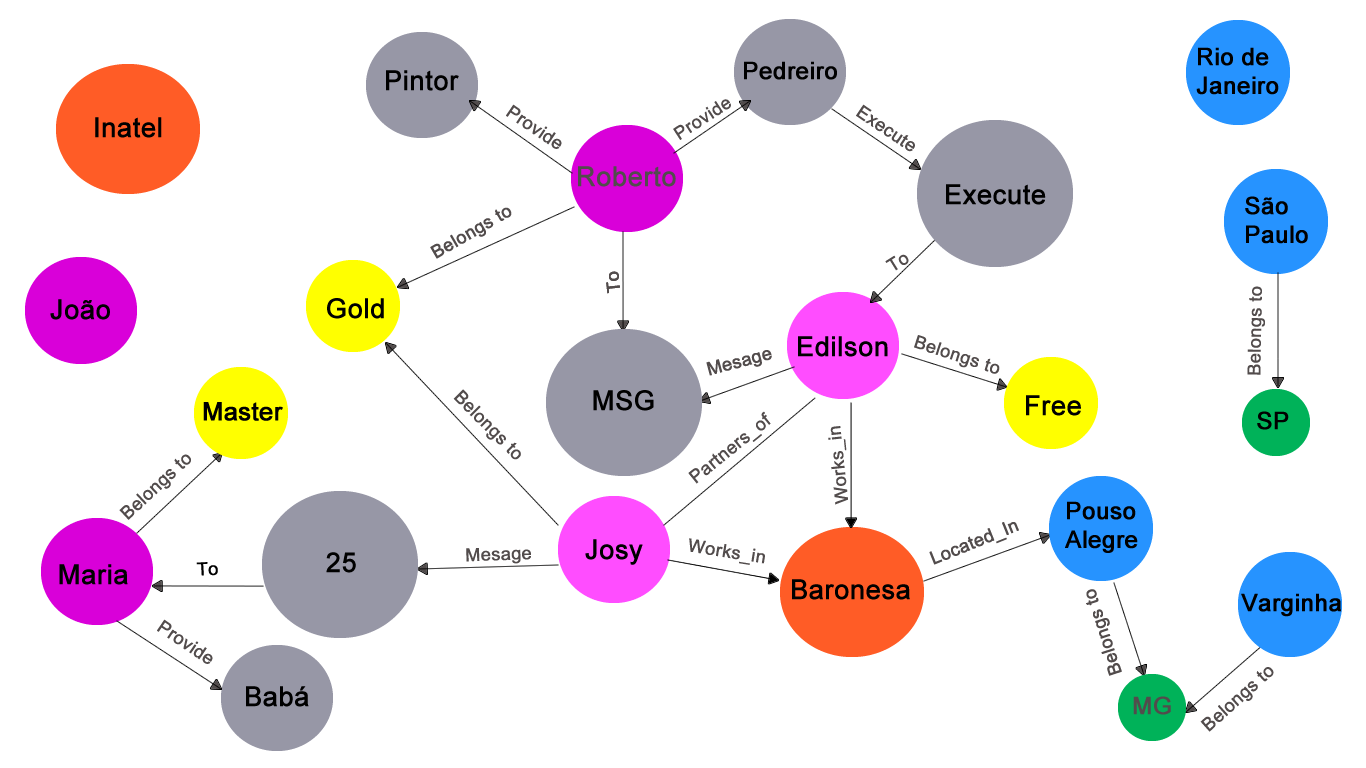
\includegraphics[scale=0.5]{./imagens/structure-all-nodes.png}}
	\caption[Modelo de dados da aplicação]
	{Modelo de dados da aplicação. \textbf{Fonte:} Elaborado pelos autores.}
	\label{fig:exemplo1}
\end{figure} 


\par Na terceira fase, definida como projeto detalhado, foram criados os diagramas de sequencia, tendo como base os casos de uso modelados na fase anterior. Esta fase tem como objetivo detalhar todo o funcionamento do \textit{software}, visando definir a melhor maneira de realizar sua implementação. A Figura 20 apresenta o diagrama de sequência do caso de uso localizar mão de obra.

\newpage
\begin{figure}[h!]
	\centerline{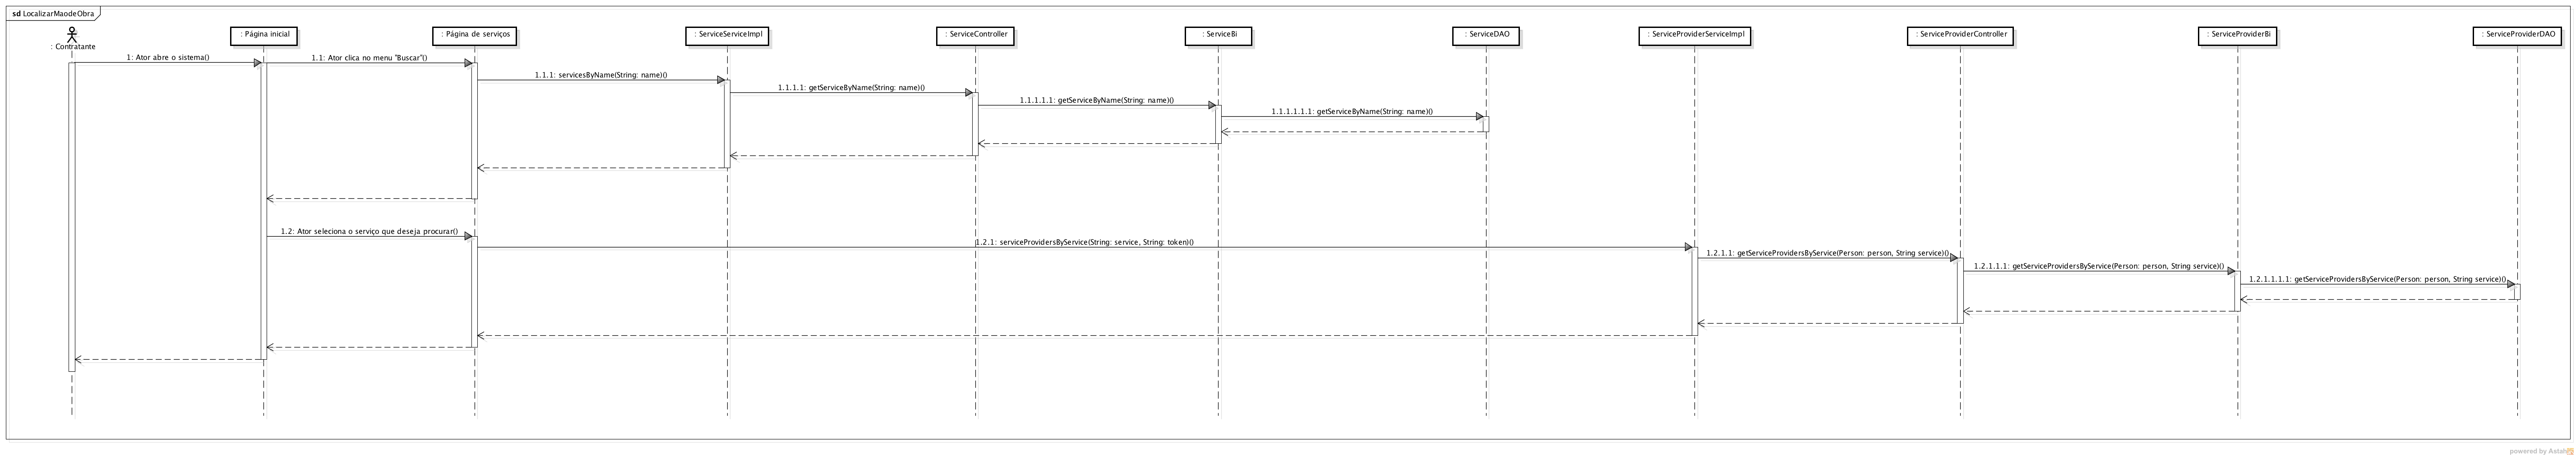
\includegraphics[angle=90,height=0.7\textheight,width=0.7\textwidth]{./imagens/sequence-localizar-mao-de-obra.png}}
	\caption[Diagrama de caso de uso]
	{Diagrama de caso de uso \textbf{Fonte:} Elaborado pelos autores.}
	\label{fig:exemplo1}
\end{figure}

\par Ainda na fase de projeto detalhado, após a modelagem dos diagramas de sequencia, as operações encontradas nestes diagramas foram adicionadas ao modelo de domínio, em conjunto com as novas classes identificadas, gerando assim, o digrama de classes.

imagem do diagrama de classes


\par Na quarta e última fase do ICONIX, denominada implementação, iniciou-se a preparação do ambiente de desenvolvimento, incluindo a instalação de \textit{softwares} adicionais, necessários para o desenvolvimento prático da aplicação.

\par Visto que o trabalho seria desenvolvido em equipe, foi necessário estabelecer uma ferramenta de controle de versão. Esta ferramente permitiu o gerenciamento de diferentes versões de arquivos, gerando um histórico contendo as modificações que foram realizadas no decorrer do processo de desenvolvimento. Este histórico permite o retorno de alguma revisão, caso haja necessidade. A ferramenta escolhida para realizar esse controle foi o GitHub, que já havia sido utilizado em alguns trabalhos do contexto acadêmico, evitando o desprendimento de tempo para estudo de uma nova ferramenta de apoio. O GitHub é uma ferramenta bem difundida e permite que os seus usuários colaborem com os projetos que estão armazenados em seus repositórios\footnotemark[31]. A Figura 21 demonstra a tela de serviços provida pelo GitHub.

\footnotetext[31]{Repositório: local cujo desenvolvedor utiliza para armazenar os documentos relacionados ao \textit{software}.}

\begin{figure}[h!]
	\centerline{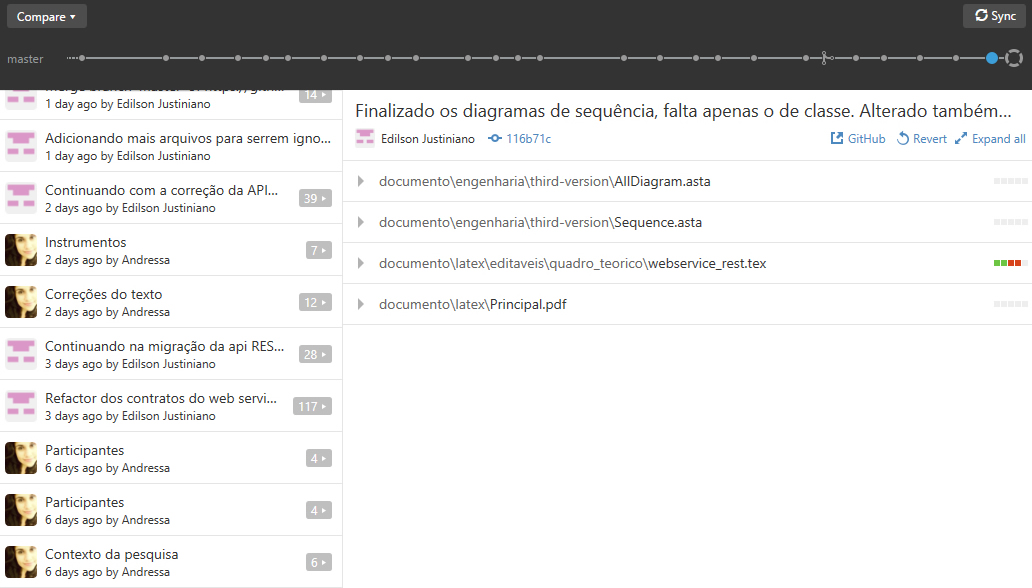
\includegraphics[scale=0.35]{./imagens/github.jpg}}
	\caption[Tela de serviços do GitHub ]
	{Tela de serviços do GitHub \textbf{Fonte:} Elaborado pelos autores.}
	\label{fig:exemplo1}
\end{figure}

\par Os passos de instalação detalhados do GitHub são descritos na sessão apêndices deste trabalho.

\par Como mencionado no quadro teórico, neste trabalho foi utilizada a linguagem Java, sendo assim necessário a utilização de uma IDE de apoio. A IDE escolhida foi o Eclipse, pois se trata de uma ferramenta \textit{open source}, bem difundida no mercado e que permite a escrita de um código mais legível, facilitando tarefas como \textit{debug} e configurações do projeto.

\par O Eclipse possui várias ferramentas, dentre elas, pode-se citar o editor de texto, utilizado não somente para a escrita de códigos em Java, e também a perspectiva de configuração para servidores \textit{web}, utilizada neste trabalho, conforme apresenta a Figura 22. Por meio desta perspectiva, foi configurada a aplicação \textit{container} Tomcat na versão 7.

\newpage
\begin{figure}[h!]
	\centerline{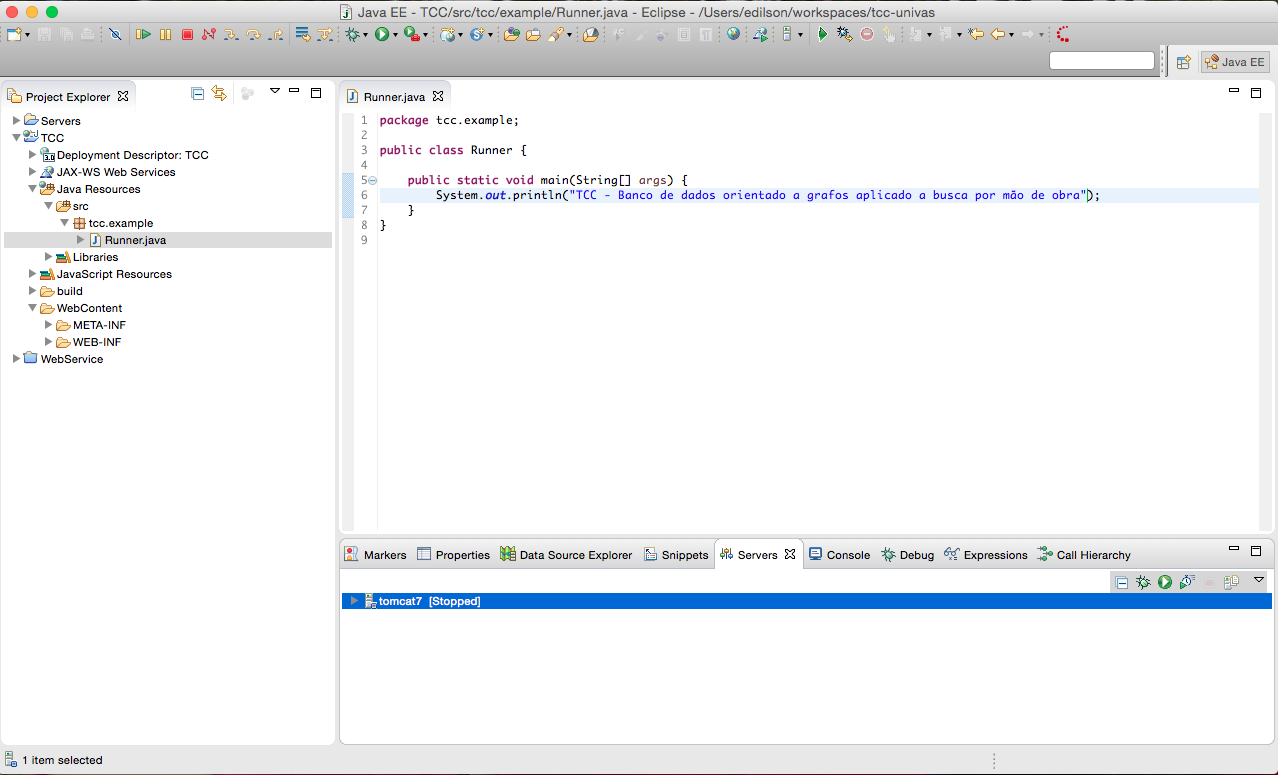
\includegraphics[scale=0.35]{./imagens/eclipse-editor-texto.png}}
	\caption[Ferramentas da IDE Eclipse]
	{Ferramentas da IDE Eclipse \textbf{Fonte:} Elaborado pelos autores.}
	\label{fig:exemplo1}
\end{figure}

\par O Tomcat desempenhou um papel fundamental na execução desta aplicação, pois serviu como hospedeiro para a aplicação Java desenvolvida neste trabalho. 

\par Os passos de instalação e configuração do Eclipse e do Tomcat são descritos na sessão apêndices deste trabalho.

\par Para a escrita do código relacionado ao HTML, CSS e Javascript, foi utilizado o mesmo editor de texto citado anteriormente.

\par O trabalho fez uso de um banco de dados orientado a grafos, o Neo4j. A escolha desse banco se deu pela sua simplicidade de instalação, configuração, facilidade de integração com a API \textit{Cypher} e por disponibilizar uma API REST para acesso aos seus dados, conforme descrito no quadro teórico deste trabalho. O Neo4j faz parte do enquadramento de softwares livres, seguindo o conceito \textit{open source}, o que permite ao desenvolvedor utilizá-lo da forma que melhor lhe convém. 


\par A seguir serão detalhados os passos para a instalação do banco de dados Neo4j.

\par Para realizar o \textit{download} do instalador do banco de dados Neo4j, deve-se acessar a seguinte url, por meio de um  navegador de internet: http://neo4j.com/download e selecionar a opção desejada. Neste trabalho como já descrito foi utilizada a versão \textit{Community}. A Figura 23 apresenta a página de download do Neo4j.

\newpage
\begin{figure}[h!]
	\centerline{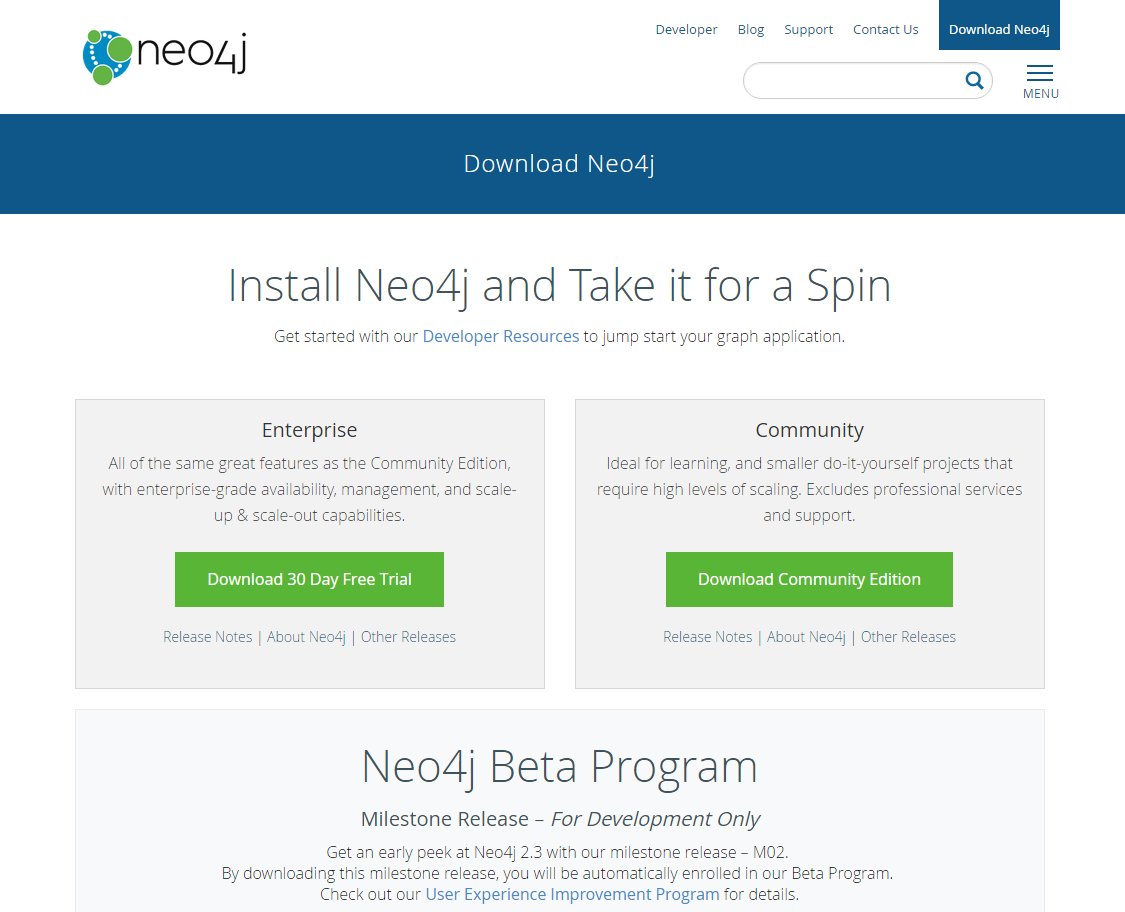
\includegraphics[scale=0.4]{./imagens/download-neo4j.png}}
	\caption[Página de download do Neo4j]
	{Página de download do Neo4j. \textbf{Fonte:} http://neo4j.com/download}
	\label{fig:exemplo1}
\end{figure}

\par Após concluído o \textit{download}, deve-se executar o arquivo. O processo de instalação se inicia e, a primeira tela apresentada ao usuário é a tela contendo uma mensagem de boas vindas, conforme demonstra a Figura 24. Nesta tela, deve-se clicar no botão \textit{Next} para prosseguir com o processo de instalação.

\begin{figure}[h!]
	\centerline{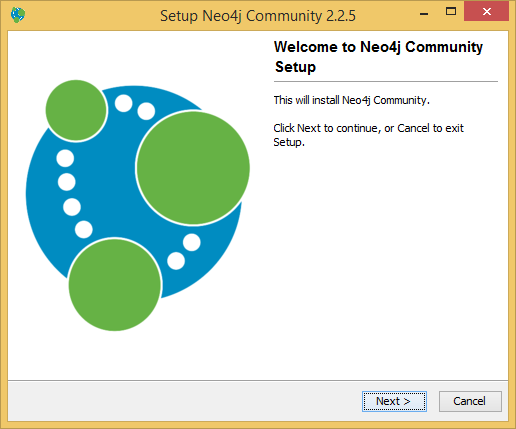
\includegraphics[scale=0.4]{./imagens/neo4j-install-step1.png}}
	\caption[Tela de boas vindas da instalação do Neo4j]
	{Tela de boas vindas da instalação do Neo4j. \textbf{Fonte:} Elaborado pelos autores.}
	\label{fig:exemplo1}
\end{figure}

\par A próxima tela apresentada ao usuário diz respeito ao contrato de uso do \textit{software}, como mostra a Figura 25. Após lê-lo, deve-se aceitar os termos do contrato e clicar no \textit{Next}.

\newpage
\begin{figure}[h!]
	\centerline{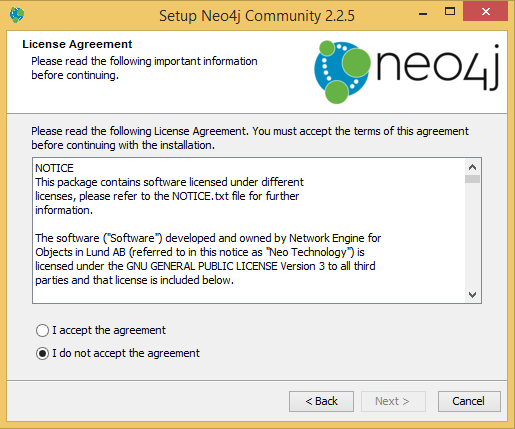
\includegraphics[scale=0.4]{./imagens/neo4j-install-step2.png}}
	\caption[Tela do contrato de uso do Neo4j]
	{Tela do contrato de uso do Neo4j. \textbf{Fonte:} Elaborado pelos autores.}
	\label{fig:exemplo1}
\end{figure}

\par Na próxima tela, conforme a Figura 26 demonstra, é definido o diretório de instalação do Neo4j. Por padrão este diretório é o mesmo das demais aplicações no Windows, podendo ser alterado conforme a necessidade. Após definir o diretório de instalação deve-se clicar no botão \textit{Next}.

\begin{figure}[h!]
	\centerline{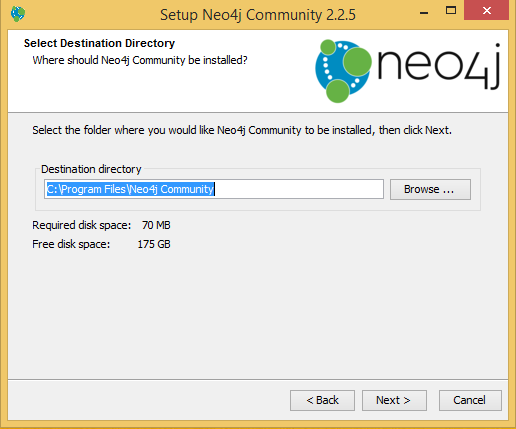
\includegraphics[scale=0.4]{./imagens/neo4j-install-step3.png}}
	\caption[Tela para definição do diretório de instalaão do Neo4j]
	{Tela para definição do diretório de instalaão do Neo4j. \textbf{Fonte:} Elaborado pelos autores.}
	\label{fig:exemplo1}
\end{figure}

\par Após as definições anteriores, uma tela é apresentada questionando ao usuário a respeito da criação de atalhos na área de trabalho, como é demonstrado na Figura 27. Após definir os atalhos do Neo4j, deve-se clicar no botão \textit{Next}.

\begin{figure}[h!]
	\centerline{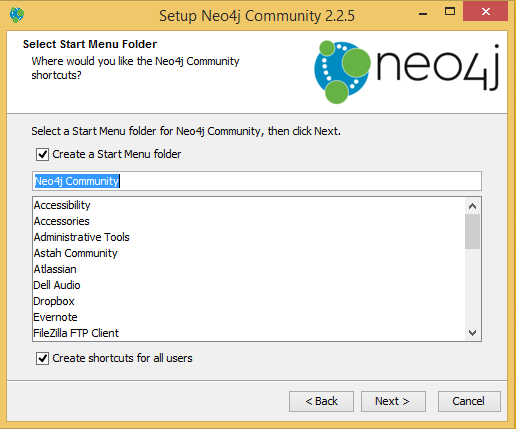
\includegraphics[scale=0.4]{./imagens/neo4j-install-step4.png}}
	\caption[Tela para criação de atalhos do Neo4j]
	{Tela para criação de atalhos do Neo4j. \textbf{Fonte:} Elaborado pelos autores.}
	\label{fig:exemplo1}
\end{figure}

\par Após realizar os procedimentos descritos para a instalação do Neo4j a tela final de instalação será apresentada, informando-o a respeito do resultado da instalação conforme demonstra a Figura 28. Clique no botão \textit{Finish} para finalizar o processo de instalação.
Após todos os passos realizados com sucesso, o Neo4j estará disponível.

\begin{figure}[h!]
	\centerline{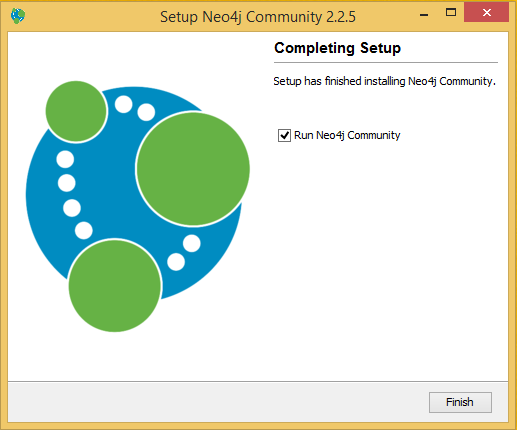
\includegraphics[scale=0.4]{./imagens/neo4j-install-step5.png}}
	\caption[Tela final de instalação do Neo4j]
	{Tela final de instalação do Neo4j. \textbf{Fonte:} Elaborado pelos autores.}
	\label{fig:exemplo1}
	
\end{figure}

\par A Figura 29 e 30 apresentam a tela inicial do banco de dados Neo4j e um exemplo de consulta realizada por meio da aplicação de gerencia da base de dados.

\begin{figure}[h!]
	\centerline{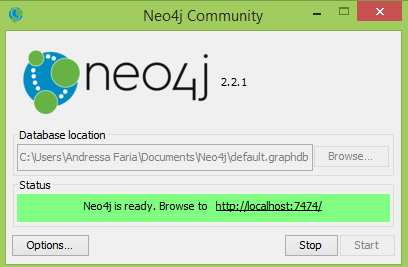
\includegraphics[scale=0.60]{./imagens/neo4j.jpg}}
	\caption[Tela de inicialização do Neo4j ]
	{Tela de inicialização do Neo4j \textbf{Fonte:} Elaborado pelos autores.}
	\label{fig:exemplo1}
\end{figure}

\begin{figure}[h!]
	\centerline{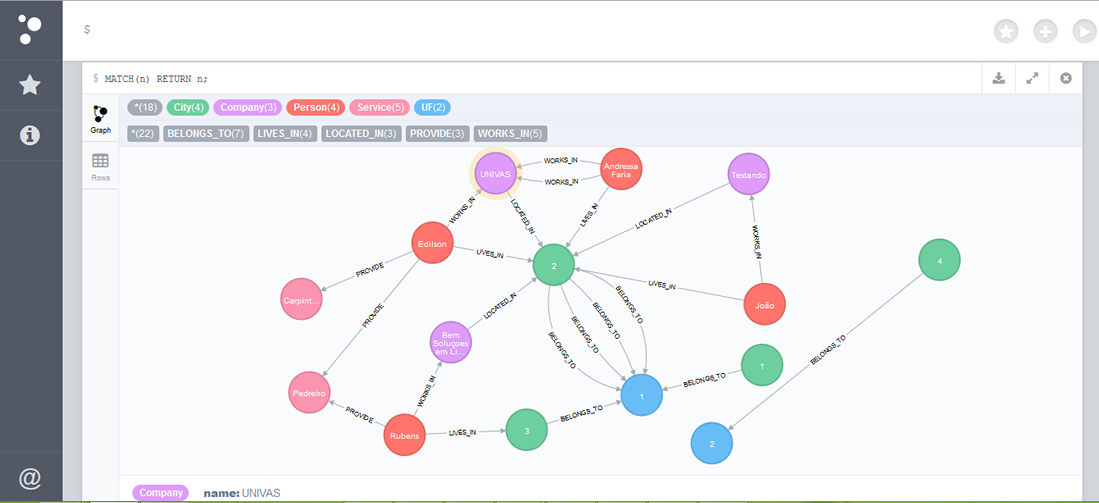
\includegraphics[scale=0.4]{./imagens/neo4j2.jpg}}
	\caption[Demonstração de uma consulta Cypher.]
	{Demonstração de uma consulta Cypher. \textbf{Fonte:} Elaborado pelos autores.}
	\label{fig:exemplo1}
\end{figure}
 
\newpage

\par Posterior a configuração do ambiente, iniciou-se o desenvolvimento propriamente dito. A princípio, utilizou-se as tecnologias Neo4j, sendo executado de forma \textit{embedded}, Primefaces e JSF. Porem não estava fluindo como o esperado, uma vez que o Neo4j utilizado desta maneira não permitia conectar ao sistema de gerenciamento da base de dados e abrir uma nova instancia de conexão simultânea, devido a limitações do próprio Neo4j, uma vez que um processo Java já ocupava tal conexão com o \textit{socket} do banco de dados.

\par Outro problema encontrado ao utilizar tais tecnologias foi que tanto a parte cliente (\textit{front end}) quanto a parte servidor (\textit{back end}) se encontravam totalmente acoplados em uma aplicação Java \textit{web}, portanto, a cada alteração realizada havia a necessidade de recompilar, construir e publicar a aplicação no servidor \textit{web}, impedindo que o desenvolvimento do \textit{software} fluísse, como era esperado. Por esses motivos decidiu-se mudar algumas das tecnologias utilizadas no \textit{front end} e, a maneira como o banco de dados era acessado até então. 

\par Posterior a esse incidente, passou-se a utilizar então as linguagens HTML 5, CSS 3, Java Script e Angular JS para auxiliar no desenvolvimento do \textit{front end}, ao invés de Primefaces e JSF. Para acesso ao banco de dados, lançou-se mão da forma \textit{embedded} e passou-se a utilizar a API REST disponibilizada pelo próprio banco. Tais decisões nos permitiram desacoplar o sistema e manter o \textit{front end} e o \textit{back end} independentes, evitando assim, que o mesmo problema voltasse a ocorrer.

\par Como a forma de conexão ao banco de dados foi alterada, houve-se a necessidade de reescrever a classe responsável por realizar esta conexão. Ao utilizar esta nova abordagem de conexão ao banco de dados, foi necessário informar o \textit{hostname} e a porta IP cujo banco está instalado e o diretório onde os dados estão localizados internamente no Neo4j. Neste trabalho foi utilizado o diretório padrão (/db/data). Após realizada esta configuração, foi necessário acrescentar o parâmetro ''/cypher'' à criação da instância de conexão, a fim de utilizar a API \textit{Cypher} em conjunto com esta nova abordagem, conforme apresenta a Figura 31.

\begin{figure}[h!]
	\centerline{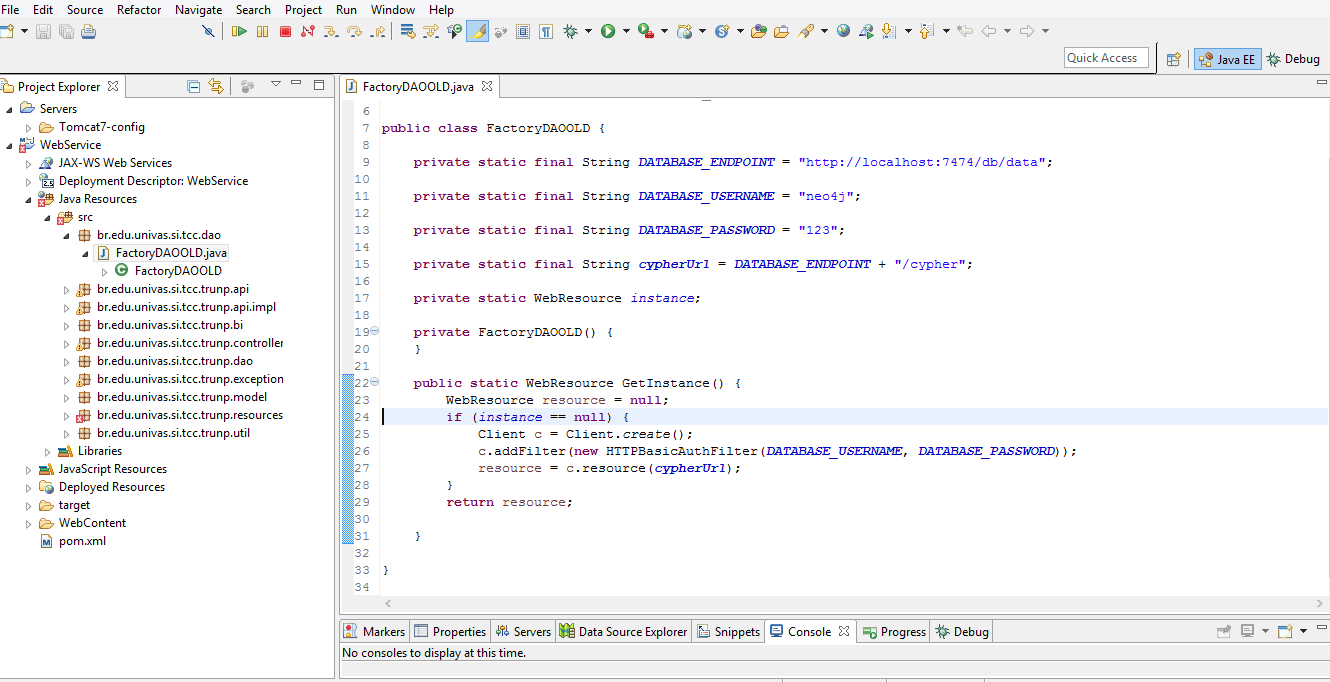
\includegraphics[scale=0.35]{./imagens/conexao-banco.jpg}}
	\caption[Código de comunicação com o banco]
	{Código de comunicação com o banco \textbf{Fonte:} Elaborado pelos autores.}
	\label{fig:exemplo1}
\end{figure}

\par Após realizar a mudança de tecnologias, foi necessário realizar alguns testes para compreender o funcionamento do \textit{web service} REST e paralelamente foi feito o levantamento de materiais de referência do \textit{framework} Angular JS. Foi preciso realizar testes para validar a conexão com o banco de dados Neo4j via API REST, fornecida por ele. Também foram realizados testes para envio de requisições e recebimento de respostas do \textit{web service} REST, utilizando o Angular JS. Para validar a conexão ao banco de dados via API REST foi necessário desenvolver algumas consultas em \textit{cypher} como apresenta a Figura 32.

\newpage
\begin{figure}[h!]
	\centerline{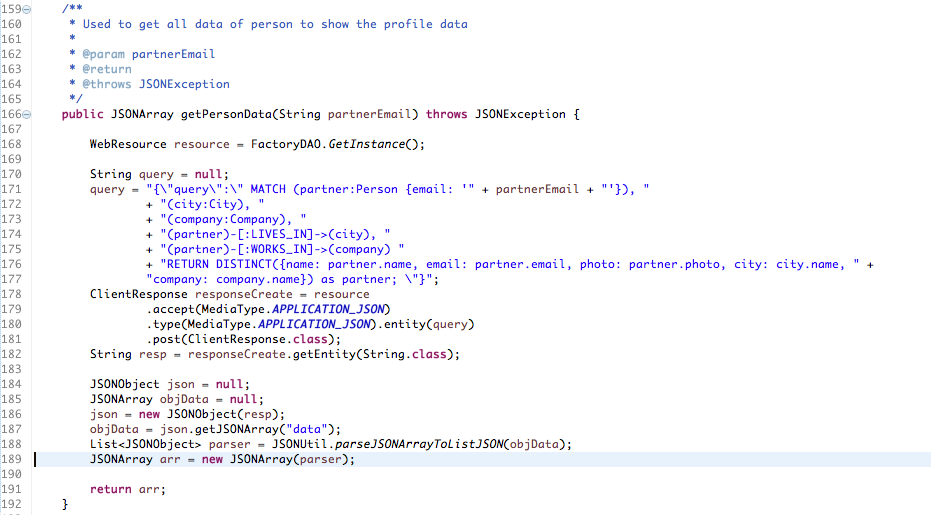
\includegraphics[scale=0.45]{./imagens/query-cypher.png}}
	\caption[Exemplo de consulta usando a API \textit{cypher}]
	{Exemplo de consulta usando a API \textit{cypher}. \textbf{Fonte:} Elaborado pelos autores.}
	\label{fig:exemplo1}
\end{figure}

\par Ao realizar estes testes foi constatado que seria necessário desenvolver uma maneira de converter os resultados das buscas realizadas no banco de dados Neo4j que, por padrão não retorna os resultados no formato JSON comum para um JSON válido, portanto, houve-se a preocupação em tratar estas respostas, a fim de retornar um JSON válido ao usuário que futuramente viria a utilizar a API REST fornecida por este \textit{software}. É possível visualizar este tratamento na Figura 32. 
 
\par A partir deste ponto, a aplicação estava totalmente desacoplada, sendo necessário realizar uma configuração, a fim de permitir que as requisições enviadas pelo \textit{front end} fossem aceitas pelo \textit{back end}, localizado em outro domínio.

\par Devido a mudança de tecnologias já comentadas, houve-se a necessidade de atualizar os diagramas de sequencia e de classe, inserindo os contratos de serviços do \textit{web service} REST. Com a definição deste contrato, deu-se início ao desenvolvimento dos casos de uso, identificados na primeira fase do ICONIX. 

\par Posterior a realização dos testes e da escolha definitiva da arquitetura que seria utilizada, iniciou-se a implementação dos casos de uso. O primeiro a ser implementado foi o caso de uso de criação de conta. Para este caso de uso, teve-se o cuidado de criar um mecanismo de criptografia de dados sigilosos, como usuário e senha, visando garantir a segurança da aplicação. Estas informações criptografadas são enviadas a cada requisição e validadas pelo \textit{web service}, sendo atualizadas caso sejam válidas, tornado mais complexo a quebra desta criptografia. Este mecanismo foi desenvolvido com base no sistema de \textit{login} via \textit{token}. Segundo o embasamento usado na criação de contas, deu-se início ao desenvolvimento do sistema de \textit{login} e \textit{logoff}, que também utilizam o conceito de criptografia via \textit{token}. 

Imagem tela de login

\par Com o funcionamento do sistema de login, passou-se a desenvolver a página inicial da aplicação. Esta página contém as informações que são restritas ao usuário cadastrado, podendo ser eles: contratantes, provedores de serviço ou ambos. O sistema apresenta uma página inicial diferente para cada tipo de conta, contendo apenas as informações que são liberadas de acordo com o acesso do usuário, sendo essas informações relatórios, últimas atualizações na rede de parceiros, avaliações de serviços e prováveis parceiros.

imagem das 3 contas.

\par O caso de uso localizar parceiros foi desenvolvido após a conclusão do caso de uso criar conta. A lógica deste caso de uso consiste em localizar os possíveis parceiros, com base na rede de parceria do contrante.

imagem localizar parceiro



\par Ainda relacionado ao tipo de conta contratante ou ambos, foi implementado o caso de uso adicionar parceiro, que permite ao usuário convidar um possível parceiro para fazer parte da sua rede. Após a implementação da lógica para adicionar um novo parceiro, houve-se a necessidade de implementar o serviço de requisições de parcerias, uma vez que não bastava apenas um contratante convidar outro para se tornarem parceiros, mas sim que o contratante convidado aceitasse sua solicitação de parceria, para assim se tornarem parceiros. Visando disponibilizar estas solicitações de forma agradável ao usuário, foi desenvolvida uma funcionalidade para que o usuário pudesse aceitar ou rejeitar a solicitação enviada à ele.

imagem aqui :D

\par Após realizada a implementação do caso de uso adicionar parceiro, houve-se a necessidade de desenvolver a busca por todos os usuário que possuiam o tipo de conta contratante ou ambos e que possuiam um relacionamento de parceria com o usuário autenticado no sistema, além da funcionalidade de localizar novos parceiros, baseando-se na localização da empresa na qual o usuário trabalha e na cidade onde ele vive, sempre ordenando os resultados por meio da quantidade de parceiros em comum. 

\par O caso de uso gerenciar serviços foi implementado em sequência, abrangendo as principais funcionalidaes de gerenciamento: cadastrar e adicionar um novo serviço ao usuário, cujo tipo de conta é provedor de serviços, listar os serviços atribuídos a ele, e remover serviços quando necessário. Visando melhorar a usabilidade, foi implementado um mecanismo de busca, que permitiu filtrar os resultados por meio de um campo que possui a função  auto completar, evitando assim, possíveis erros e diminuindo o tempo gasto pelo usuário para adicionar o serviço. A função realiza a busca em uma lista de serviços anteriormente cadastrados, no entanto, caso não haja o serviço solicitado, o usuário tem a liberdade de cadastrá-lo e atribuí-lo a si mesmo.

\par A partir deste ponto, foi possível iniciar o desenvolvimento do caso de uso localizar mão de obra, uma vez que, este caso de uso dependia diretamente das implementações das funcionalidades adicionar parceiros para os usuários contratantes e adicionar serviços aos provedores de serviço. Para facilitar a localização e deixar o \textit{software} mais usual, esta busca se basea inicialmente no serviço buscado pelo usuário, sendo posteriormente modificada para também levar em consideração a funcionalidade avaliar serviço que foi implementada paralelamente. A avaliação de serviço permite ao contratante dar uma nota ao serviço que foi prestado a ele. Com estas informações foi possível desenvolver uma busca que levaria em consideração, além destas informações, a rede de parceiros do usuário contratante, a fim de lhe apresentar as melhores opções possíveis.

\par A fim de abranger a busca e possibilitar que novos prestadores de serviços sejam avaliados pelos contratantes, a consulta que antes apresentava apenas provedores de serviços que possuiam avaliações, sendo elas, positivas ou negativas, foi ampliada, possibilitando que profissionais não avaliados também entrassem na lista de prováveis provedores de serviços.

\par Para auxiliar na tomada de decisão do usuário contratante, foi implementada uma funcionalidade que realiza o cálculo da média de um determinado serviço prestado por um usuário provedor de serviço, tomando como base as avaliações da rede de parceiros do usuário autenticado, da empresa onde ele trabalha e da cidade onde vive, oferecendo assim uma forma simples de ter acesso a qualidade do serviço prestado. *******************************

\par Após realizada todas as implementações já descritas, houve-se a preocupação de desenvolver uma interface, que além de amigável fosse prática ao usuário, desta forma, foi disponibilizada algumas informações relevantes, que auxiliam o usuário a compreender o que está ocorrendo em sua rede de parceria. Como exemplo é possível citar a lista de parceiros em comum entre o usuário autenticado no sistema e um determinado contratante por meio da página de perfil dele.

\par A fim de agregar mais funcionalidades para o usuário provedor de serviços, foi criado na página inicial do \textit{software} uma funcionalidade que visa apresentar algumas dicas interessantes que contribui com a sua imagem perante ao \textit{software}, levando-o assim a obter uma quantidade maior de oportunidades de trabalho.

\par Para finalizar o desenvolvimento foram desenvolvidos gráficos que apresentam ao usuário informações a respeito da qualidade do serviço prestado pelo provedor de serviços, comparando-os com os demais prestadores.

\par Realizado todos os procedimentos apresentados nesta sessão foi possível obter como resultado final a conclusão deste trabalho.

%\newpage
\section{Cronograma}

\par Será exibido aqui uma tabela contendo o cronograma a ser seguido por este projeto, desde a sua definição até a sua conclusão.

\begin{table}[htbp]
	\scriptsize
	\centering
	\begin{tabular}{|p{60mm}|p{3mm}|p{3mm}|p{3mm}|p{3mm}|p{3mm}|p{3mm}|p{3mm}|p{3mm}|p{3mm}|p{3mm}|p{3mm}|p{3mm}|}%Largura das colunas
		\hline\vspace{.99cm} %adicionando o espaçamento para que o nome dos meses caibam verticalmente
		\textbf{Ação} / \textbf{Mês} & 
		\parbox[t]{2mm}{\multirow{3}{*}{\rotatebox[origin=c]{90}{Janeiro}}} & \parbox[t]{2mm}{\multirow{3}{*}{\rotatebox[origin=c]{90}{Fevereiro}}} & 
		\parbox[t]{2mm}{\multirow{3}{*}{\rotatebox[origin=c]{90}{Março}}} & 
		\parbox[t]{2mm}{\multirow{3}{*}{\rotatebox[origin=c]{90}{Abril}}} &
		\parbox[t]{2mm}{\multirow{3}{*}{\rotatebox[origin=c]{90}{Maio}}} &
		\parbox[t]{2mm}{\multirow{3}{*}{\rotatebox[origin=c]{90}{Junho}}} &
		\parbox[t]{2mm}{\multirow{3}{*}{\rotatebox[origin=c]{90}{Julho}}} &
		\parbox[t]{2mm}{\multirow{3}{*}{\rotatebox[origin=c]{90}{Agosto}}} &
		\parbox[t]{2mm}{\multirow{3}{*}{\rotatebox[origin=c]{90}{Setembro}}} &
		\parbox[t]{2mm}{\multirow{3}{*}{\rotatebox[origin=c]{90}{Outubro}}} &
		\parbox[t]{2mm}{\multirow{3}{*}{\rotatebox[origin=c]{90}{Novembro}}} &
		\parbox[t]{2mm}{\multirow{3}{*}{\rotatebox[origin=c]{90}{Dezembro}}} \\
		\hline 
		Definição do Pré projeto & \cellcolor[HTML]{000000} &  &  &  &  &  &  &  &  &  &  & \\ \hline %1ª linha da tabela
		
		Aprovação do Pré projeto &  & \cellcolor[HTML]{000000} &  &  &  &  &  &  &  &  &  & \\ \hline %2ª linha
		
		Levantamento bibliográfico & \cellcolor[HTML]{000000} & \cellcolor[HTML]{000000} & \cellcolor[HTML]{000000} &  &  &  &  &  &  &  &  & \\ \hline %3ª linha
		
		Primeira entrega do Pré projeto &  & \cellcolor[HTML]{000000} &  &  &  &  &  &  &  &  &  & \\ \hline %4ª linha
		
		Orientação sobre Introdução &  & \cellcolor[HTML]{000000} &  &  &  &  &  &  &  &  &  & \\ \hline %5ª linha
		
		Entrega da Introdução &  & \cellcolor[HTML]{000000} &  &  &  &  &  &  &  &  &  & \\ \hline %6ª linha
		
		Orientações sobre Objetivos e Justificativas &  & \cellcolor[HTML]{000000} &  &  &  &  &  &  &  &  &  & \\ \hline %7ª linha
		
		Entrega dos Objetivos e Justificativas &  & \cellcolor[HTML]{000000} &  &  &  &  &  &  &  &  &  & \\ \hline %8ª linha
		
		Orientações sobre o Quadro Teórico &  & \cellcolor[HTML]{000000} & \cellcolor[HTML]{000000} &  &  &  &  &  &  &  &  & \\ \hline %9ª linha
		
		Entrega do Quadro Teórico &  &  & \cellcolor[HTML]{000000} &  &  &  &  &  &  &  &  & \\ \hline %10ª linha
		
		Orientações sobre o Quadro Metodológico &  &  & \cellcolor[HTML]{000000} & \cellcolor[HTML]{000000} &  &  &  &  &  &  &  & \\ \hline %11ª linha 
		
		Entrega do Quadro Metodológico &  &  &  & \cellcolor[HTML]{000000} &  &  &  &  &  &  &  & \\ \hline %12ª linha 
		
		Revisão de Referências &  &  &  & \cellcolor[HTML]{000000} & \cellcolor[HTML]{000000} &  &  &  &  &  &  & \\ \hline %13ª linha
		
		Qualificação do projeto  &  &  &  &  & \cellcolor[HTML]{000000} &  &  &  &  &  &  & \\ \hline %14ª linha
		
		Levantamento de requisitos &  &  &  &  & \cellcolor[HTML]{000000} & \cellcolor[HTML]{000000} &  &  &  &  &  & \\ \hline %15ª linha
		
		Desenvolvimento da pesquisa &  &  &  &  &  & \cellcolor[HTML]{000000} & \cellcolor[HTML]{000000}  & \cellcolor[HTML]{000000} & \cellcolor[HTML]{000000} & \cellcolor[HTML]{000000} & \cellcolor[HTML]{000000} & \\ \hline %16ª linha
	\end{tabular}
	\caption{Cronograma do desenvolvimento do projeto. \textbf{Fonte:} Elaborado pelos autores}
\end{table}

%\newpage
\section{Orçamento}

\par Abaixo serão apresentadas as despesas de forma geral previstas para a realização deste projeto.

\begin{table}[h]
	\begin{center}
	  	\rowcolors{1}{}{lightgray} %Deixar a tabela zebrada
  		\begin{tabular}{|l|c|}
  			\hline
  			%\cellcolor[HTML]{E6E4E4} 
  			\textbf{Despesas} & 
  			%\cellcolor[HTML]{E6E4E4} 
  			\textbf{Valor Previsto} \\
  			\hline
  			Impressão 				& R\$ 70,00 \\ \hline
  			Encadernação 			& R\$ 35,00 \\ \hline
  			Impressão em capa dura	& R\$ 80,00 \\ \hline
  			Livros 					& R\$ 1.700,00 \\ \hline
  			%\cellcolor[HTML]{E6E4E4} 120 + 200 + 200 + 80 + 160 + 210 + 150 + 95 + 160 + 180 + 145
  			\textbf{Total}			& 
  			%\cellcolor[HTML]{E6E4E4}
  			\textbf{R\$ 1.885,00} \\ \hline
  		\end{tabular}
  	\end{center}
  	\caption{Orçamento previsto do projeto. \textbf{Fonte:} Elaborado pelos autores}
\end{table}


\chapter{DISCUSSÃO DOS RESULTADOS} 

\par O desenvolvimento deste trabalho teve como objetivo desenvolver um sistema que pudesse auxiliar em contratações de mão de obra temporária, fazendo uso do banco do dados orientado a grafos. Por meio do desenvolvimento do \textit{software}, utilizando as linguagens de programação HTML, CSS, Javascript e Java, juntamente com o \textit{framework} Angular JS, foi possível desenvolver este sistema, iniciando primeiramente com o objetivo de analisar os conceitos e as funcionalidades do banco de dados orientado a grafos.

\par Web service (comunicação com o banco de dados)
\par Telas de navegação (mudanças de tecnologia)
\par Banco de dados (comentar sobre a mudança na maneira de utilização)
\par Linguagem Java (falta de documentação em PHP);


\par Telas de navegação

\par Segundo Shackel (1991), a usabilidade de um sistema pode ser definida como a possibilidade do sistema ser utilizado facilmente e eficazmente pela gama de usuários aos quais ele se destina na realização de determinadas tarefas, dentro de contextos específicos.  O design de uma tela é parte integrante de um produto online e é de extrema importância no planejamento visual. Por meio dele é possível criar uma experiencia amigável ao usuário. Para auxiliar no desenvolvimento das telas, foram escolhidas tecnologias  


\chapter{CONCLUSÃO} 


\par O número de pessoas que utiliza a internet para realizar tarefas rotineiras vem crescendo nos últimos tempos e isso tem gerado um grande impacto social. Por meio de toda essa metamorfose, viu-se a necessidade de adaptar o tempo de execução de algumas tarefas, a fim de otimizá-lo.  Este trabalho propôs atuar nessa limitação, produzindo um serviço capaz de atender a necessidade na busca por profissionais temporários, sem vínculo empregatício formalizado. A escolha do tema justifica-se pela escassez de aplicações que ofereçam este tipo de auxílio aos usuários.

\par Visando propor uma possível alternativa para esta situação foram realizadas pesquisas e constatou-se que o modelo de negócios mais difundido seria o equiparado aos das redes sociais, tão comuns atualmente. Este modelo consiste em relacionamentos que podem ser facilmente resolvido aplicando a teoria dos grafos, onde cada usuário pode possuir vínculos de amizade com base em vários aspectos, seja por afinidades, cidade em que vive, empresa onde trabalha, entre tantos outros. Por se tratar de um trabalho que possui características de relacionamento parecidas com as mencionadas acima, este modelo foi escolhido para a realização deste trabalho, além de se tratar de um modelo bem aceito e conhecido, facilitando a sua aceitação no mercado.

\par Com o desenvolvimento deste trabalho foi possível observar a dificuldade encontrada pelas pessoas que buscam por estes tipos de profissionais, sendo que, muitos alegam que para efetuar a contratação é necessário ter alguma referência sobre o profissional que desempenhará o serviço. Desta forma, foi observado que as pessoas ainda são conservadoras nestes aspectos, escolhendo sempre profissionais que possuam boas referências, principalmente de pessoas próximas a elas. Em contra partida, foi observado também, que muitas vezes o profissional temporário não possui um espaço para ofertar o seu trabalho, o que os leva a ficar no anonimato e muitas vezes não conseguirem trabalho. Estes profissionais podem ser tanto os que preferem trabalhar de maneira informal, quanto os que não conseguem uma colocação ou recolocação no mercado de trabalho e precisam trabalhar.

\par  Por meio deste trabalho foi desenvolvido um ambiente \textit{web} que oferece suporte tanto ao contrante quanto o profissional temporário. Foram desenvolvidas funcionalidades específicas para cada tipo de usuário, sendo que a tecnologia escolhida para a realização foi de suma importância. Para fazer o armazenamento das informações optou-se por utilizar o banco de dados Neo4j, que como já mencionado no decorrer deste projeto, oferece várias vantagens, inclusive possuir uma base de dados orientada a grafos, o que permite várias formas de relacionamentos, se enquadrando na proposta de desenvolvimento deste trabalho. Para realizar as operações, foi utilizada a API \textit{Cypher}, que possibilitou a escrita das diversas consultas necessárias para retorno de informações e também para a inserção de dados no banco, de uma forma simples, clara e objetiva. 

\par De forma breve, foi observado, também, por meio deste trabalho, o desempenho do \textit{framework} Angular JS, que tornou o desenvolvimento muito mais ágil, uma vez que sua biblioteca traz várias funções pré moldadas.

\par Com a utilização destas tecnologias foram desenvolvidas funcionalidades como a possibilidade de criar uma rede de parcerias, realizando buscas por possíveis parceiros, sendo estes sugeridos pelo sistema com base em fatores comuns ou ainda buscando diretamente pelo nome. Também foi implementada a opção de buscar serviços, avaliá-los e comparar sua qualidade. Por meio da implementação dessas funcionalidades, observou-se que esse conjunto  atenderia não somente a justificativa inicial deste trabalho, como também daria a oportunidade de criação para novas ferramentas.

\par Visto que o tempo hábil para o desenvolvimento deste trabalho foi limitado, algumas funcionalidades ficaram por serem desenvolvidas. Um exemplo seria a opção de troca de mensagens entre os prestadores de serviço e contratantes. Esta funcionalidade permitiria que ambos pudessem se comunicar de forma rápida, a fim de agilizar o processo de contratação e definição das tarefas a ser realizadas. Com um tempo maior de estudos e testes, este ambiente poderia ter uma versão \textit{mobile}, o que facilitaria sua visualização em dispositivos móveis. 

\par Uma outra melhoria prevista é a de criar planos de contas. Estes planos visam separar em níveis os usuários cadastrados no sistema. A ideia é oferecer benefícios aos usuários que possuírem um nível maior que os demais. Estes benefícios serão obtidos mediante a alguma forma de pagamento ainda não definida.

\par Posterior ao desenvolvimento deste trabalho notou-se que esta aplicação causaria impacto social positivo, uma vez que oferece uma alternativa ao modo tradicional de se procurar por profissionais temporários. Com a utilização deste ambiente, há uma otimização do tempo de busca, pois o contato deles estão centralizados em um único lugar, sendo que eles são apresentados levando em consideração o nível de avaliação realizado por pessoas que fazem parte do círculo de parcerias do usuário que está realizando a busca. Outro impacto percebido foi que ao utilizar o sistema, o prestador de serviços teria uma maneira mais segura e confiável de divulgar os trabalhos exercidos.  

\par Por meio deste trabalho observou-se também a possibilidade de melhoria contínua, pois o mesmo poderá ser utilizado como base para futuros acadêmicos que tenham como objetivo realizar o estudo do banco de dados orientado a grafos, aplicado à solução de algum problema social. Este trabalho também estará disponível, juntamente com todos os códigos fontes, o que permite que novas funcionalidades sejam desenvolvidas para ele. Por se tratar de uma solução de baixo custo, a maioria da população poderá ter acesso a essa ferramenta de busca, o que irá disseminá-la.

\par Assim conclui-se que o desenvolvimento deste trabalho foi de grande valor, pois ofereceu auxílio a um problema tão comum nos dias atuais, além de proporcionar uma base maior de conhecimento aos seus pesquisadores se tratando da utilização de banco de dados orientado a grafos, tecnologia não pertencente a grade curricular.


\postextual %Início dos Elementos Pós-Textuais

%\citeoption{abnt-etal-cite=2}
\citeoption{ABNT-final}

%\bibliography{nuapatex-options, biblio} % insere as REFERENCIAS (arquivo biblio.bib)
\bibliography{biblio}			            % insere as REFERENCIAS (arquivo biblio.bib)
\addcontentsline{toc}{chapter}{REFERÊNCIAS} % adiciona o título no sumário

\begin{apendicesenv}

%\apendicesname{APÊNDICES}
% Imprime uma página indicando o início dos apêndices
\partapendices*

\addcontentsline{toc}{chapter}{APÊNDICES}

\setcounter{figure}{0}
\setcounter{quadro}{0}
\chapter*{Apêndice 1: Iconix}
\label{ap1:iconix}

Neste Apêndice serão apresentados os artefatos gerados ao longo do processo de desenvolvimento deste trabalho.

\section*{Fluxos de eventos}

Após a criação do diagrama de casos de uso, foram gerados os fluxos de eventos para cada caso de uso, como serão apresentados a seguir. O primeiro fluxo de eventos gerado é referente ao caso de uso ''Aceitar parceria'', conforme apresenta o Quadro~\ref{ap1:quad:fluxo_evento_aceitar_parceria}.

\captionsetup[quadro]{list=no}
\begin{quadro}[h!]
	\begin{fluxoDeEventos}
  \addTitle{Aceitar Parceria}
  \addrow{Ator principal}{Contratante ou Ambos}
  \addrow{Ator secundário}{-}
  \addrow{Pré-condições}{O ator estar autenticado no sistema}
  \addrow{Pós-condições}{Novo(a) parceiro(a) adicionado(a) a lista de  parceiros do ator.}
  
  \startBasicFlow{Ator} {Sistema}
  \addItemByColumnOne{O ator acessa a página inicial do sistema personalizada a ele.}
  \addItemByColumnTwo{O sistema busca em sua base de dados todas as requisições de parcerias pendentes ao ator.}
  
  \addItemByColumnOne{Uma notificação push é apresentada ao ator no ícone “Novas Parcerias” do menu principal. Para visualizar a lista de requições pendentes, o ator deve passar o mouse sob este menu e um menu drop-down será apresentado ao ator contendo todas as requisições de parcerias.}
 
  \addEmptyColumn
  
  \addItemByColumnOne{Para responder a requisição o ator deve clicar no botão “confirmar” ou “cancelar” de cada uma das requisições da lista.}
  
  \addItemByColumnTwo{Ao clicar no botão “confirmar” o sistema confirma a parceria entre ambos os contratantes e apresenta uma mensagem de sucesso ao ator.}
  
  \startAlternativeFlow{Fluxo alternativo 1}
  \addItemByColumnOne{No item 4 do fluxo principal o ator clica no botão “cancelar” da requisição de parceria.}
  \addItemByColumnTwo{O sistema remove a requisição de parceria da sua base de dados, impedindo assim que a mesma requisição volte a ser apresentada ao ator.}
\end{fluxoDeEventos}

	\caption[Fluxo de eventos para o caso de uso ''Aceitar parceria''.]
	{Fluxo de eventos para o caso de uso ''Aceitar parceria''. \textbf{Fonte:} Elaborado pelos autores}
	\label{ap1:quad:fluxo_evento_aceitar_parceria}
\end{quadro}

O próximo fluxo de eventos gerado é referente ao caso de uso ''Localizar parceiro'', conforme apresenta o Quadro~\ref{ap1:quad:fluxo_evento_localizar_parceiro}.

\captionsetup[quadro]{list=no}
\begin{quadro}[h!]
	\begin{fluxoDeEventos}
  \addTitle{Localizar Parceiros}
  \addrow{Ator principal}{Contratante ou Ambos}
  \addrow{Ator secundário}{-}
  \addrow{Pré-condições}{O ator estar autenticado no sistema}
  \addrow{Pós-condições}{Possíveis parceiro(s) apresentado(s) ao ator}
  
  

  \startBasicFlow{Ator} {Sistema}
  \addItemByColumnOne{O ator clica no menu “Rede de Parceiros” no menu principal localizado no menu principal do sistema.}
  \addItemByColumnTwo{O sistema apresenta a página contendo todos os parceiros ator e um campo para busca de novos parceiros.}
  
  \addItemByColumnOne{O ator informa o nome do parceiro que ele deseja encontrar no campo “Adicionar parceiros”.}
  \addItemByColumnTwo{O sistema pesquisa na sua base de dados os usuários que possuem aquele nome, e que por ventura, possuem algum tipo de ligação com os parceiros do ator, a fim de, tentar localizar os parceiros que possuem maior probabilidade de se juntar a sua rede de parceiros.}
  
  
  \startAlternativeFlow{Fluxo alternativo 1}
  \noAlternativeFlow{Não há fluxos alternativos}
\end{fluxoDeEventos}

	\caption[Fluxo de eventos para o caso de uso ''Localizar parceiro''.]
	{Fluxo de eventos para o caso de uso ''Localizar parceiro''. \textbf{Fonte:} Elaborado pelos autores}
	\label{ap1:quad:fluxo_evento_localizar_parceiro}
\end{quadro}

O próximo fluxo de eventos gerado é referente ao caso de uso ''Adicionar parceiro'', conforme apresenta o Quadro~\ref{ap1:quad:fluxo_evento_adicionar_parceiro}.

\newpage
\captionsetup[quadro]{list=no}
\begin{quadro}[h!]
	\begin{fluxoDeEventos}
  \addTitle{Adicionar Parceiro}
  \addrow{Ator principal}{Contratante ou Ambos}
  \addrow{Ator secundário}{-}
  \addrow{Pré-condições}{O ator estar autenticado no sistema}
  \addrow{Pós-condições}{Parceiro(a) adicionado(a) a lista de parcerias do ator.}
  
  \startBasicFlow{Ator} {Sistema}
  \addItemByColumnOne{Após o item 4 do fluxo de eventos “Localizar Parceiros”. O ator clica na imagem de perfil do contratante a fim de, visualizar o perfil do possível novo parceiro.}
  \addItemByColumnTwo{O sistema realiza a busca das demais informações do contratante, cujo o ator selecionou para visualizar o perfil e apresenta a página de perfil dele ao ator.}
  
  \addItemByColumnOne{O ator visualiza o perfil do contratante e clique no botão “Adicionar Parceiro” para adicioná-lo  à sua lista de parceiros.}
  \addItemByColumnTwo{O sistema armazena esta requisição em sua base de dados, para aguardar a aprovação ou não do parceiro requisitado e apresenta uma mensagem de sucesso na requisição.}
 
  \startAlternativeFlow{Fluxo alternativo 1}
  \noAlternativeFlow{Não há fluxos alternativos}
\end{fluxoDeEventos}

	\caption[Fluxo de eventos para o caso de uso ''Adicionar parceiro''.]
	{Fluxo de eventos para o caso de uso ''Adicionar parceiro''. \textbf{Fonte:} Elaborado elos autores}
	\label{ap1:quad:fluxo_evento_adicionar_parceiro}
\end{quadro}

O próximo fluxo de eventos gerado é referente ao caso de uso ''Localizar mão de obra'', conforme apresenta o Quadro~\ref{ap1:quad:fluxo_evento_localizar_mao_de_obra}.

\newpage
\captionsetup[quadro]{list=no}
\begin{quadro}[h!]
	\begin{fluxoDeEventos}
  \addTitle{Localizar Mão de obra}
  \addrow{Ator principal}{Contratante ou Ambos}
  \addrow{Ator secundário}{-}
  \addrow{Pré-condições}{O ator estar autenticado no sistema}
  \addrow{Pós-condições}{Provedores de serviço e suas respectivas mão de obras apresentadas ao ator.}
  
  \startBasicFlow{Ator} {Sistema}
  \addItemByColumnOne{O ator acessa a página para buscar o serviço por meio do menu “Busca” localizado no menu principal do sistema.}
  \addItemByColumnTwo{O sistema apresenta a página de busca de serviço e mão de obra.}
  
  \addItemByColumnOne{O ator informa qual a mão de obra que ele deseja pesquisar, por meio do campo “Buscar serviço”.}
  \addItemByColumnTwo{O sistema realiza uma busca pelo serviços que possuem o nome parecido com o nome do serviço informado pelo ator.ceiros que possuem maior probabilidade de se juntar a sua rede de parceiros.}
  
  \addItemByColumnOne{O ator seleciona o serviço a qual ele deseja que sejam pesquisados os provedores de serviço.}
  \addItemByColumnTwo{O sistema irá realizar a busca pela mão de obra solicitada pelo ator em sua base de dados, levando em consideração a rede de parceiros do ator, a empresa onde ele trabalha e a cidade onde o ator vive. Além é claro, da qualificação dos provedores de serviço. Após esta busca, o sistema apresentará uma página com a lista de prestadores de serviço que prestam tal mão de obra, ordenada pela credibilidade em sua rede de parceiros.}
  
  \addItemByColumnOne{O ator analisa a lista e seleciona a melhor opção a ele, clicando em sua imagem de perfil.}
  \addItemByColumnTwo{O sistema pesquisa todas as informações restantes do provedor de serviço, selecionado, pelo ator e apresenta uma página contendo todas as informações do provedor selecionado.}
   
  \startAlternativeFlow{Fluxo alternativo 1}
  \noAlternativeFlow{Não há fluxos alternativos}
\end{fluxoDeEventos}

	\caption[Fluxo de eventos para o caso de uso ''Localizar mão de obra'']
	{Fluxo de eventos para o caso de uso ''Localizar mão de obra''. \textbf{Fonte:} Elaborado pelos autores}
	\label{ap1:quad:fluxo_evento_localizar_mao_de_obra}
\end{quadro}

O próximo fluxo de eventos gerado é referente ao caso de uso ''Avaliar mão de obra'', conforme apresenta o Quadro~\ref{ap1:quad:fluxo_evento_avaliar_mao_de_obra}.

\newpage
\captionsetup[quadro]{list=no}
\begin{quadro}[h!]
	\begin{fluxoDeEventos}
  \addTitle{Avaliar Mão de obra}
  \addrow{Ator principal}{Contratante ou Ambos}
  \addrow{Ator secundário}{-}
  \addrow{Pré-condições}{O ator estar autenticado no sistema}
  \addrow{Pós-condições}{Mão de obra avaliada pelo ator}
  
  \startBasicFlow{Ator} {Sistema}
  \addItemByColumnOne{Após o item 6 do fluxo principal do fluxo de eventos “Localizar Mão de obra”. O ator clica no botão “Avaliar Serviço”.}
  \addItemByColumnTwo{O sistema apresenta o formulário de avaliação na mesma página para o ator.}
  
  \addItemByColumnOne{O ator preenche o formulário de avaliação da mão de obra e clica no botão “Salvar”.}
  \addItemByColumnTwo{O sistema registra a avaliação do cliente e apresenta uma mensagem de sucesso a ele.}
   
  \startAlternativeFlow{Fluxo alternativo 1}
  \noAlternativeFlow{Não há fluxos alternativos}
\end{fluxoDeEventos}

	\caption[Fluxo de eventos para o caso de uso ''Avaliar mão de obra''.]
	{Fluxo de eventos para o caso de uso ''Avaliar mão de obra''. \textbf{Fonte:} Elaborado pelos autores}
	\label{ap1:quad:fluxo_evento_avaliar_mao_de_obra}
\end{quadro}

O próximo fluxo de eventos gerado é referente ao caso de uso ''Gerenciar serviços'', conforme apresenta o Quadro~\ref{ap1:quad:fluxo_evento_gerenciar_servicos}.

\newpage
\captionsetup[quadro]{list=no}
\begin{quadro}[h!]
	\begin{fluxoDeEventos}
  \addTitle{Gerenciar Serviços}
  \addrow{Ator principal}{Provedor de serviço}
  \addrow{Ator secundário}{-}
  \addrow{Pré-condições}{O ator estar autenticado no sistema}
  \addrow{Pós-condições}{Serviço atribuído ao ator.}
  
  \startBasicFlow{Ator} {Sistema}
  \addItemByColumnOne{O ator clica no menu “Serviço” apresentado na barra de menu principal do sistema.}
  \addItemByColumnTwo{O sistema apresenta a página contendo a lista de serviços prestados por ele, além do formulário para atrelar um novo serviço a ele.}
  
  \addItemByColumnOne{O ator começa a inserir o nome do serviço que deseja localizar.}
  \addItemByColumnTwo{O sistema realiza uma busca a fim de apresentar todas as opções possíveis de serviços anteriormente cadastradas no banco de dados , segundo o nome informado pelo ator.}
  
  \addItemByColumnOne{O ator seleciona o serviço que deseja atrelar a si mesmo por meio da lista de serviços apresentados e clica no botão “Adicionar”.}
  
  \addItemByColumnTwo{O sistema atrela o serviço ao ator com sucesso e apresenta uma mensagem de sucesso a ele.}
  
  \addItemByColumnOne{O ator lê a mensagem de sucesso.}
  \addEmptyColumn
  
  \startAlternativeFlow{Fluxo alternativo 1}
  \addItemByColumnTwo{No item 4 do fluxo principal, o sistema não localiza nenhum serviço em sua base de dados com o nome informado pelo ator e, portanto não apresenta nenhuma opção para seleção.}
  
  \addItemByColumnOne{O ator conclui o nome do serviço, caso seja necessário e clica no botão “Adicionar”.}
  \addItemByColumnTwo{O sistema verifica que o serviço não está registrado em sua base de dados, portanto, o cria e atrela ele ao ator. Após isto, apresenta uma mensagem de sucesso ao ator.}
  
  \addItemByColumnOne{O ator lê a mensagem de sucesso.}
  \addEmptyColumn
  
  
  \startAlternativeFlow{Fluxo alternativo 2}
  \addItemByColumnTwo{No item 6 do fluxo principal, o sistema realiza uma validação, a fim de evitar que o usuário atribua o mesmo serviço a si mesmo mais de uma vez.  Após isto, uma mensagem informando ao usuário sobre a falha é apresentada.}
  
  \addItemByColumnOne{O ator lê a mensagem de erro.}
  \addEmptyColumn
  
\end{fluxoDeEventos}

	\caption[Fluxo de eventos para o caso de uso ''Gerenciar serviços''.]
	{Fluxo de eventos para o caso de uso ''Gerenciar serviços''. \textbf{Fonte:} Elaborado pelos autores}
	\label{ap1:quad:fluxo_evento_gerenciar_servicos}
\end{quadro}

O último fluxo de eventos gerado é referente ao caso de uso ''Criar conta'', conforme apresenta o Quadro~\ref{ap1:quad:fluxo_evento_criar_conta}.

\newpage
\begin{quadro}[h!]
	\begin{fluxoDeEventos}
  \addTitle{Criar Conta}
  \addrow{Ator principal}{Usuário}
  \addrow{Ator secundário}{-}
  \addrow{Pré-condições}{}
  \addrow{Pós-condições}{Conta criada com sucesso}
  
  

  \startBasicFlow{Ator} {Sistema}
  \addItemByColumnOne{O ator acessa a página inicial do sistema.}
  \addItemByColumnTwo{O sistema apresenta a página de boas vindas ao usuário.}
  
  \addItemByColumnOne{O ator clica no menu “Criar conta” na barra de menu superior.}
  \addItemByColumnTwo{O sistema apresenta a tela para criar a nova conta.}
  
  \addItemByColumnOne{O ator preenche alguns campos relacionados aos seus dados pessoais e clica no botão “Próximo”.}
  \addItemByColumnTwo{O sistema armazena a nova conta e redireciona o ator para a página contendo o formulário correspondente ao segundo passo para concluir a criação de conta.}
  
  \addItemByColumnOne{O ator preenche alguns campos relacionados aos seus dados profissionais e clica no botão “Próximo”.}
  \addItemByColumnTwo{O sistema atualiza os dados da conta recém-criada e redireciona o ator para a página relacionada ao terceiro e último passo para criação da conta.}
  
  \addItemByColumnOne{O ator insere a sua imagem de perfil e clica no botão “Salvar”.}
  \addItemByColumnTwo{O sistema atualiza a conta recém-criada e redireciona o ator para a sua página inicial.}
  
  
  \startAlternativeFlow{Fluxo alternativo 1}
  \addItemByColumnTwo{No item 6 do fluxo principal, o sistema verifica que já existe um usuário com o mesmo e-mail.}
  
  \addItemByColumnTwo{O sistema apresenta uma mensagem de erro informando a situação ao ator.}
  
  \addItemByColumnOne{O ator lê a mensagem de erro.}
  \addItemByColumnTwo{O sistema mantém o estado atual da página, aguardando pela inserção de um e-mail válido.}
\end{fluxoDeEventos}

	\caption[Fluxo de eventos para o caso de uso ''Criar conta''.]
	{Fluxo de eventos para o caso de uso ''Criar conta''. \textbf{Fonte:} Elaborado pelos autores}
	\label{ap1:quad:fluxo_evento_criar_conta}
\end{quadro}

Após a criação dos fluxos de evento, foram criados os diagramas de robustez que serão apresentados a seguir.

\section*{Diagramas de Robustez}

Os diagramas de robustez foram criados baseado-se no diagrama de caso de uso, somado aos fluxos de eventos demonstrados na seção anterior. Seguindo a mesma ordem dos fluxos de eventos, o primeiro diagrama de robustez apresentado na Figura~\ref{fig:ap1:diagrama_robustez_aceitar_parceria} é referente ao caso de uso ''Aceitar parceria''.

\newpage
\captionsetup[figure]{list=no}
\begin{figure}[h!]
	\centerline{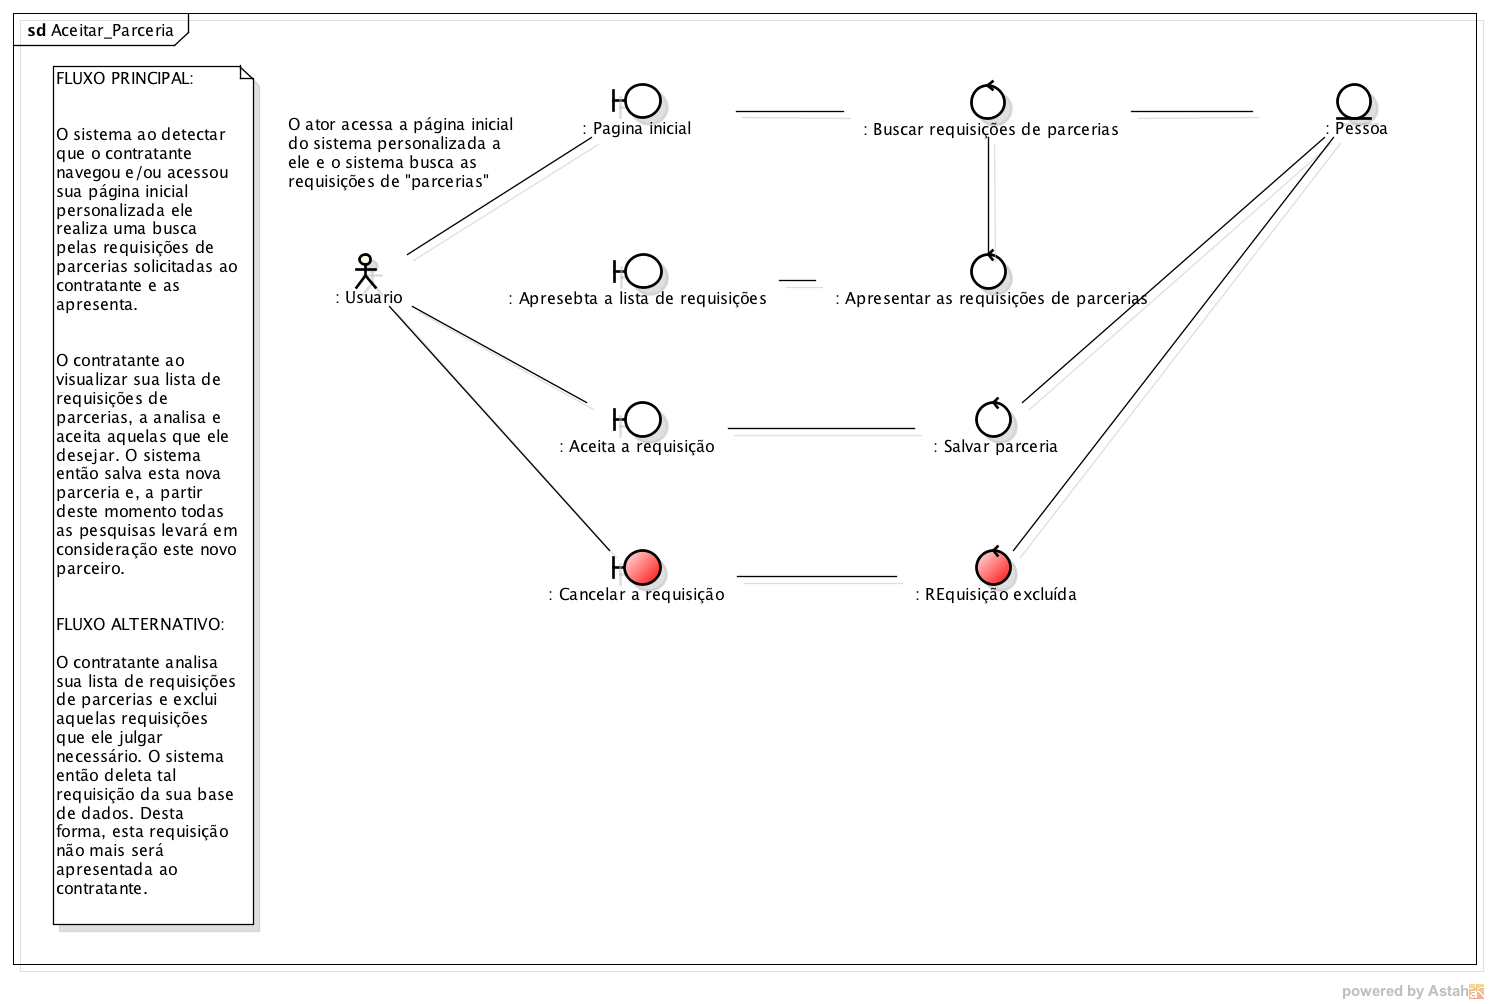
\includegraphics[scale=0.38]{./imagens/apendices/diagrama-robustez-aceitar-parceria.png}}
	\caption[Diagrama de robustez referente ao caso de uso ''Aceitar parceria''.]
	{Diagrama de robustez referente ao caso de uso ''Aceitar parceria''. \textbf{Fonte:} Elaborado pelos autores.}
	\label{fig:ap1:diagrama_robustez_aceitar_parceria}
\end{figure}

O próximo diagrama de robustez apresentado na Figura~\ref{fig:ap1:diagrama_robustez_localizar_parceiro} é referente ao caso de uso ''Localizar parceiro''.

\captionsetup[figure]{list=no}
\begin{figure}[h!]
	\centerline{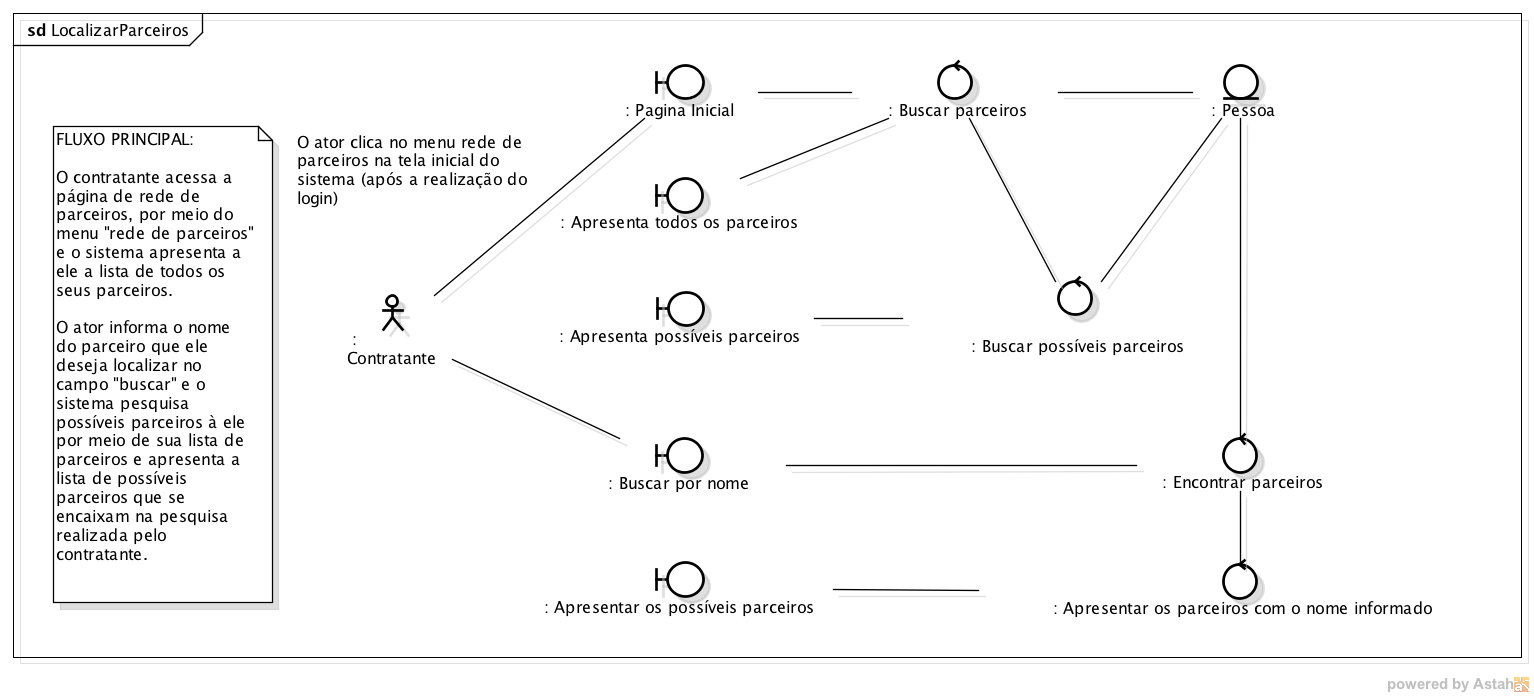
\includegraphics[scale=0.37]{./imagens/apendices/diagrama-robustez-localizar-parceiros.png}}
	\caption[Diagrama de robustez referente ao caso de uso ''Localizar parceiro''.]
	{Diagrama de robustez referente ao caso de uso ''Localizar parceiro''. \textbf{Fonte:} Elaborado pelos autores.}
	\label{fig:ap1:diagrama_robustez_localizar_parceiro}
\end{figure}

O próximo diagrama de robustez apresentado na Figura~\ref{fig:ap1:diagrama_robustez_adicionar_parceiro} é referente ao caso de uso ''Adicionar parceiro''.

\newpage
\captionsetup[figure]{list=no}
\begin{figure}[h!]
	\centerline{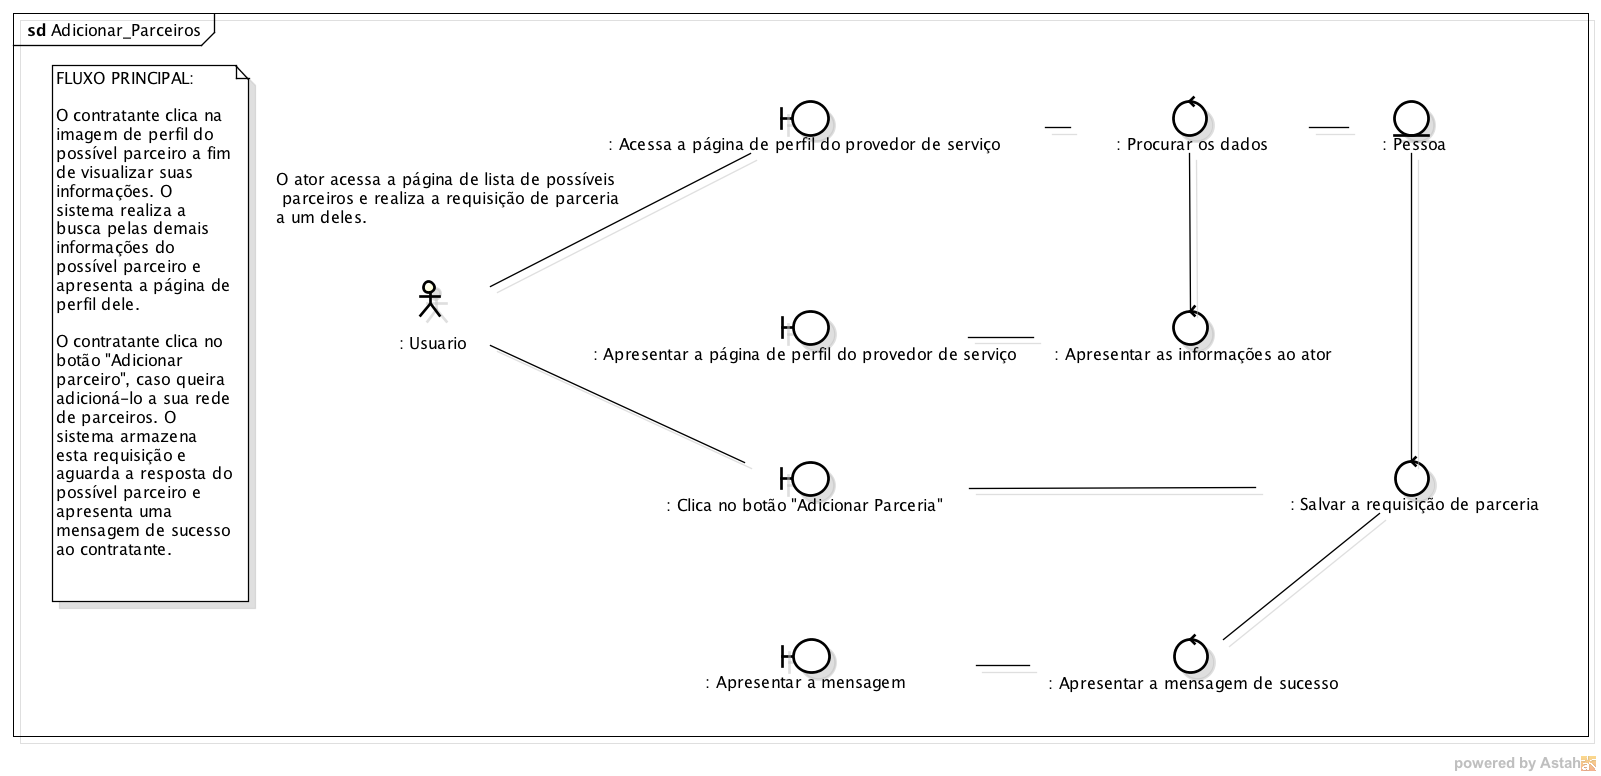
\includegraphics[scale=0.35]{./imagens/apendices/diagrama-robustez-adicionar-parceiro.png}}
	\caption[Diagrama de robustez referente ao caso de uso ''Adicionar parceiro''.]
	{Diagrama de robustez referente ao caso de uso ''Adicionar parceiro''. \textbf{Fonte:} Elaborado pelos autores.}
	\label{fig:ap1:diagrama_robustez_adicionar_parceiro}
\end{figure}

O próximo diagrama de robustez apresentado na Figura~\ref{fig:ap1:diagrama_robustez_localizar_mao_de_obra} é referente ao caso de uso ''Localizar mão de obra''.

\captionsetup[figure]{list=no}
\begin{figure}[h!]
	\centerline{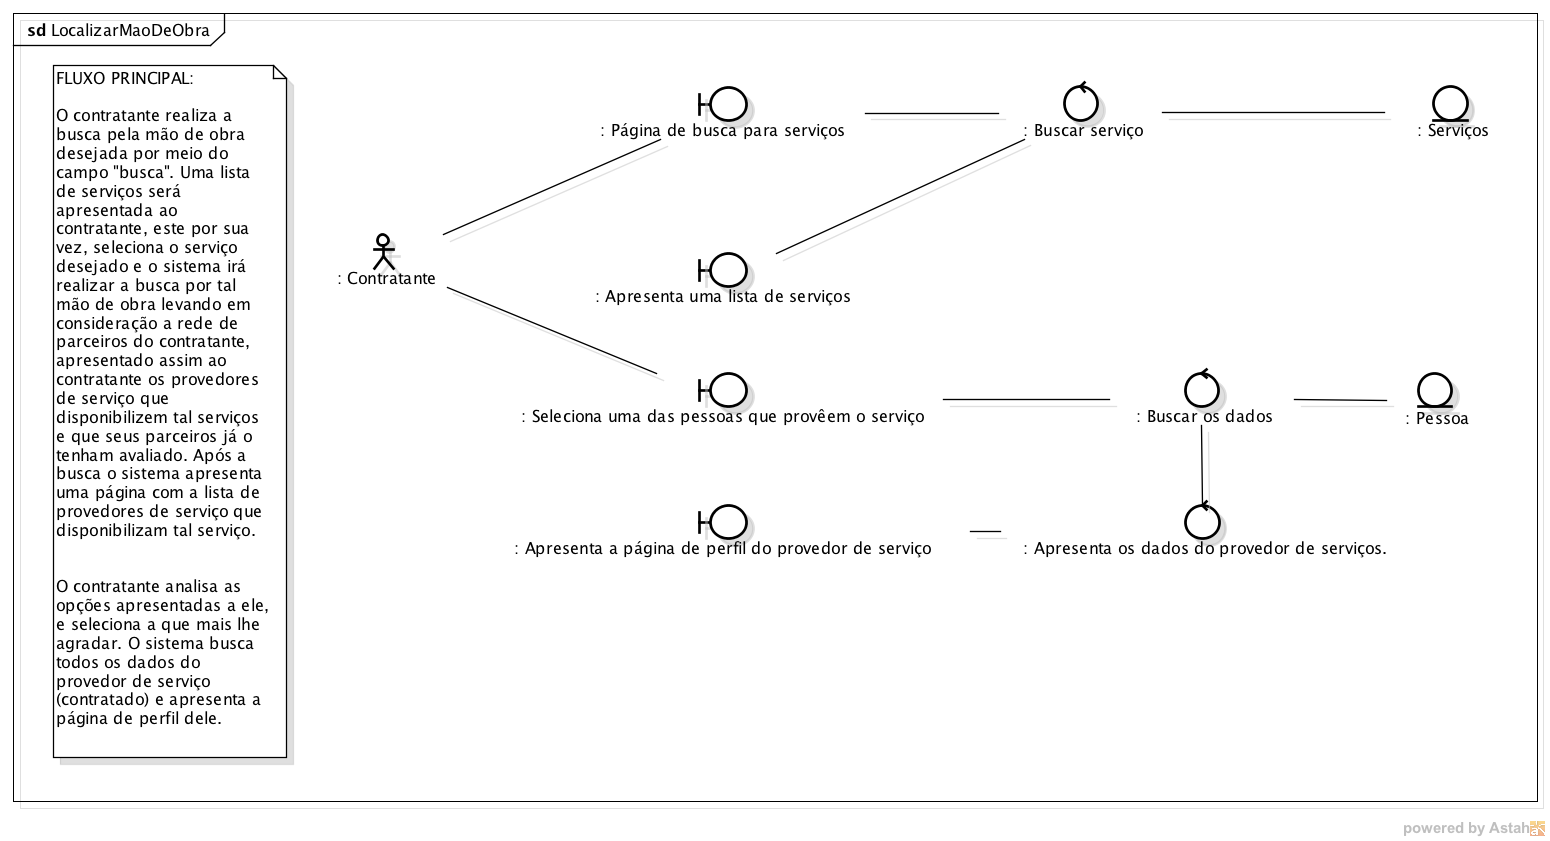
\includegraphics[scale=0.35]{./imagens/apendices/diagrama-robustez-localizar-mao-de-obra.png}}
	\caption[Diagrama de robustez referente ao caso de uso ''Localizar mão de obra''.]
	{Diagrama de robustez referente ao caso de uso ''Localizar mão de obra''. \textbf{Fonte:} Elaborado pelos autores.}
	\label{fig:ap1:diagrama_robustez_localizar_mao_de_obra}
\end{figure}

O próximo diagrama de robustez apresentado na Figura~\ref{fig:ap1:diagrama_robustez_avaliar_mao_de_obra} é referente ao caso de uso ''Avaliar mão de obra''.

\newpage
\captionsetup[figure]{list=no}
\begin{figure}[h!]
	\centerline{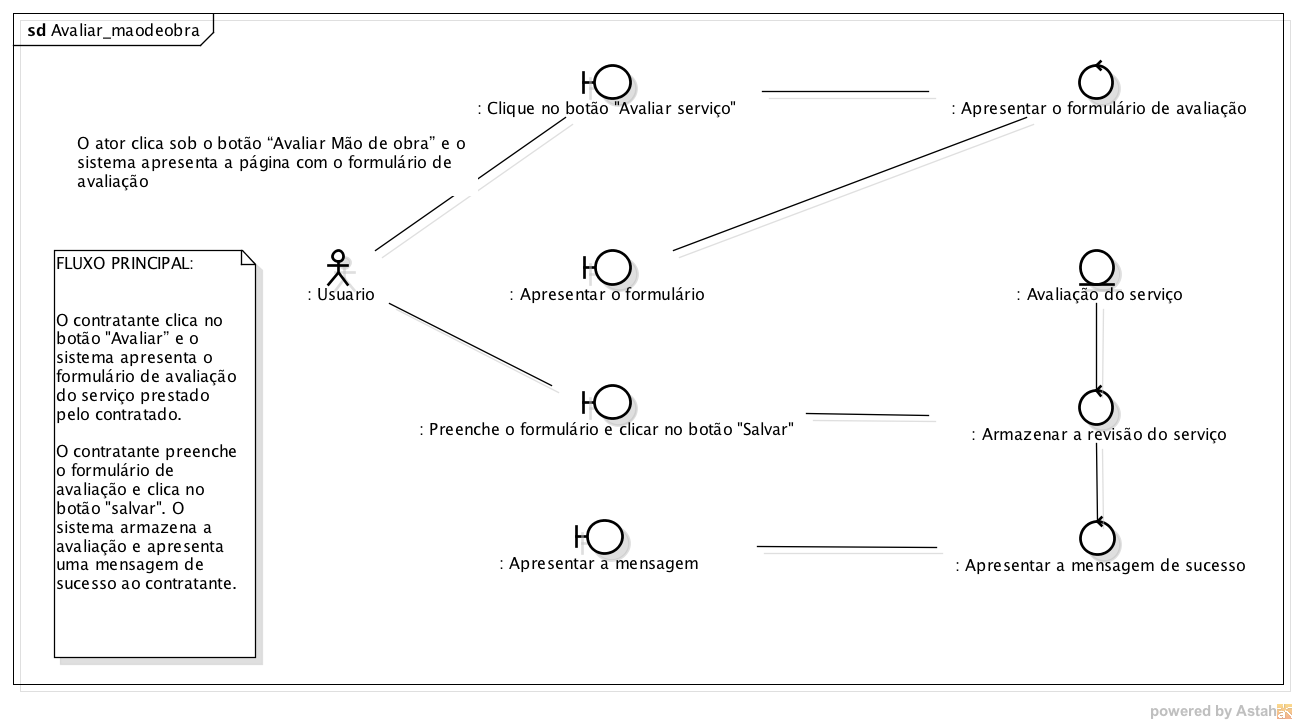
\includegraphics[scale=0.43]{./imagens/apendices/diagrama-robustez-avaliar-mao-de-obra.png}}
	\caption[Diagrama de robustez referente ao caso de uso ''Avaliar mão de obra''.]
	{Diagrama de robustez referente ao caso de uso ''Avaliar mão de obra''. \textbf{Fonte:} Elaborado pelos autores.}
	\label{fig:ap1:diagrama_robustez_avaliar_mao_de_obra}
\end{figure}

O próximo diagrama de robustez apresentado na Figura~\ref{fig:ap1:diagrama_robustez_gerenciar_servicos} é referente ao caso de uso ''Gerenciar serviços''.

\captionsetup[figure]{list=no}
\begin{figure}[h!]
	\centerline{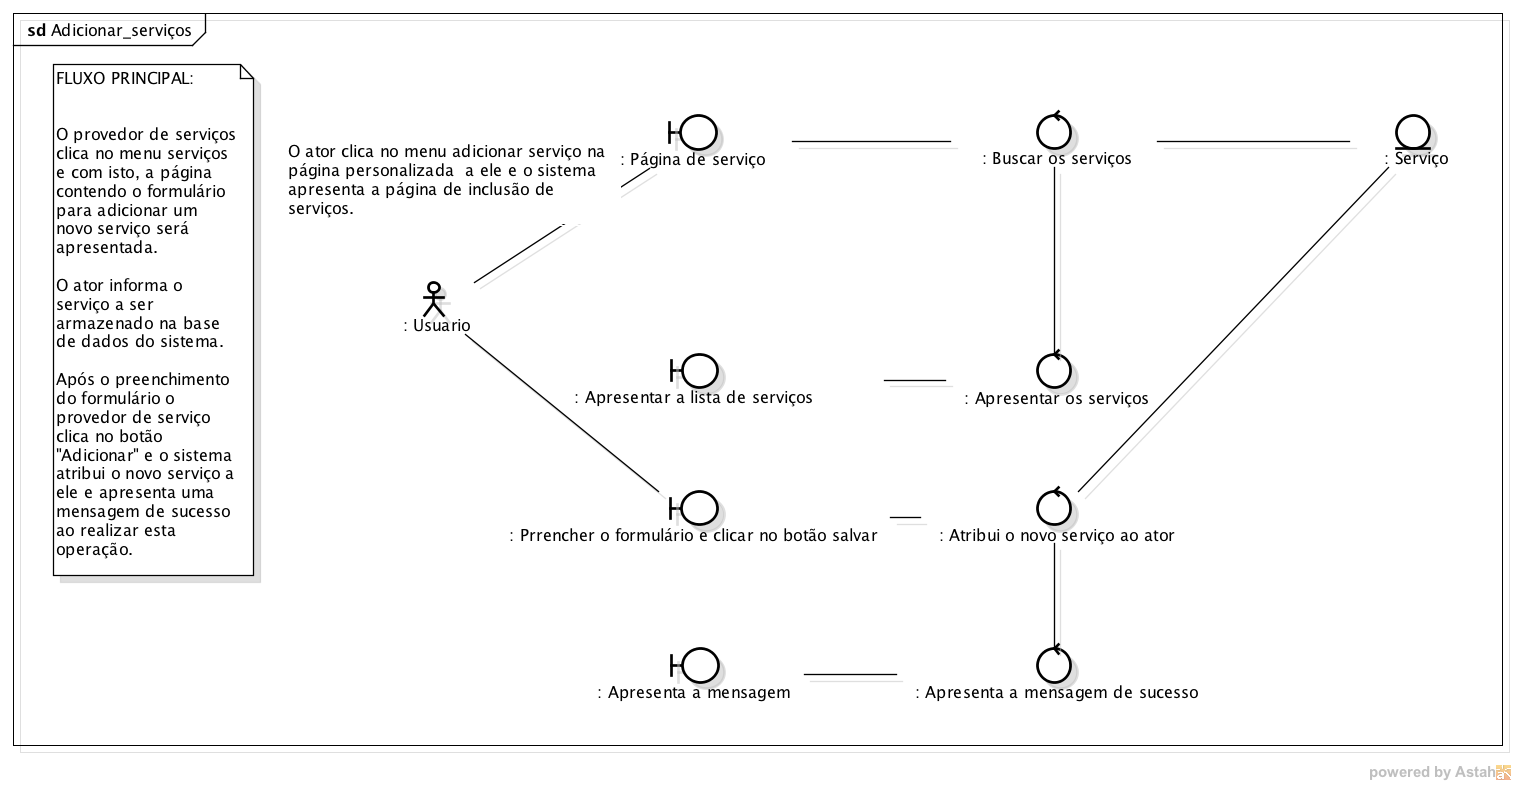
\includegraphics[scale=0.38]{./imagens/apendices/diagrama-robustez-adicionar-servicos.png}}
	\caption[Diagrama de robustez referente ao caso de uso ''Gerenciar serviços''.]
	{Diagrama de robustez referente ao caso de uso ''Gerenciar serviços''. \textbf{Fonte:} Elaborado pelos autores.}
	\label{fig:ap1:diagrama_robustez_gerenciar_servicos}
\end{figure}

O último diagrama de robustez apresentado na Figura~\ref{fig:ap1:diagrama_robustez_criar_conta} é referente ao caso de uso ''Criar conta''.

\newpage
\captionsetup[figure]{list=no}
\begin{figure}[h!]
	\centerline{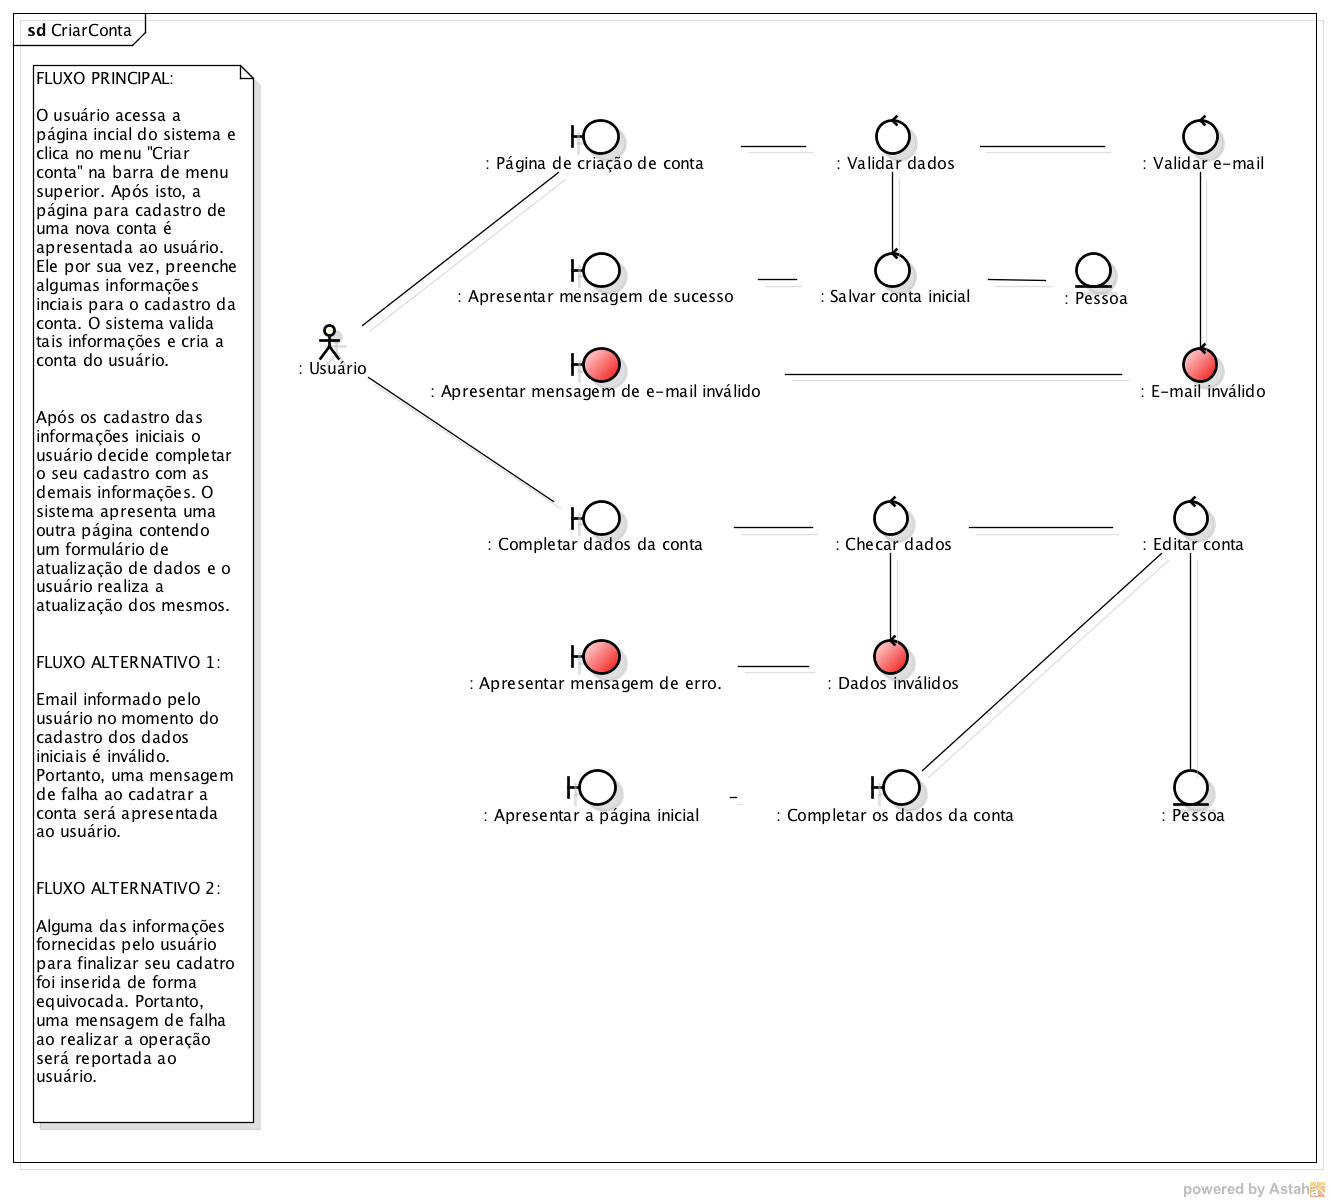
\includegraphics[scale=0.4]{./imagens/apendices/diagrama-robustez-criar-conta.png}}
	\caption[Diagrama de robustez referente ao caso de uso ''Criar conta''.]
	{Diagrama de robustez referente ao caso de uso ''Criar conta''. \textbf{Fonte:} Elaborado pelos autores.}
	\label{fig:ap1:diagrama_robustez_criar_conta}
\end{figure}

Após a criação dos diagramas de robustez, o diagrama de modelo de domínio foi atualizado, adicionando os atributos identificados pelos diagramas de caso de robustez, passando-se a trabalhar nos diagramas de sequência, que seão apresentados a seguir.

\section*{Diagramas de Sequência}

Os diagramas de sequência foram criados baseado-se no diagramas apresentados anteriormente. Seguindo a mesma ordem anteriormente definida, o primeiro diagrama de sequência apresentado na Figura~\ref{fig:ap1:diagrama_sequencia_aceitar_parceria} é referente ao caso de uso ''Aceitar parceria''.

\newpage
\captionsetup[figure]{list=no}
\begin{figure}[h!]
	\centerline{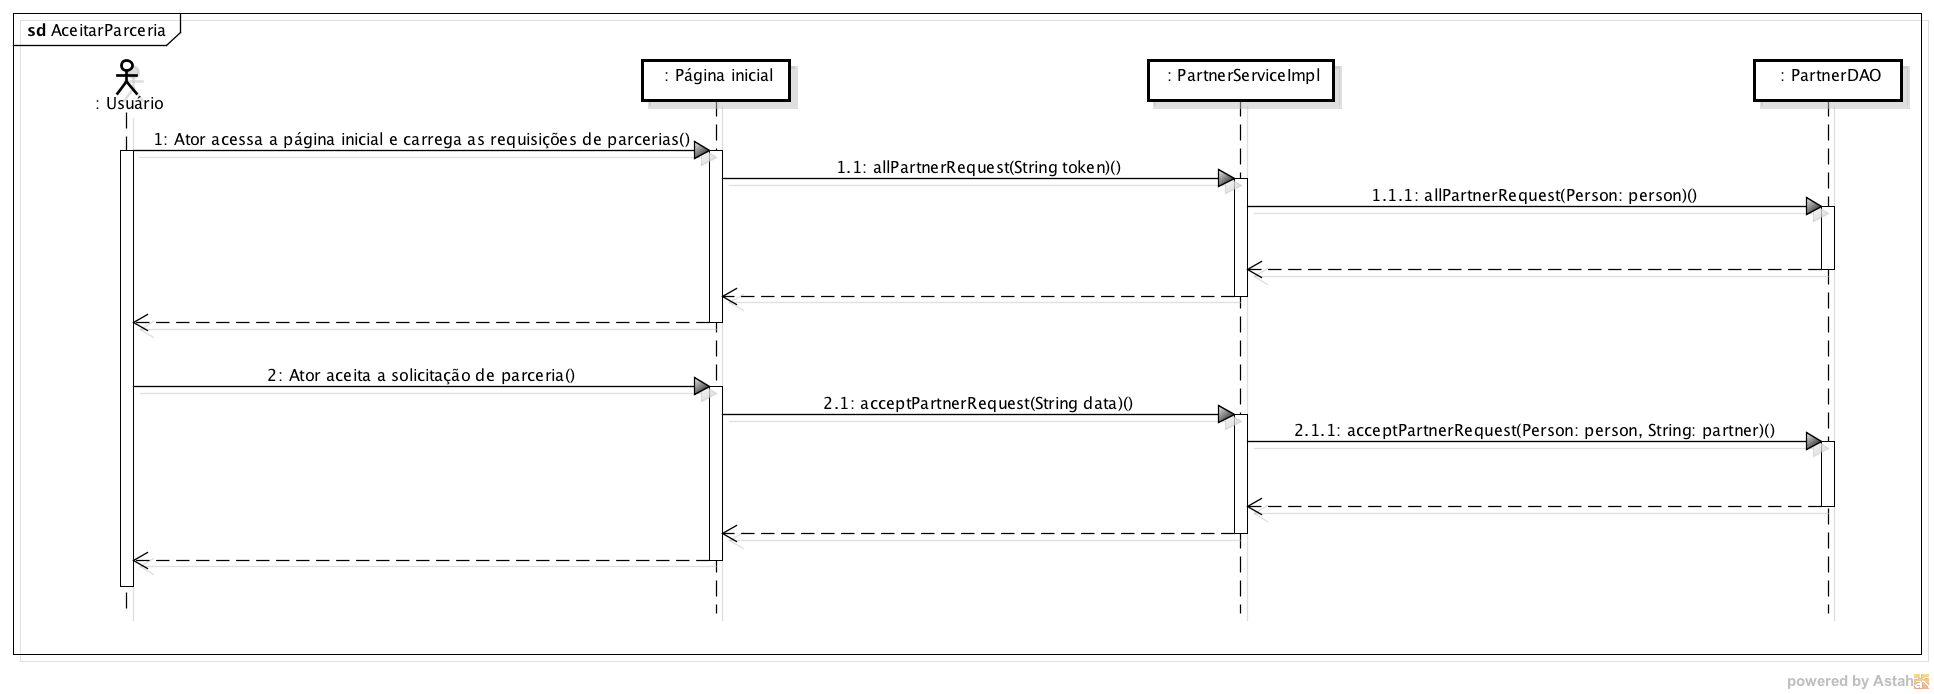
\includegraphics[angle=90,scale=0.42]{./imagens/apendices/diagrama-sequencia-aceitar-parceria.png}}
	\caption[Diagrama de sequência referente ao caso de uso ''Aceitar parceria''.]
	{Diagrama de sequência referente ao caso de uso ''Aceitar parceria''. \textbf{Fonte:} Elaborado pelos autores.}
	\label{fig:ap1:diagrama_sequencia_aceitar_parceria}
\end{figure}

O próximo diagrama de sequência apresentado na Figura~\ref{fig:ap1:diagrama_sequencia_localizar_parceiro} é referente ao caso de uso ''Localizar parceiro''.

\newpage
\captionsetup[figure]{list=no}
\begin{figure}[h!]
	\centerline{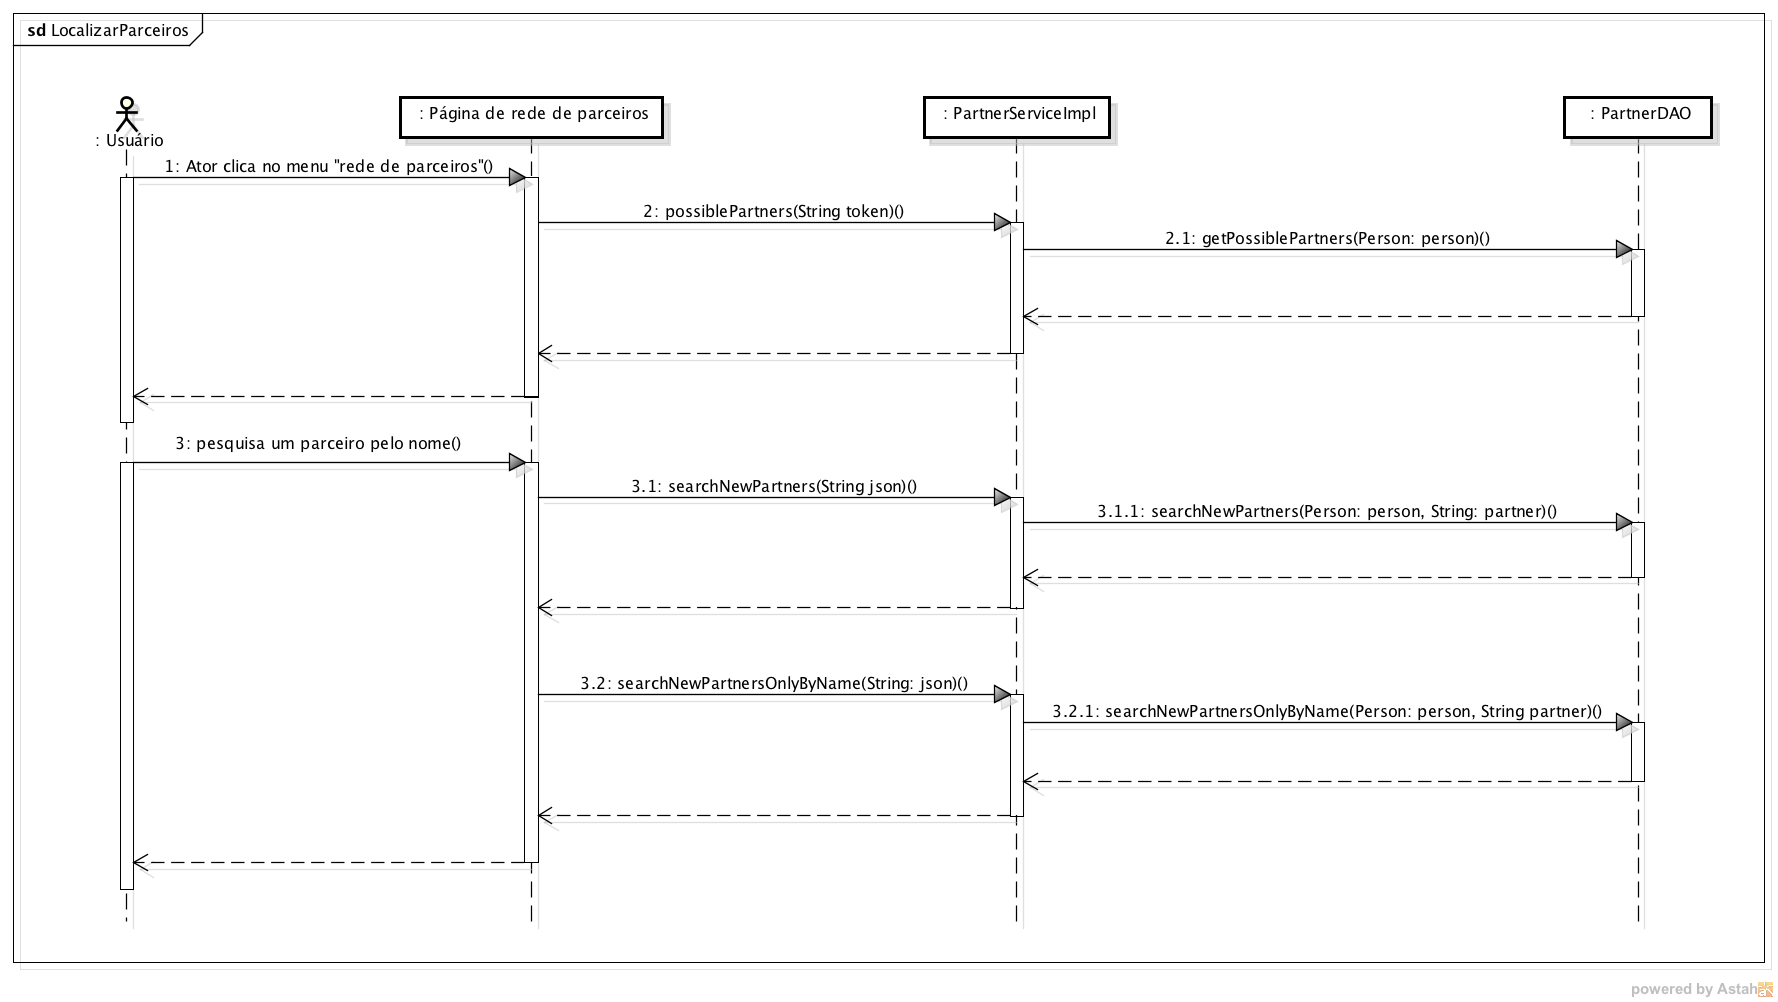
\includegraphics[angle=90,scale=0.42]{./imagens/apendices/diagrama-sequencia-localizar-parceiros.png}}
	\caption[Diagrama de sequência referente ao caso de uso ''Localizar parceiro''.]
	{Diagrama de sequência referente ao caso de uso ''Localizar parceiro''. \textbf{Fonte:} Elaborado pelos autores.}
	\label{fig:ap1:diagrama_sequencia_localizar_parceiro}
\end{figure}

O próximo diagrama de sequência apresentado na Figura~\ref{fig:ap1:diagrama_sequencia_adicionar_parceiro} é referente ao caso de uso ''Adicionar parceiro''.

\begin{landscape}
\newpage
\captionsetup[figure]{list=no}
\begin{figure}[h!]
	\centerline{\includegraphics[scale=0.3]{./imagens/apendices/diagrama-sequencia-adicionar-parceiros.png}}
	\caption[Diagrama de sequência referente ao caso de uso ''Adicionar parceiro''.]
	{Diagrama de sequência referente ao caso de uso ''Adicionar parceiro''. \textbf{Fonte:} Elaborado pelos autores.}
	\label{fig:ap1:diagrama_sequencia_adicionar_parceiro}
\end{figure}

O próximo diagrama de sequência apresentado na Figura~\ref{fig:ap1:diagrama_sequencia_localizar_mao_de_obra} é referente ao caso de uso ''Localizar mão de obra''.

\newpage
\captionsetup[figure]{list=no}
\begin{figure}[h!]
	\centerline{\includegraphics[scale=0.4]{./imagens/apendices/diagrama-sequencia-localizar-mao-de-obra.png}}
	\caption[Diagrama de sequência referente ao caso de uso ''Localizar mão de obra''.]
	{Diagrama de sequência referente ao caso de uso ''Localizar mão de obra''. \textbf{Fonte:} Elaborado pelos autores.}
	\label{fig:ap1:diagrama_sequencia_localizar_mao_de_obra}
\end{figure}

O próximo diagrama de sequência apresentado na Figura~\ref{fig:ap1:diagrama_sequencia_avaliar_mao_de_obra} é referente ao caso de uso ''Avaliar mão de obra''.

\newpage
\captionsetup[figure]{list=no}
\begin{figure}[h!]
	\centerline{\includegraphics[scale=0.2]{./imagens/apendices/diagrama-sequencia-avaliar-mao-de-obra.png}}
	\caption[Diagrama de sequência referente ao caso de uso ''Avaliar mão de obra''.]
	{Diagrama de sequência referente ao caso de uso ''Avaliar mão de obra''. \textbf{Fonte:} Elaborado pelos autores.}
	\label{fig:ap1:diagrama_sequencia_avaliar_mao_de_obra}
\end{figure}

O próximo diagrama de sequência apresentado na Figura~\ref{fig:ap1:diagrama_sequencia_gerenciar_servicos} é referente ao caso de uso ''Gerenciar serviços''.

\newpage
\captionsetup[figure]{list=no}
\begin{figure}[h!]
	\centerline{\includegraphics[scale=0.4]{./imagens/apendices/diagrama-sequencia-gerenciar-servicos.png}}
	\caption[Diagrama de sequência referente ao caso de uso ''Gerenciar serviços''.]
	{Diagrama de sequência referente ao caso de uso ''Gerenciar serviços''. \textbf{Fonte:} Elaborado pelos autores.}
	\label{fig:ap1:diagrama_sequencia_gerenciar_servicos}
\end{figure}

O último diagrama de sequência apresentado na Figura~\ref{fig:ap1:diagrama_sequencia_criar_conta} é referente ao caso de uso ''Criar conta''.

\captionsetup[figure]{list=no}
\begin{figure}[h!]
	\centerline{\includegraphics[scale=0.35]{./imagens/apendices/diagrama-sequencia-criar-conta.png}}
	\caption[Diagrama de sequência referente ao caso de uso ''Criar conta''.]
	{Diagrama de sequência referente ao caso de uso ''Criar conta''. \textbf{Fonte:} Elaborado pelos autores.}
	\label{fig:ap1:diagrama_sequencia_criar_conta}
\end{figure}
\end{landscape}

Após a criação dos diagramas de sequência, o diagrama de modelo de domínio foi atualizado, adicionando os atributos identificados pelos diagramas de sequência, gerando o diagrama de classes final.

\chapter*{Apêndice 2: API Rest}
\label{apendice:api_rest}

Nesse Apêndice será apresentado o contrato de serviços providos pelo \textit{Web Service} desenvolvido neste trabalho. Os serviços foram divididos em categorias, a fim de facilitar a compreensão dos contratos.

\section*{Estados e capitais}

\begin{lstlisting} [style=custom_XML,title={Contrato de serviço referente a estados e capitais. \textbf{Fonte:} Elaborado pelos autores.}, label=list:contrato_estados] 	
<application xmlns="http://wadl.dev.java.net/2009/02">
	<doc xml:lang="en" title="http://localhost:8080"/>
	<resources base="http://localhost:8080">
		<resource path="WebService/uf" id="uf">
			<doc xml:lang="en" title="uf"/>
			<method name="GET" id="uf">
				<doc xml:lang="en" title="uf"/>
				<request/>
				<response>
					<representation mediaType="application/json"/>
				</response>
			</method>
		</resource>
	<resources>
</application>
\end{lstlisting}


\section*{Cidades}

\begin{lstlisting} [style=custom_XML,title={Contrato de serviço referente a cidades. \textbf{Fonte:} Elaborado pelos autores.}, label=list:contrato_cidade] 	
<application xmlns="http://wadl.dev.java.net/2009/02">
	<doc xml:lang="en" title="http://localhost:8080"/>
	<resources base="http://localhost:8080">
		<resource path="WebService/city/cities/{state}" id="city">
			<doc xml:lang="en" title="city"/>
			<param name="state" type="xs:string" required="true" 
				default="" style="template" 
				xmlns:xs="http://www.w3.org/2001/XMLSchema"/>
			<method name="GET" id="city-cities">
				<doc xml:lang="en" title="city-cities"/>
				<request/>
				<response>
					<representation mediaType="application/json"/>
				</response>
			</method>
		</resource>
	<resources>
</application>
\end{lstlisting}


\section*{Sessão}

\begin{lstlisting} [style=custom_XML,title={Contrato de serviço referente a sessão do usuário autenticado. \textbf{Fonte:} Elaborado pelos autores.}, label=list:contrato_sessao] 	
<application xmlns="http://wadl.dev.java.net/2009/02">
	<doc xml:lang="en" title="http://localhost:8080"/>
	<resources base="http://localhost:8080">
		<resource path="WebService/session/userinfo/{token}" id="session">
			<doc xml:lang="en" title="session"/>
			<param name="token" type="xs:string" required="false" 
			default="" style="template" 
			xmlns:xs="http://www.w3.org/2001/XMLSchema"/>
			<method name="POST" id="session-login">
				<doc xml:lang="en" title="session-login"/>
				<request>
					<representation mediaType="application/json"/>
				</request>
				<response>
					<representation mediaType="application/json"/>
				</response>
			</method>
			<method name="GET" id="session-userinfo">
				<doc xml:lang="en" title="session-userinfo"/>
				<request/>
				<response>
					<representation mediaType="application/json"/>
				</response>
			</method>
		</resource>
	</resources>
</application>
\end{lstlisting}

\section*{Serviços}

\begin{lstlisting} [style=custom_XML,title={Contrato de serviço referente a serviços. \textbf{Fonte:} Elaborado pelos autores.}, label=list:contrato_servicos] 	
<application xmlns="http://wadl.dev.java.net/2009/02">
	<doc xml:lang="en" title="http://localhost:8080"/>
	<resources base="http://localhost:8080">
		<resource path="WebService/services/service/{name}" id="services">
			<doc xml:lang="en" title="services"/>
			<param name="name" type="xs:string" required="true"
			 default="" style="template" 
			 xmlns:xs="http://www.w3.org/2001/XMLSchema"/>
			<method name="GET" id="services-service">
				<doc xml:lang="en" title="services-service"/>
				<request/>
				<response>
					<representation mediaType="application/json"/>
				</response>
			</method>
		</resource>
	</resources>
</application>
\end{lstlisting}

\section*{Provedores de serviços}

\begin{lstlisting} [style=custom_XML,title={Contrato de serviço referente a provedores de serviços. \textbf{Fonte:} Elaborado pelos autores.}, label=list:contrato_provedores_servicos] 	
<application xmlns="http://wadl.dev.java.net/2009/02">
	<doc xml:lang="en" title="http://localhost:8080"/>
	<resource path="WebService/serviceprovider/removeservice" id="serviceprovider">
		<doc xml:lang="en" title="serviceprovider"/>
		<method name="GET" id="serviceprovider-byservice">
			<doc xml:lang="en" title="serviceprovider-byservice"/>
			<request/>
			<response>
				<representation mediaType="application/json"/>
			</response>
		</method>
		<method name="GET" id="serviceprovider-ratingInMyNetworkPartners">
			<doc xml:lang="en" title="serviceprovider-ratingInMyNetworkPartners"/>
			<request/>
			<response>
				<representation mediaType="application/json"/>
			</response>
		</method>
		<method name="GET" id="serviceprovider-ratingInMyCompany">
			<doc xml:lang="en" title="serviceprovider-ratingInMyCompany"/>
			<request/>
			<response>
				<representation mediaType="application/json"/>
			</response>
		</method>
		<method name="GET" id="serviceprovider-ratingInMyCity">
			<doc xml:lang="en" title="serviceprovider-ratingInMyCity"/>
			<request/>
			<response>
				<representation mediaType="application/json"/>
			</response>
		</method>
		<method name="GET" id="serviceprovider-data">
			<doc xml:lang="en" title="serviceprovider-data"/>
			<request/>
			<response>
				<representation mediaType="application/json"/>
			</response>
		</method>
		<method name="GET" id="serviceprovider-myservices">
			<doc xml:lang="en" title="serviceprovider-myservices"/>
			<request/>
			<response>
				<representation mediaType="application/json"/>
			</response>
		</method>
		<method name="POST" id="serviceprovider-addservice">
			<doc xml:lang="en" title="serviceprovider-addservice"/>
			<request>
				<representation mediaType="application/json"/>
			</request>
			<response>
				<representation mediaType="application/json"/>
			</response>
		</method>
		<method name="POST" id="serviceprovider-removeservice">
			<doc xml:lang="en" title="serviceprovider-removeservice"/>
			<request>
				<representation mediaType="application/json"/>
			</request>
			<response>
				<representation mediaType="application/json"/>
			</response>
		</method>
	</resource>
</application>
\end{lstlisting}

\section*{Avaliações de serviços}

\begin{lstlisting} [style=custom_XML,title={Contrato de serviço referente a avaliações de serviços. \textbf{Fonte:} Elaborado pelos autores.}, label=list:contrato_avaliacao_servicos] 	
<application xmlns="http://wadl.dev.java.net/2009/02">
	<doc xml:lang="en" title="http://localhost:8080"/>
	<resource path="WebService/rating/mylastestratings/{token}" id="rating">
		<doc xml:lang="en" title="rating"/>
		<param name="token" type="xs:string" required="true" 
		default="" style="template" 
		xmlns:xs="http://www.w3.org/2001/XMLSchema"/>
		<method name="POST" id="rating-save">
			<doc xml:lang="en" title="rating-save"/>
			<request>
				<representation mediaType="application/json"/>
			</request>
			<response>
				<representation mediaType="application/json"/>
			</response>
		</method>
		<method name="GET" id="rating-mylastestratings">
			<doc xml:lang="en" title="rating-mylastestratings"/>
			<request/>
			<response>
				<representation mediaType="application/json"/>
			</response>
		</method>
	</resource>	
</application>
\end{lstlisting}

\section*{Informações pessoais}

\begin{lstlisting} [style=custom_XML,title={Contrato de serviço referente a informações pessoais. \textbf{Fonte:} Elaborado pelos autores.}, label=list:contrato_informacoes_pessoais] 	
<application xmlns="http://wadl.dev.java.net/2009/02">
	<resource path="WebService/person/persondata/{partner}" id="person">
		<doc xml:lang="en" title="person"/>
		<param name="partner" type="xs:string" required="true"
		 default="" style="template" 
		 xmlns:xs="http://www.w3.org/2001/XMLSchema"/>
		<param name="token" type="xs:string" required="true"
		 default="" style="query" 
		 xmlns:xs="http://www.w3.org/2001/XMLSchema"/>
		<method name="POST" id="person-createaccount-personaldata">
			<doc xml:lang="en" title="person-createaccount-personaldata"/>
			<request>
				<representation mediaType="application/json"/>
			</request>
			<response>
				<representation mediaType="application/json"/>
			</response>
		</method>
		<method name="POST" id="person-createaccount-workdata">
			<doc xml:lang="en" title="person-createaccount-workdata"/>
			<request>
				<representation mediaType="application/json"/>
			</request>
			<response>
				<representation mediaType="application/json"/>
			</response>
		</method>
		<method name="GET" id="person-persondata">
			<doc xml:lang="en" title="person-persondata"/>
			<request/>
			<response>
				<representation mediaType="application/json"/>
			</response>
		</method>
	</resource>
</application>
\end{lstlisting}


\section*{Parceiros}

\begin{lstlisting} [style=custom_XML,title={Contrato de serviço referente a informações de paceiros. \textbf{Fonte:} Elaborado pelos autores.}, label=list:contrato_informacoes_de_parceiros] 	
<application xmlns="http://wadl.dev.java.net/2009/02">
	<resource path="WebService/partner/commonspartner/{partner}" id="partner">
		<doc xml:lang="en" title="partner"/>
		<param name="partner" type="xs:string" required="true" 
		default="" style="template" 
		xmlns:xs="http://www.w3.org/2001/XMLSchema"/>
		<param name="token" type="xs:string" required="true" 
		default="" style="query" 
		xmlns:xs="http://www.w3.org/2001/XMLSchema"/>
		<method name="GET" id="partner-possiblepartners">
			<doc xml:lang="en" title="partner-possiblepartners"/>
			<request/>
			<response>
				<representation mediaType="application/json"/>
			</response>
		</method>
		<method name="GET" id="partner-allpartners">
			<doc xml:lang="en" title="partner-allpartners"/>
			<request/>
			<response>
				<representation mediaType="application/json"/>
			</response>
		</method>
		<method name="POST" id="partner-add">
			<doc xml:lang="en" title="partner-add"/>
			<request>
				<representation mediaType="application/json"/>
			</request>
			<response>
				<representation mediaType="application/json"/>
			</response>
		</method>
		<method name="POST" id="partner-cancel">
			<doc xml:lang="en" title="partner-cancel"/>
			<request>
				<representation mediaType="application/json"/>
			</request>
			<response>
				<representation mediaType="application/json"/>
			</response>
		</method>
		<method name="GET" id="partner-allpartnerrequest">
			<doc xml:lang="en" title="partner-allpartnerrequest"/>
			<request/>
			<response>
				<representation mediaType="application/json"/>
			</response>
		</method>
		<method name="POST" id="partner-acceptpartnerrequest">
			<doc xml:lang="en" title="partner-acceptpartnerrequest"/>
			<request>
				<representation mediaType="application/json"/>
			</request>
			<response>
				<representation mediaType="application/json"/>
			</response>
		</method>
		<method name="POST" id="partner-rejectpartnerrequest">
			<doc xml:lang="en" title="partner-rejectpartnerrequest"/>
			<request>
				<representation mediaType="application/json"/>
			</request>
			<response>
				<representation mediaType="application/json"/>
			</response>
		</method>
		<method name="POST" id="partner-searchnewpartners">
			<doc xml:lang="en" title="partner-searchnewpartners"/>
			<request>
				<representation mediaType="application/json"/>
			</request>
			<response>
				<representation mediaType="application/json"/>
			</response>
		</method>
		<method name="POST" id="partner-searchnewpartnersonlybyname">
			<doc xml:lang="en" title="partner-searchnewpartnersonlybyname"/>
			<request>
				<representation mediaType="application/json"/>
			</request>
			<response>
				<representation mediaType="application/json"/>
			</response>
		</method>
		<method name="GET" id="partner-ismypartner">
			<doc xml:lang="en" title="partner-ismypartner"/>
			<request/>
			<response>
				<representation mediaType="application/json"/>
			</response>
		</method>
		<method name="GET" id="partner-commonspartner">
			<doc xml:lang="en" title="partner-commonspartner"/>
			<request/>
			<response>
				<representation mediaType="application/json"/>
			</response>
		</method>
	</resource>
</application>
\end{lstlisting}


\section*{Últimas atualizações}

\begin{lstlisting} [style=custom_XML,title={Contrato de serviço referente as últimas atualizações. \textbf{Fonte:} Elaborado pelos autores.}, label=list:contrato_ultimas_atualizacoes] 	
<application xmlns="http://wadl.dev.java.net/2009/02">
	<resource path="WebService/feed/lastestratings/{token}" id="feed">
		<doc xml:lang="en" title="feed"/>
		<param name="token" type="xs:string" required="false" 
		default="" style="template" 
		xmlns:xs="http://www.w3.org/2001/XMLSchema"/>
		<method name="GET" id="feed-lastestpartnership">
			<doc xml:lang="en" title="feed-lastestpartnership"/>
			<request/>
			<response>
				<representation mediaType="application/json"/>
			</response>
		</method>
		<method name="GET" id="feed-lastestratings">
			<doc xml:lang="en" title="feed-lastestratings"/>
			<request/>
			<response>
				<representation mediaType="application/json"/>
			</response>
		</method>
	</resource>
</application>
\end{lstlisting}

\section*{Gráficos}

\begin{lstlisting} [style=custom_XML,title={Contrato de serviço referente aos gráficos. \textbf{Fonte:} Elaborado pelos autores.}, label=list:contrato_graficos] 	
<application xmlns="http://wadl.dev.java.net/2009/02">
	<resource path="WebService/report/lastEvaluateInMyCity" id="report">
		<doc xml:lang="en" title="report"/>
		<param name="token" type="xs:string" required="true"
		 style="query" xmlns:xs="http://www.w3.org/2001/XMLSchema"/>
		<param name="service" type="xs:string" required="true"
		 style="query" xmlns:xs="http://www.w3.org/2001/XMLSchema"/>
		<param name="limit" type="xs:string" required="true"
		 style="query" xmlns:xs="http://www.w3.org/2001/XMLSchema"/>
		<method name="GET" id="report-lastEvaluateOfServiceProvider">
			<doc xml:lang="en" title="report-lastEvaluateOfServiceProvider"/>
			<request/>
			<response status="200">
				<representation mediaType="application/json"/>
			</response>
		</method>
		<method name="GET" id="report-lastEvaluateOfServiceInNetwork">
			<doc xml:lang="en" title="report-lastEvaluateOfServiceInNetwork"/>
			<request/>
			<response status="200">
				<representation mediaType="application/json"/>
			</response>
		</method>
		<method name="GET" id="report-lastEvaluate">
			<doc xml:lang="en" title="report-lastEvaluate"/>
			<request/>
			<response status="200">
				<representation mediaType="application/json"/>
			</response>
		</method>
		<method name="GET" id="report-lastEvaluateInMyCity">
			<doc xml:lang="en" title="report-lastEvaluateInMyCity"/>
			<request/>
			<response status="200">
				<representation mediaType="application/json"/>
			</response>
		</method>
	</resource>
</application>
\end{lstlisting}

Com este contrato definido foi possível dar continuidade no processo de desenvolvimento da aplicação.
\chapter*{Apêndice 3: Controlador de versão}
\label{ap3:github}

Neste Apêndice serão apresentados os passos necessários para a criação do repositório utilizado no sistema de controle de versão, junto com a instalação da ferramenta utilizada para trabalhar com este controlador de versão e sua configuração.

Para criar um repositório no GitHub (ferramenta de controle de versão) utilizado neste trabalho, deve-se acessar a  \textit{url} \texttt{http://github.com}, por meio de um navegador de internet e clicar no botão \textit{"Sign In"}, caso possua conta, caso contrário clique no botão \textit{"Sign up"} e crie sua conta. A Figura~\ref{fig:ap3:pagina_inicial_github} apresenta a página inicial do GitHub.

\captionsetup[figure]{list=no}
\begin{figure}[h!]
	\centerline{\includegraphics[scale=0.5]{./imagens/apendices/pagina-inicial-github.png}}
	\caption[Página inicial do GitHub.]
	{Página inicial do GitHub. \textbf{Fonte:} Elaborado pelos autores.}
	\label{fig:ap3:pagina_inicial_github}
\end{figure}

Para prosseguir com o processo de criação do repositório (com a conta já criada), deve-se clicar no botão \textit{"Sign In"} e realizar o \textit{login}. Após a conclusão desses passos a página inicial, contendo a lista de repositórios do usuário será apresentada conforme a Figura~\ref{fig:ap3:pagina_home_github} apresenta.

\newpage
\captionsetup[figure]{list=no}
\begin{figure}[h!]
	\centerline{\includegraphics[scale=0.5]{./imagens/apendices/pagina-home-github.png}}
	\caption[Página com a lista de repositórios do usuário no GitHub.]
	{Página com a lista de repositórios do usuário no GitHub. \textbf{Fonte:} Elaborado pelos autores.}
	\label{fig:ap3:pagina_home_github}
\end{figure}


Na página inicial deve-se clicar no botão \textit{"+ New Repository"} para que a página de criação do novo repositório seja apresentada conforme a Figura~\ref{fig:ap3:pagina_criacao_repository_github} apresenta.
\newpage
\captionsetup[figure]{list=no}
\begin{figure}[h!]
	\centerline{\includegraphics[scale=0.5]{./imagens/apendices/pagina-criacao-repositorio-github.png}}
	\caption[Página de criação de repositório no GitHub.]
	{Página de criação de repositório no GitHub. \textbf{Fonte:} Elaborado pelos autores.}
	\label{fig:ap3:pagina_criacao_repository_github}
\end{figure}

Nessa página deve-se informar os dados referentes ao repositório e, após preencher o formulário clique no botão \textit{"Create repository"}, a fim de concluir o processo de criação do repositório no GitHub.

Após criado o repositório, foi necessário adicionar os autores deste trabalho como colaboradores para que ambos pudessem modificar arquivos. Para fazer esta configuração é necessário clicar no menu \textit{"Settings"} da página inicial do repositório conforme apresenta a Figura~\ref{fig:ap3:pagina_inicial_repositororio_github}.

\newpage
\captionsetup[figure]{list=no}
\begin{figure}[h!]
	\centerline{\includegraphics[scale=0.5]{./imagens/apendices/pagina-inicial-repositorio-github.png}}
	\caption[Página do repositório no GitHub.]
	{Página do repositório no GitHub. \textbf{Fonte:} Elaborado pelos autores.}
	\label{fig:ap3:pagina_inicial_repositororio_github}
\end{figure}

Após clicar no menu \textit{"Settings"} é necessário navegar até a opção \textit{"Collaborators"} e informar o email ou o nome de usuário do colaborador conforme apresenta a Figura~\ref{fig:ap3:pagina_adicionar_colaborador_repositorio_github}.

\captionsetup[figure]{list=no}
\begin{figure}[h!]
	\centerline{\includegraphics[scale=0.5]{./imagens/apendices/pagina-adicionar-colaborador-ao-repositorio.png}}
	\caption[Página para adicionar um contribuidor ao repositório no GitHub.]
	{Página para adicionar um contribuidor ao repositório no GitHub. \textbf{Fonte:} Elaborado pelos autores.}
	\label{fig:ap3:pagina_adicionar_colaborador_repositorio_github}
\end{figure}

Após informar o dado do usuário e clicar no botão \textit{"Add collaborator"} o repositório estará pronto para ser utilizado. Para facilitar o manuseio de arquivos e suas respectivas versões, neste controlador de versão foi utlizada a ferramenta gráfica disponibilizada pelo GitHub a fim de facilitar a utilização deste sistema de controle de versão. Para realizar o download desta ferramenta, acesse a \textit{url} \texttt{https://desktop.github.com} por meio de um navegador de internet e clique no botão de download como apresenta a Figura~\ref{fig:ap3:pagina_download_github_para_windows}.

\captionsetup[figure]{list=no}
\begin{figure}[h!]
	\centerline{\includegraphics[scale=0.4]{./imagens/apendices/pagina-download-github.png}}
	\caption[Página de \textit{download} da ferramenta para gerenciamento de repositórios do GitHub.]
	{Página de \textit{download} da ferramenta para gerenciamento de repositórios do GitHub. \textbf{Fonte:} Elaborado pelos autores.}
	\label{fig:ap3:pagina_download_github_para_windows}
\end{figure}

Após realizar o download, deve-se executar o arquivo obtido por meio do processo de \textit{download} anteriormente mencionado. Após executá-lo, o processo de instalação da ferramenta irá iniciar, como apresenta a Figura~\ref{fig:ap3:instalacao_github_para_windows}.

\captionsetup[figure]{list=no}
\begin{figure}[h!]
	\centerline{\includegraphics[scale=0.5]{./imagens/apendices/instalacao-github-step1.png}}
	\caption[Instalação da ferramenta para gerenciamento de repositórios do GitHub.]
	{Instalação da ferramenta para gerenciamento de repositórios do GitHub. \textbf{Fonte:} Elaborado pelos autores.}
	\label{fig:ap3:instalacao_github_para_windows}
\end{figure}

Após concluir a instalação da ferramenta execute-a para configurar o repositório local no computador de trabalho. Com a aplicação em execução clique no botão "+" e em seguida, no menu \textit{"Clone"}, após esses passos localize o repositório desejado e clique em \textit{"Clone Repository"} como apresenta a Figura~\ref{fig:ap3:clonar_repositorio_github}.

\newpage
\captionsetup[figure]{list=no}
\begin{figure}[h!]
	\centerline{\includegraphics[scale=0.4]{./imagens/apendices/clonar-repositorio-github.png}}
	\caption[Processo para clonar repositório do GitHub.]
	{Processo para clonar repositório do GitHub. \textbf{Fonte:} Elaborado pelos autores.}
	\label{fig:ap3:clonar_repositorio_github}
\end{figure}

Após a realização dos passos descritos neste apêndice o repositório no GitHub estará totalmente configurado.
\chapter*{Eclipse e Tomcat}
\label{apendice:eclipse_tomcat}

Neste Apêndice serão apresentados os passos necessários para a instalação e configuração do Tomcat e do Eclipse (IDE de desenvolvimento utilizado neste trabalho).

\section*{Eclipse}

Para utilizar a IDE de desenvolvimento Eclipse, é necessário fazer o download dele por meio da \textit{url} https://eclipse.org/downloads/. Ao acessar esta \textit{url} a página de \textit{download} será apresentada ao usuário conforme a Figura~\ref{fig:ap2:pagina_download_eclipse}.

\captionsetup[figure]{list=no}
\begin{figure}[h!]
	\centerline{\includegraphics[scale=0.4]{./imagens/apendices/pagina-download-eclipse.png}}
	\caption[Página de \textit{download} do Eclipse.]
	{Página de \textit{download} do Eclipse. \textbf{Fonte:} Elaborado pelos autores.}
	\label{fig:ap2:pagina_download_eclipse}
\end{figure}

Nesta página o usuário deve selecionar qual a versão do sistema operacional ele utiliza para realizar o \textit{download} da versão correta.

Após realizado o download, o usuário deve descompactar o arquivo obtido e armazená-lo na pasta que desejar. Para iniciar o eclipse o usuário deve executar o arquivo eclipse.bat para sistemas operacionais Windows ou eclipse.sh para sistemas baseados em Unix como o Linux ou o OS X.

Após a executação deste arquivo o Eclipse, solicitará o diretório para criação do diretório de trabalho que ele irá utilizar, nesse momento o usuário deve informar um diretório válido. A Figura~\ref{fig:ap2:eclipse_selecionar_workspace} apresenta esta configuração.

\captionsetup[figure]{list=no}
\begin{figure}[h!]
	\centerline{\includegraphics[scale=0.5]{./imagens/apendices/eclipse-selecionar-workspace.png}}
	\caption[Tela de definição de diretório de trabalho do Eclipse.]
	{Tela de definição de diretório de trabalho do Eclipse. \textbf{Fonte:} Elaborado pelos autores.}
	\label{fig:ap2:eclipse_selecionar_workspace}
\end{figure}

Após realizar os procedimentos descritos nesta seção, a tela inicial do eclipse será apresentada ao usuário, que, nesse instante estará apto a utilizá-lo e realizar as devidas configurações.

\section*{Tomcat}

Para utilizar o Tomcat foi necessario fazer o \textit{download} dele por meio da \textit{url} https://tomcat.apache.org, após acessá-la, selecione a versão que deseja e clique sob ela. A Figura~\ref{fig:ap2:pagina_inicial_apache_tomcat}.

\newpage
\captionsetup[figure]{list=no}
\begin{figure}[h!]
	\centerline{\includegraphics[scale=0.35]{./imagens/apendices/pagina-inicial-apache-tomcat.png}}
	\caption[Página inicial do Tomcat.]
	{Página inicial do Tomcat. \textbf{Fonte:} Elaborado pelos autores.}
	\label{fig:ap2:pagina_inicial_apache_tomcat}
\end{figure}

Após a seleção da versão do Tomcat a página específica da versão selecionada será apresentada ao usuário conforme a Figura~\ref{fig:ap2:pagina_download_apache_tomcat}. Clique na opção desejada para realizar o \textit{download}. Neste trabalho foi utilizada a versão compactada do \textit{Core}.

\captionsetup[figure]{list=no}
\begin{figure}[h!]
	\centerline{\includegraphics[scale=0.4]{./imagens/apendices/pagina-download-tomcat-7.png}}
	\caption[Página para \textit{download} do Tomcat.]
	{Página para \textit{download} do Tomcat. \textbf{Fonte:} Elaborado pelos autores.}
	\label{fig:ap2:pagina_download_apache_tomcat}
\end{figure}

Após o processo de \textit{dowload} concluído, deve-se descompactar o arquivo obtido em um diretório.

\subsection*{Configuração do Tomcat}

Para utilizar o Tomcat em conjunto com o Eclipse, foi necessário realizar algumas configurações que serão apresentadas a seguir.

Com o Eclipse sendo executado, abra a perspectiva \textit{Server} como demonstra a Figura~\ref{fig:ap2:perspectiva_server_no_server_eclipse} e clique no \textit{link} apresentado.

\captionsetup[figure]{list=no}
\begin{figure}[h!]
	\centerline{\includegraphics[scale=0.5]{./imagens/apendices/perspectiva-server-sem-servidor.png}}
	\caption[Perspectiva \textit{Server} do Eclipse.]
	{Perspectiva \textit{Server} do Eclipse. \textbf{Fonte:} Elaborado pelos autores.}
	\label{fig:ap2:perspectiva_server_no_server_eclipse}
\end{figure}

Uma nova tela será apresentada solicitando ao usuário que selecione a versão do servidor que deseja adicionar como mostra a Figura~\ref{fig:ap2:selecioanr_versao_server_adicionar_eclipse}, após esta definição clique no botão \textit{"Next"}.

\captionsetup[figure]{list=no}
\begin{figure}[h!]
	\centerline{\includegraphics[scale=0.4]{./imagens/apendices/criar-configuracao-tomcat-no-eclipse.png}}
	\caption[Definir a versão do novo servidor no Eclipse.]
	{Definir a versão do novo servidor no Eclipse. \textbf{Fonte:} Elaborado pelos autores.}
	\label{fig:ap2:selecioanr_versao_server_adicionar_eclipse}
\end{figure}

Após selecionar a versão do Tomcat, deve-se informar na próxima tela, como apresenta a Figura~\ref{fig:ap2:definir_diretorio_tomcat_no_eclipse}, as informações a respeito do diretório cujo Tomcat foi extraído e, sob qual versão do Java ele será executado, com essas informações definidas clique no botão \textit{"Finish"}.

\newpage
\captionsetup[figure]{list=no}
\begin{figure}[h!]
	\centerline{\includegraphics[scale=0.4]{./imagens/apendices/definir-pasta-home-tomcat.png}}
	\caption[Definir as configurações do Tomcat no Eclipse.]
	{Definir as configurações do Tomcat no Eclipse. \textbf{Fonte:} Elaborado pelos autores.}
	\label{fig:ap2:definir_diretorio_tomcat_no_eclipse}
\end{figure}

Após realizado todos os procedimentos descritos neste Apêndice, a IDE Eclipse em conjunto com o Tomcat estarão prontos para serem utilizados.

\chapter*{Apêndice 5: Banco de dados Neo4j}
\label{apendice:neo4j}

Neste Apêndice serão apresentados os passos para a instalação do banco de dados Neo4j.

\par Para realizar o \textit{download} do instalador do banco de dados Neo4j, deve-se acessar a seguinte URL, por meio de um  navegador de internet: \texttt{http://neo4j.com/download} e selecionar a opção desejada. Neste trabalho como já descrito foi utilizada a versão \textit{Community}. A Figura~\ref{fig:ap3:download_neo4j} apresenta a página de \textit{download} do Neo4j.

\captionsetup[figure]{list=no}
\begin{figure}[h!]
	\centerline{\includegraphics[scale=0.4]{./imagens/apendices/download-neo4j.png}}
	\caption[Página de \textit{download} do Neo4j]
	{Página de \textit{download} do Neo4j. \textbf{Fonte:} http://neo4j.com/download}
	\label{fig:ap3:download_neo4j}
\end{figure}

\par Após concluído o \textit{download}, deve-se executar o arquivo. O processo de instalação se inicia e a primeira tela apresentada ao usuário é a tela contendo uma mensagem de boas vindas, conforme demonstra a Figura~\ref{fig:ap3:boas_vindas_neo4j}. Nesta tela, deve-se clicar no botão \textit{Next} para prosseguir com o processo de instalação.

\newpage
\captionsetup[figure]{list=no}
\begin{figure}[h!]
	\centerline{\includegraphics[scale=0.4]{./imagens/apendices/neo4j-install-step1.png}}
	\caption[Tela de boas vindas da instalação do Neo4j]
	{Tela de boas vindas da instalação do Neo4j. \textbf{Fonte:} Elaborado pelos autores.}
	\label{fig:ap3:boas_vindas_neo4j}
\end{figure}

\par A próxima tela apresentada ao usuário diz respeito ao contrato de uso do \textit{software}, como mostra a Figura~\ref{fig:ap3:contrato_neo4j}. Após lê-lo, deve-se aceitar os termos do contrato e clicar em \textit{Next}.

\captionsetup[figure]{list=no}
\begin{figure}[h!]
	\centerline{\includegraphics[scale=0.4]{./imagens/apendices/neo4j-install-step2.png}}
	\caption[Tela do contrato de uso do Neo4j]
	{Tela do contrato de uso do Neo4j. \textbf{Fonte:} Elaborado pelos autores.}
	\label{fig:ap3:contrato_neo4j}
\end{figure}

\par Na próxima tela, conforme a Figura~\ref{fig:ap3:definicao_diretorio_neo4j} demonstra, é definido o diretório de instalação do Neo4j. Por padrão este diretório é o mesmo das demais aplicações no \textit{Windows}, podendo ser alterado conforme a necessidade. Após definir o diretório de instalação deve-se clicar no botão \textit{Next}.

\captionsetup[figure]{list=no}
\begin{figure}[h!]
	\centerline{\includegraphics[scale=0.4]{./imagens/apendices/neo4j-install-step3.png}}
	\caption[Tela para definição do diretório de instalação do Neo4j]
	{Tela para definição do diretório de instalação do Neo4j. \textbf{Fonte:} Elaborado pelos autores.}
	\label{fig:ap3:definicao_diretorio_neo4j}
\end{figure}

\par Após as definições anteriores, uma tela é apresentada questionando o usuário a respeito da criação de atalhos na área de trabalho, como é demonstrado na Figura~\ref{fig:ap3:criacao_atalho_neo4j}. Posterior à definição dos atalhos do Neo4j, deve-se clicar no botão \textit{Next}.

\captionsetup[figure]{list=no}
\begin{figure}[h!]
	\centerline{\includegraphics[scale=0.4]{./imagens/apendices/neo4j-install-step4.png}}
	\caption[Tela para criação de atalhos do Neo4j]
	{Tela para criação de atalhos do Neo4j. \textbf{Fonte:} Elaborado pelos autores.}
	\label{fig:ap3:criacao_atalho_neo4j}
\end{figure}

\par Após realizar os procedimentos descritos para a instalação do Neo4j a tela final de instalação será apresentada, informando-o a respeito do resultado da instalação conforme demonstra a Figura~\ref{fig:ap3:tela_final_neo4j}. Clique no botão \textit{Finish} para finalizar o processo de instalação.
Após todos os passos realizados com sucesso, o Neo4j estará disponível.

\captionsetup[figure]{list=no}
\begin{figure}[h!]
	\centerline{\includegraphics[scale=0.4]{./imagens/apendices/neo4j-install-step5.png}}
	\caption[Tela final de instalação do Neo4j]
	{Tela final de instalação do Neo4j. \textbf{Fonte:} Elaborado pelos autores.}
	\label{fig:ap3:tela_final_neo4j}
	
\end{figure}

\par A Figura~\ref{fig:ap3:tela_inicial_neo4j} apresenta a tela inicial do Neo4j após sua instalação. Para iniciar a utilização desse banco de dados, clique no botão \textit{"Start"}.

\captionsetup[figure]{list=no}
\begin{figure}[h!]
	\centerline{\includegraphics[scale=0.60]{./imagens/apendices/neo4j.jpg}}
	\caption[Tela de inicialização do Neo4j ]
	{Tela de inicialização do Neo4j \textbf{Fonte:} Elaborado pelos autores.}
	\label{fig:ap3:tela_inicial_neo4j}
\end{figure}

\par Após realizar todos os procedimentos descritos neste apêndice o banco de dados Neo4j estará pronto para ser utilizado.

%\captionsetup[figure]{list=no}
%\begin{figure}[h!]
% \centerline{\includegraphics[scale=0.3]{./imagens/apendice_img1.png}}
% \caption[Outra imagem ainda.]
%           {Outra imagem ainda. \textbf{Fonte:} Elaborado pelos autores}
%  \label{fig:ap2:identificador}
%\end{figure}

%\section*{Segunda seção do apêndice 2}


%\par Continuando \ldots na figura Figura~\ref{fig:xml_exemplo} é mostrado um exemplo de XML.

%\begin{figure}[h!]
%\begin{lstlisting}[style=custom_XML]
%<project>
%...
% <dependencies>
%  ...
%  <dependency>
%   <groupId>org.neo4j</groupId>
%   <artifactId>neo4j</artifactId>
%   <version>1.9.4</version>
%  </dependency>
%  ...
% </dependencies>
% ...
%</project>
%\end{lstlisting}  
% \caption[Exemplo de código XML.]
%           {Exemplo de código XML. \textbf{Fonte:} Elaborado pelos autores}
%  \label{fig:xml_exemplo}
%\end{figure}


\chapter*{Apêndice 6: Questionário}
\label{apendice:questionario}

Nesse Apêndice será apresentado o questionário disponibilizado na internet e que foi utilizado para identificar a viabilidade desta pesquisa para a região de Pouso Alegre e sul de Minas Gerais.

Esse questionário teve como título ''Busca por mão de obra qualificada''. A fim de facilitar o tratamento e manipulação das respostas obtidas, foram utilizadas perguntas que seguirão o padrão de multipla escolhas. As perguntas utilizadas nessa pesquisa em conjunto respectivas opções são apresentadas a seguir:

\begin{enumerate}
	\item Qual das situações abaixo é a sua situação atual?
	\begin{enumerate}[label=(\alph*)]
		\item Moro com meus familiares;
		\item Moro em uma república com amigos;
		\item Moro sozinho.
	\end{enumerate}
	
	\item Como é a sua rotina de trabalho?
	\begin{enumerate}[label=(\alph*)]
		\item Fico o dia todo fora;
		\item Fico um período do dia fora;
		\item Trabalho em casa.
	\end{enumerate}
	
	\item Referente aos trabalhos domésticos e rotineiros, como você os realiza?
	\begin{enumerate}[label=(\alph*)]
		\item Eu mesmo faço os trabalhos no tempo vago;
		\item Contrato um profissional temporário para cuidar do trabalho;
		\item Raramente os realizo.
	\end{enumerate}

	\item Encontra dificuldade para encontrar mão de obra temporária? Tais como babá, encanador, pedreiro, etc.
	\begin{enumerate}[label=(\alph*)]
		\item Sim, encontro dificuldades;
		\item Não, encontro facilmente;
		\item Não utilizo.
	\end{enumerate}
	
	\item Quando você precisa destes tipos de serviços, qual das opções abaixo você considera ser o principal motivo da dificuldade de encontrá-los:
	\begin{enumerate}[label=(\alph*)]
		\item Este tipo de trabalho está escasso;
		\item Preciso de alguém de confiança;
		\item O custo está muito alto.
	\end{enumerate}
	
	\item Gostaria de um aplicativo para ajudar a encontrar este tipo de profissional?
	\begin{enumerate}[label=(\alph*)]
		\item Sim, seria muito útil;
		\item Não, não ajudaria;
		\item Talvez possa ser útil.
	\end{enumerate}	
\end{enumerate}


Com este questionário foi possível verificar a viabilidade deste trabalho no ambito social na região do sul de Minas Gerais, uma vez que foi obtido mais de cento e vinte respostas e cerca de 75\% demonstrou interesse nesse tipo de aplicação. 


\end{apendicesenv}
%%\anexoname{ANEXOS}
%\begin{anexosenv}
%\partanexos
%\chapter*{ANEXO I}

%\end{anexosenv}

\addcontentsline{toc}{chapter}{ANEXOS}

\chapter*{ANEXO I}



\printindex

\end{document}